\section{Размерная структура {\it Macoma balthica} в исследованных поселениях}
\label{app:sizestr_hist}

На всех графиках абсцисса --- длина раковины, мм; ордината --- численность особей, экз./м$^2$. Указано средняя численность особей определенного размера $\pm$ ошибка средней.

%Эстуарий Лувеньги
	\begin{figure}[hp]

	\begin{minipage}[b]{.3\linewidth}
	\begin{center}
	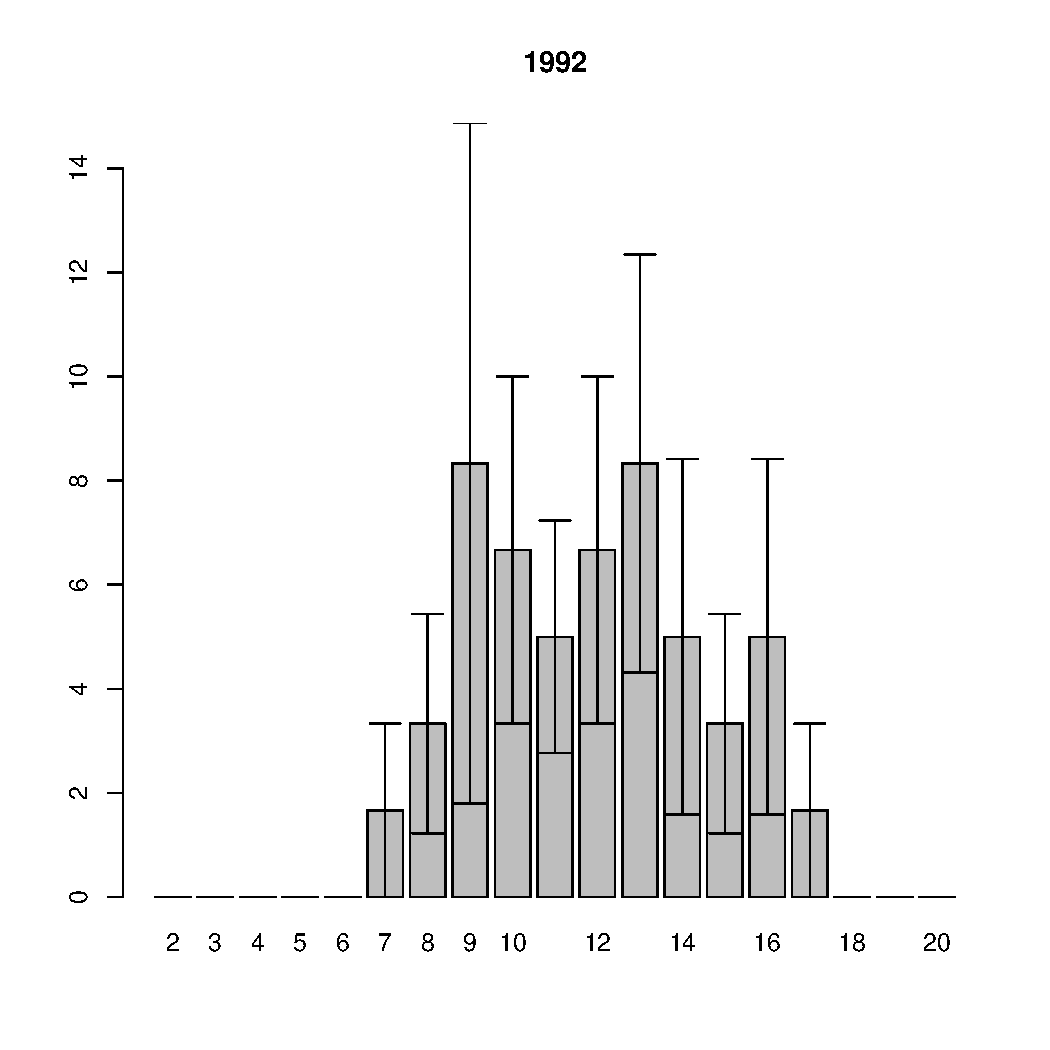
\includegraphics[width=60mm]{../White_Sea/Estuatiy_Luvenga/sizestr2_1992_.pdf}	
	\end{center}
	\end{minipage}
	%
	\hfil %Это пружинка отодвигающая рисунки друг от друга
	%
	\begin{minipage}[b]{.3\linewidth}
	\begin{center}
	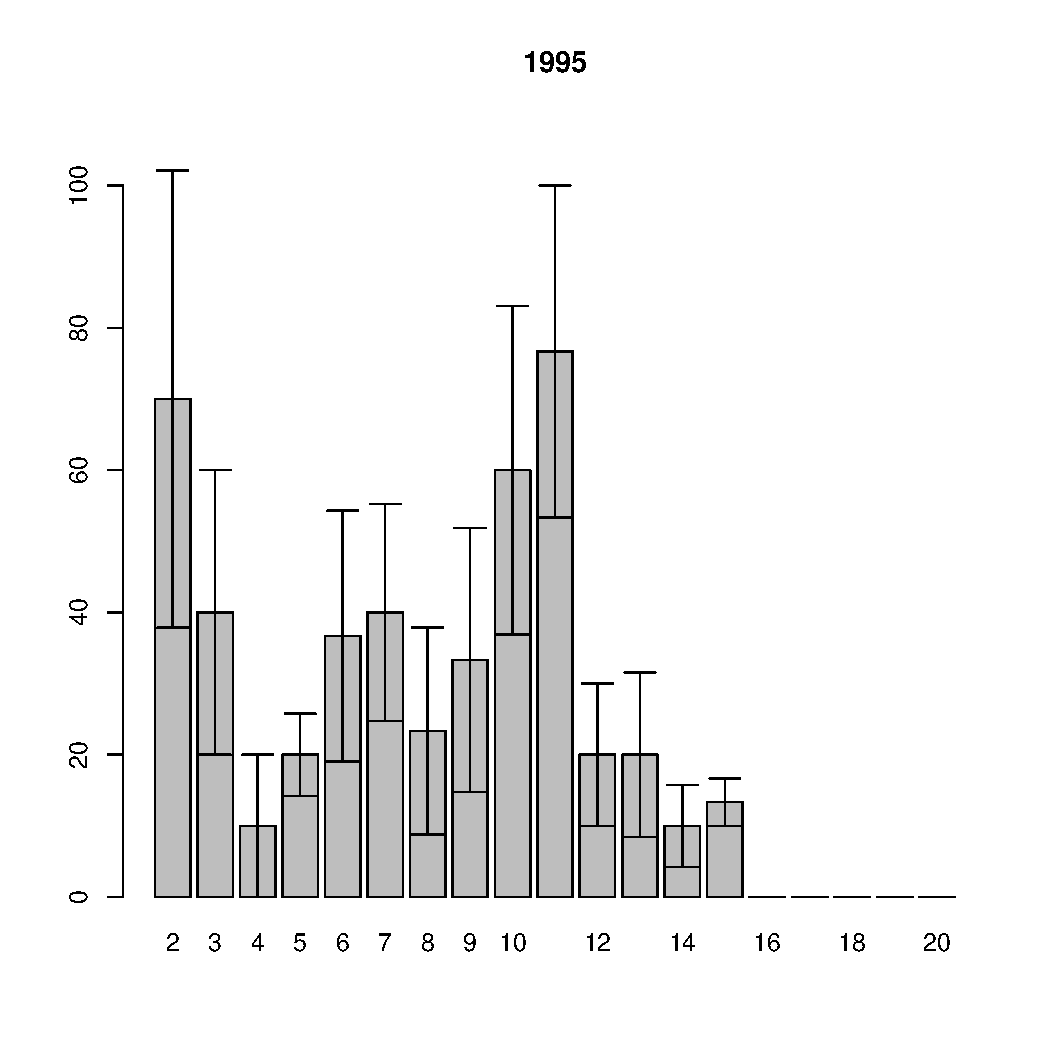
\includegraphics[width=60mm]{../White_Sea/Estuatiy_Luvenga/sizestr2_1995_.pdf}
	\end{center}
	\end{minipage}
	%
	\hfil %Это пружинка отодвигающая рисунки друг от друга
	%
	\begin{minipage}[b]{.3\linewidth}
	\begin{center}
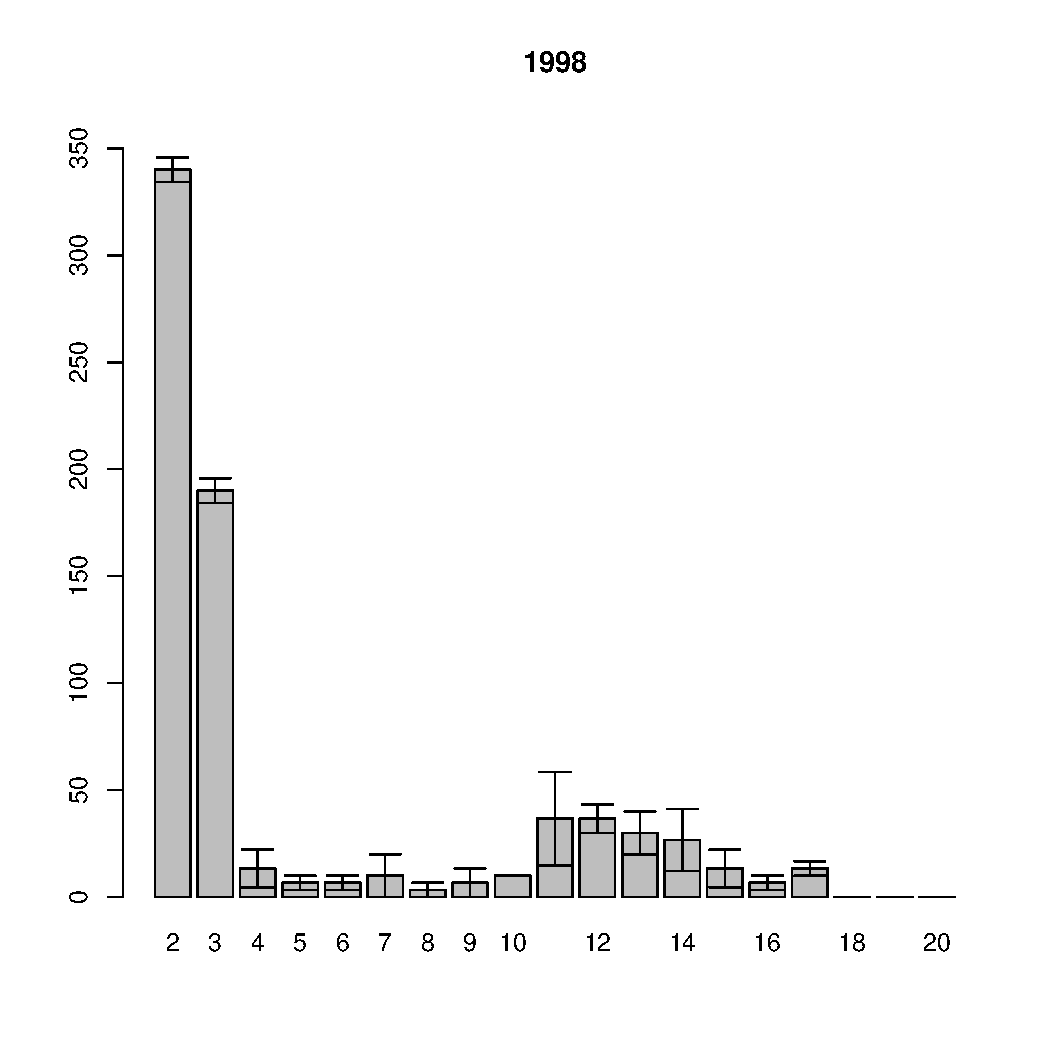
\includegraphics[width=60mm]{../White_Sea/Estuatiy_Luvenga/sizestr2_1998_.pdf}
	\end{center}
	\end{minipage}
	%
	\begin{minipage}[b]{.3\linewidth}
	\begin{center}
	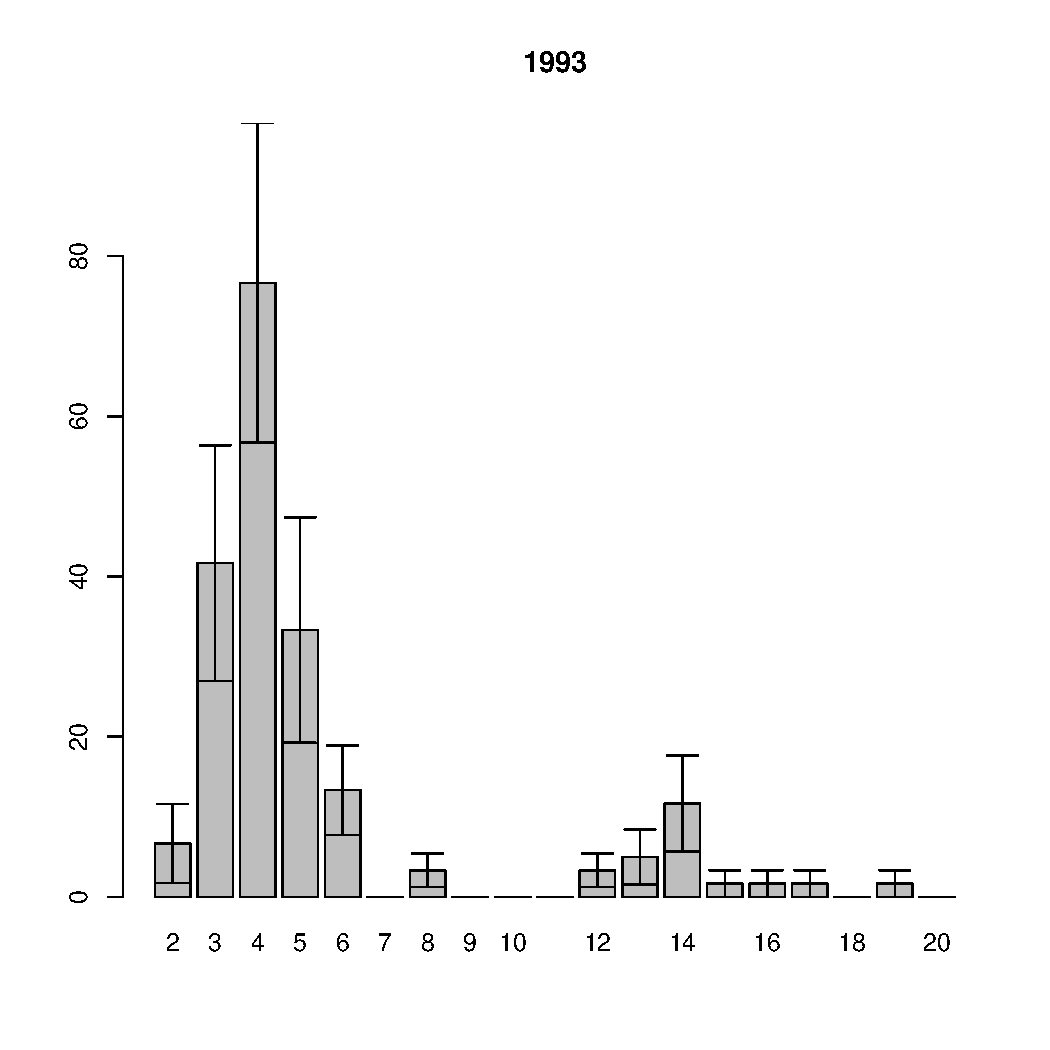
\includegraphics[width=60mm]{../White_Sea/Estuatiy_Luvenga/sizestr2_1993_.pdf}
	\end{center}
	\end{minipage}
	%
	\hfil %Это пружинка отодвигающая рисунки друг от друга
	%
	\begin{minipage}[b]{.3\linewidth}
	\begin{center}
	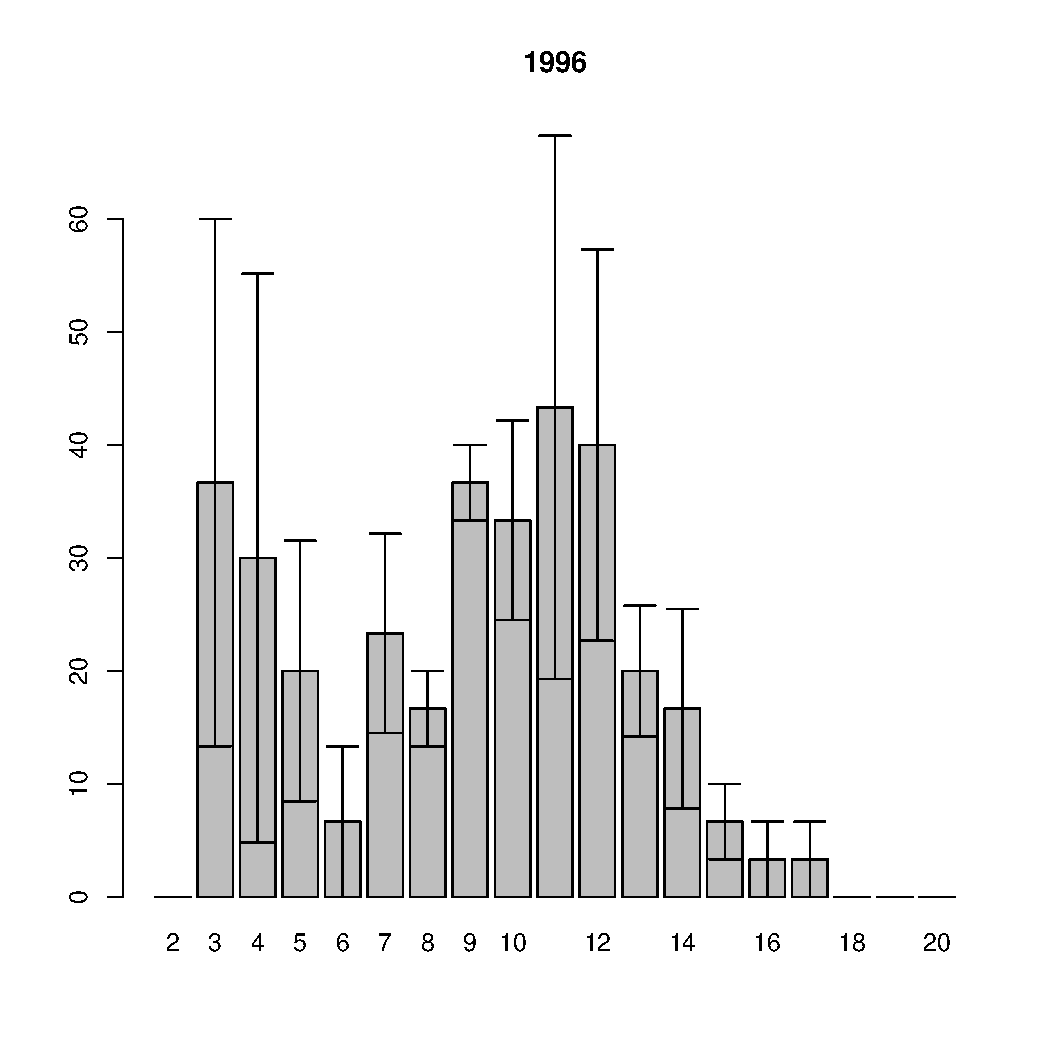
\includegraphics[width=60mm]{../White_Sea/Estuatiy_Luvenga/sizestr2_1996_.pdf}
	\end{center}
	\end{minipage}
	%
	\hfil %Это пружинка отодвигающая рисунки друг от друга
	%
	\begin{minipage}[b]{.3\linewidth}
	\begin{center}
	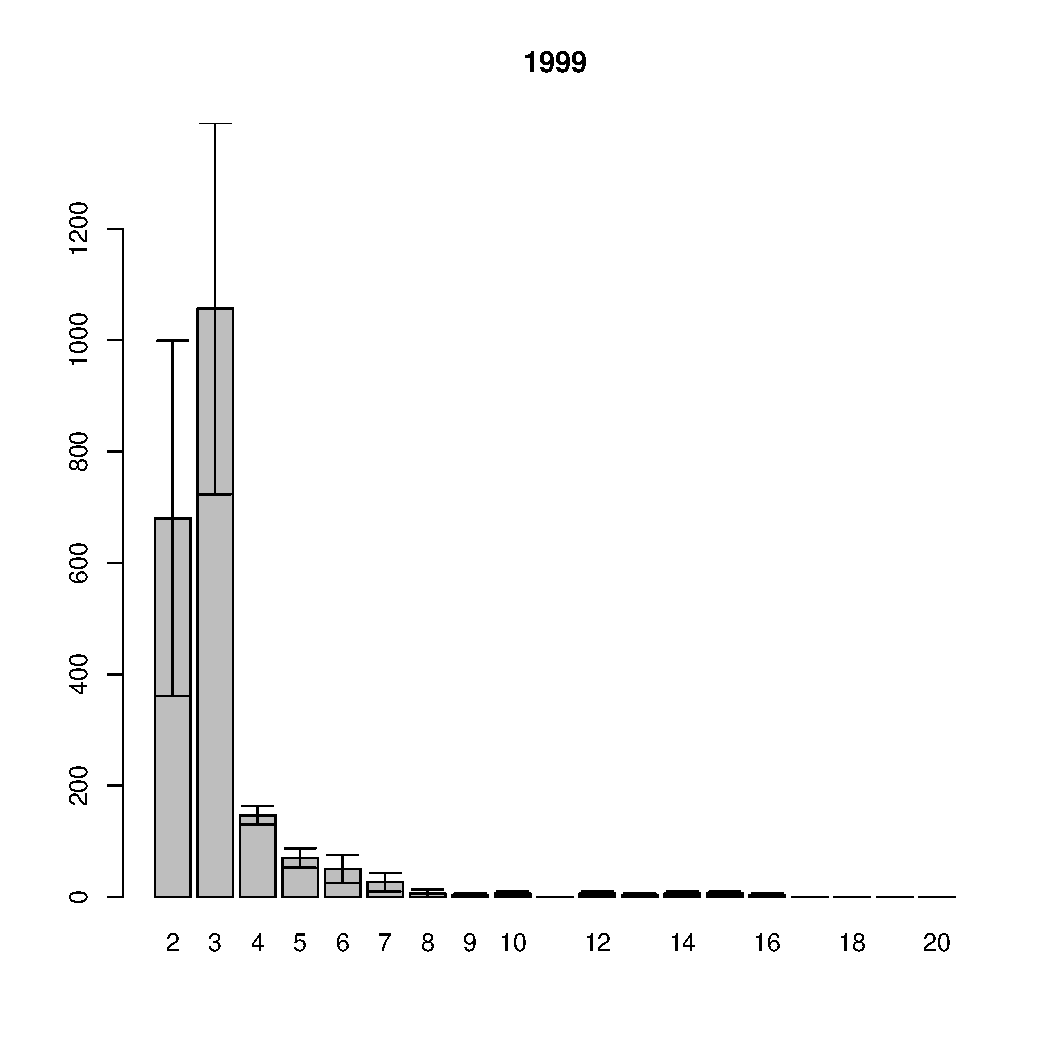
\includegraphics[width=60mm]{../White_Sea/Estuatiy_Luvenga/sizestr2_1999_.pdf}
	\end{center}
	\end{minipage}
	%


	\begin{minipage}[b]{.3\linewidth}
	\begin{center}
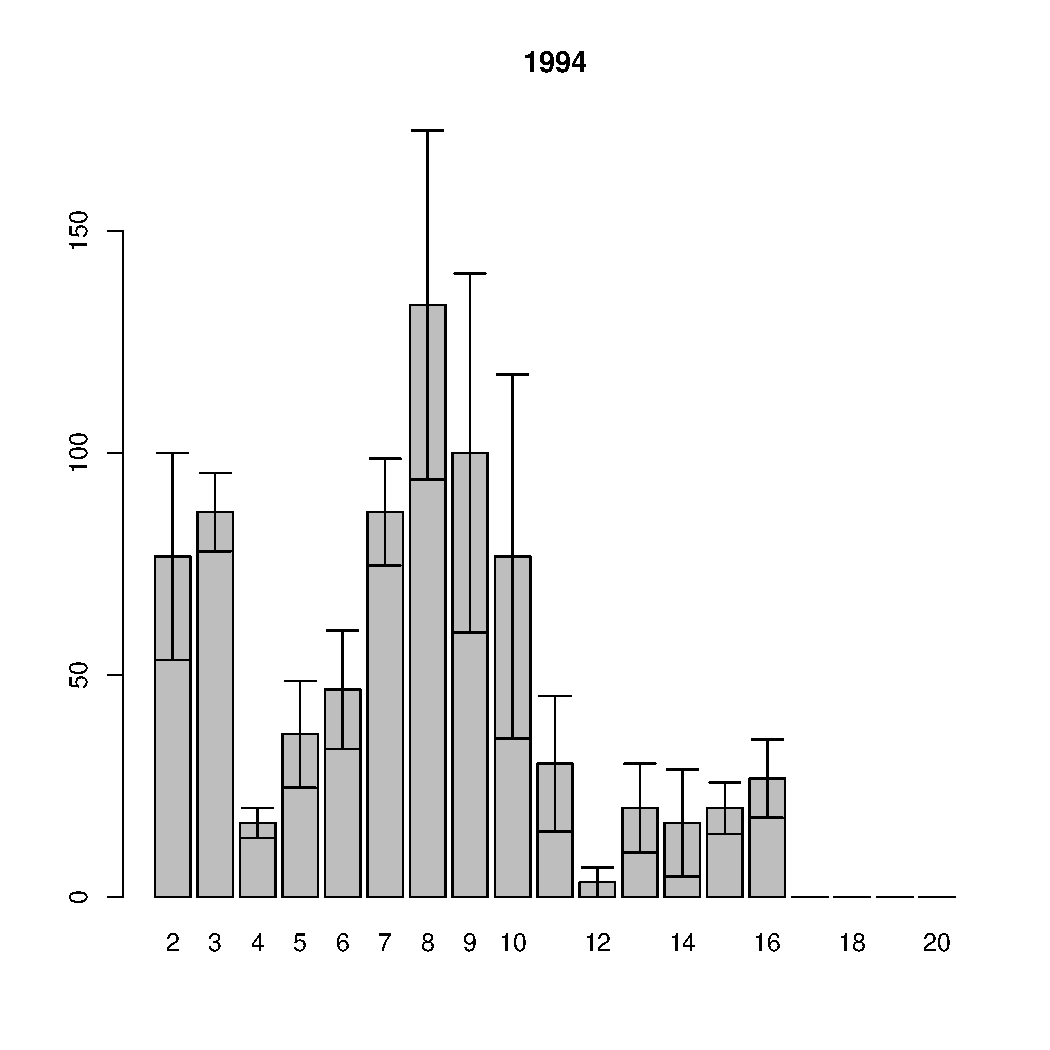
\includegraphics[width=60mm]{../White_Sea/Estuatiy_Luvenga/sizestr2_1994_.pdf}
	\end{center}
	\end{minipage}
	%
	\hfill
	%
	\begin{minipage}[b]{.3\linewidth}
	\begin{center}
	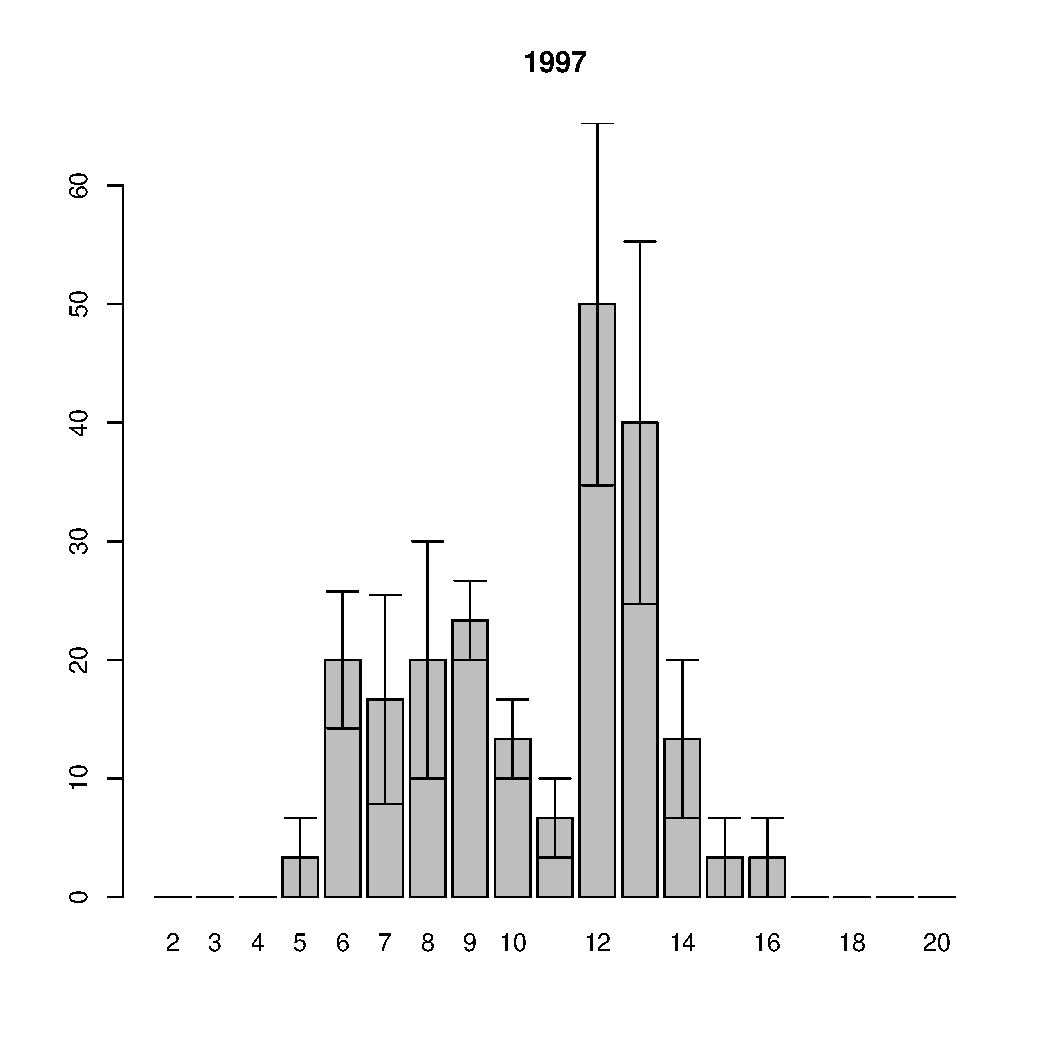
\includegraphics[width=60mm]{../White_Sea/Estuatiy_Luvenga/sizestr2_1997_.pdf}
	\end{center}
	\end{minipage}	
	%
	\hfill
	%
	\begin{minipage}[b]{.3\linewidth}
	\begin{center}
	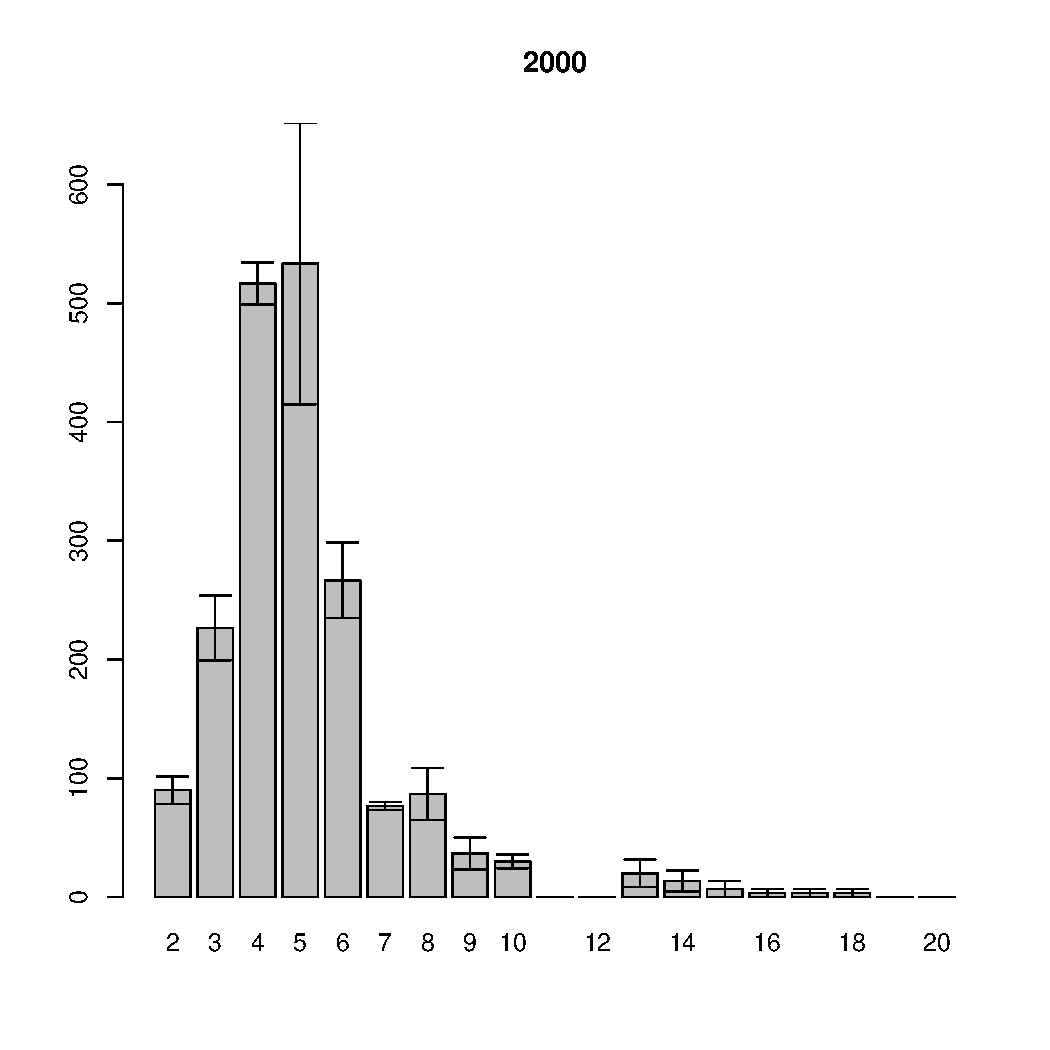
\includegraphics[width=60mm]{../White_Sea/Estuatiy_Luvenga/sizestr2_2000_.pdf}
	\end{center}
	\end{minipage}
%\smallskip
	%
	\caption{Размерная структура {\it Macoma balthica} в СГЛ эстуария р. Лувеньги}
	\label{ris:size_str_estuary_Luv}
	\end{figure}

%%%% вторая страница картинок с РС
	\begin{figure}[hp]

	\begin{minipage}[b]{.3\linewidth}
	\begin{center}
	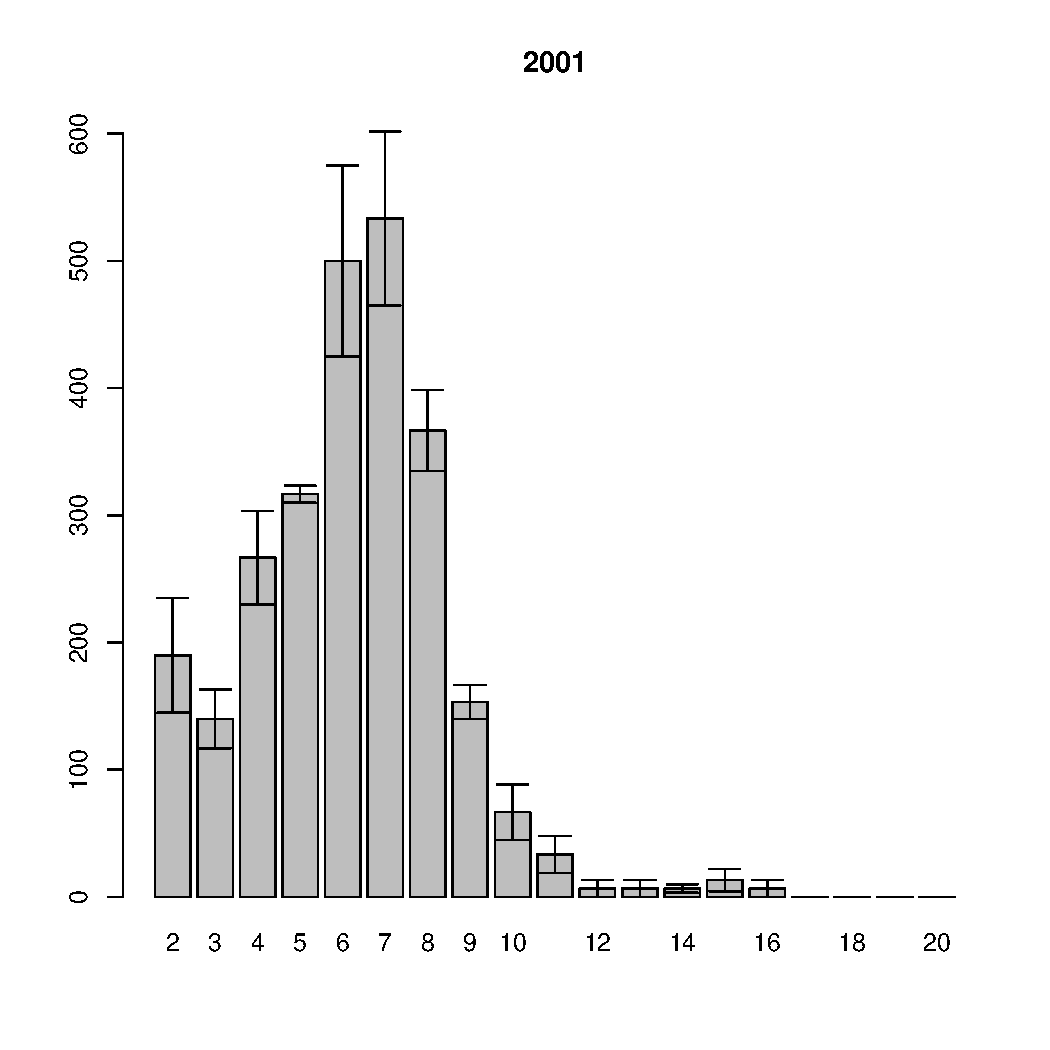
\includegraphics[width=60mm]{../White_Sea/Estuatiy_Luvenga/sizestr2_2001_.pdf}
	\end{center}
	\end{minipage}
	%
	\hfill
	%
	\begin{minipage}[b]{.3\linewidth}
	\begin{center}
	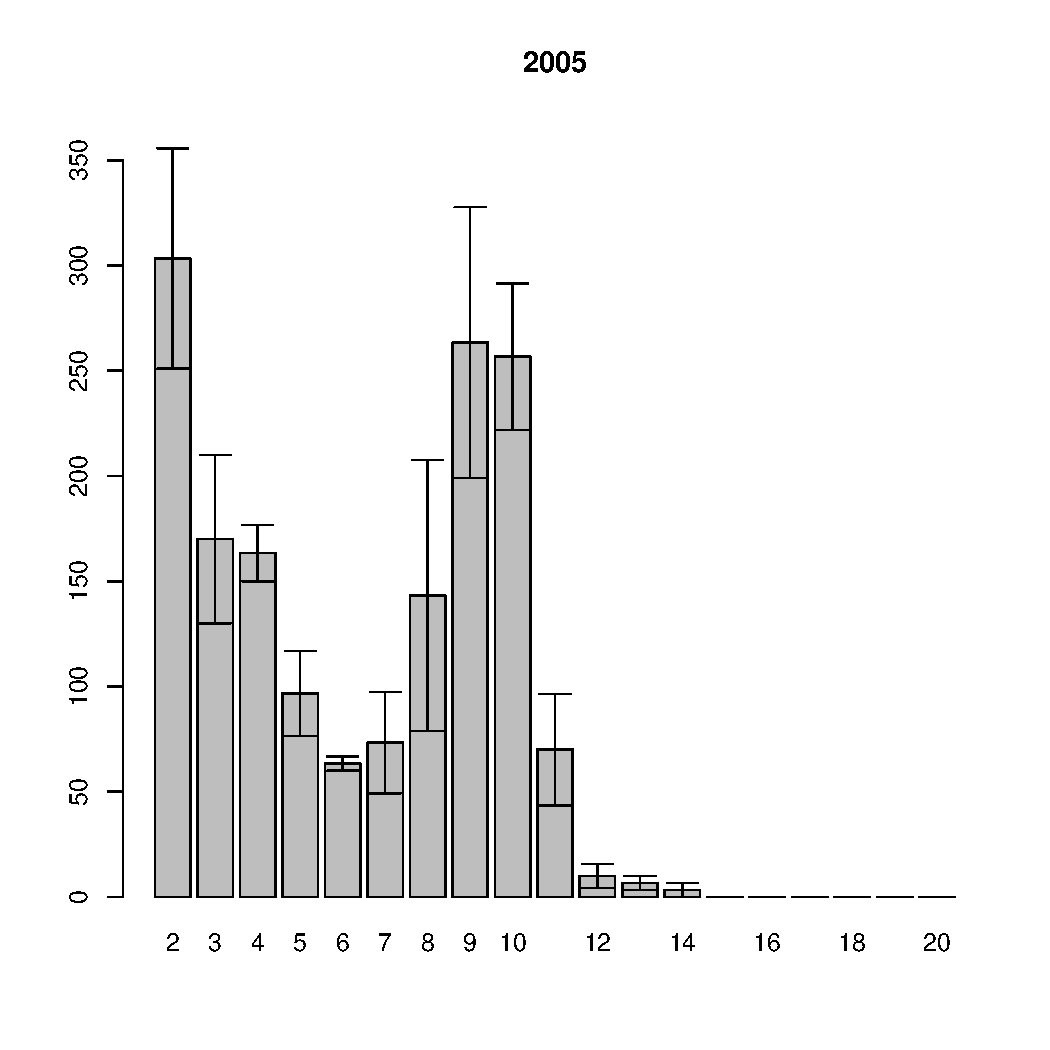
\includegraphics[width=60mm]{../White_Sea/Estuatiy_Luvenga/sizestr2_2005_.pdf}
	\end{center}
	\end{minipage}
	%
	\hfill
	%
	\begin{minipage}[b]{.3\linewidth}
	\begin{center}
	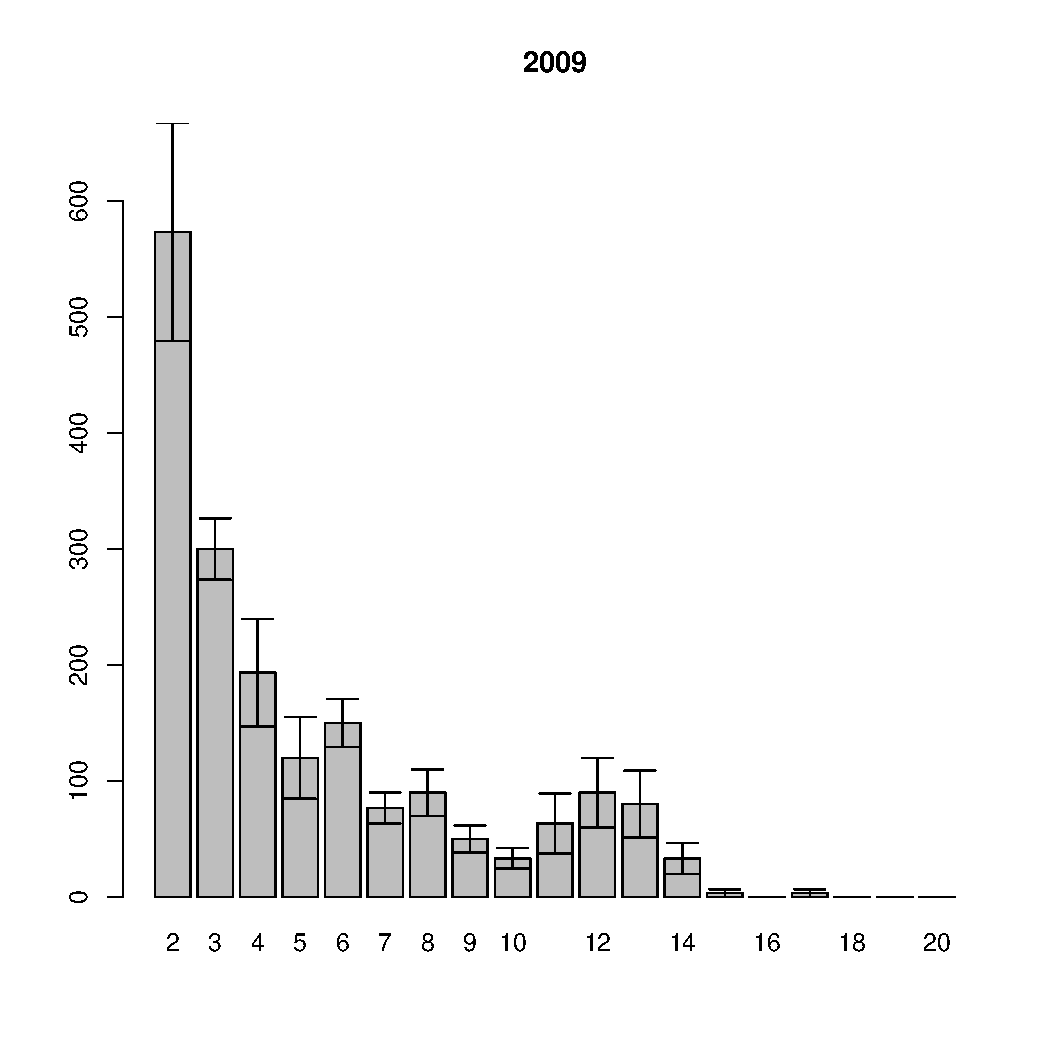
\includegraphics[width=60mm]{../White_Sea/Estuatiy_Luvenga/sizestr2_2009_.pdf}
	\end{center}
	\end{minipage}
	%
	%
	\begin{minipage}[b]{.3\linewidth}
	\begin{center}
	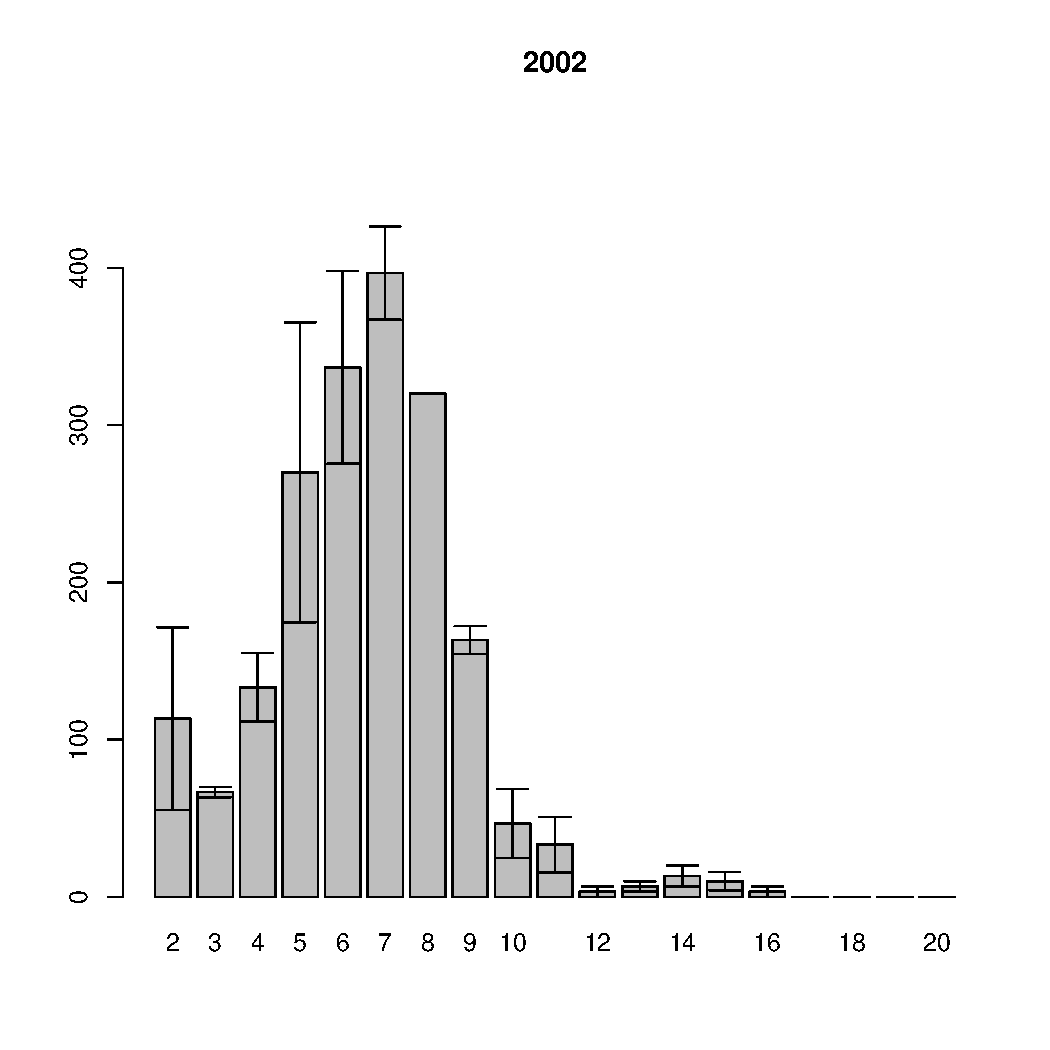
\includegraphics[width=60mm]{../White_Sea/Estuatiy_Luvenga/sizestr2_2002_.pdf}
	\end{center}
	\end{minipage}
	%
	\hfill	
	%
	\begin{minipage}[b]{.3\linewidth}
	\begin{center}
	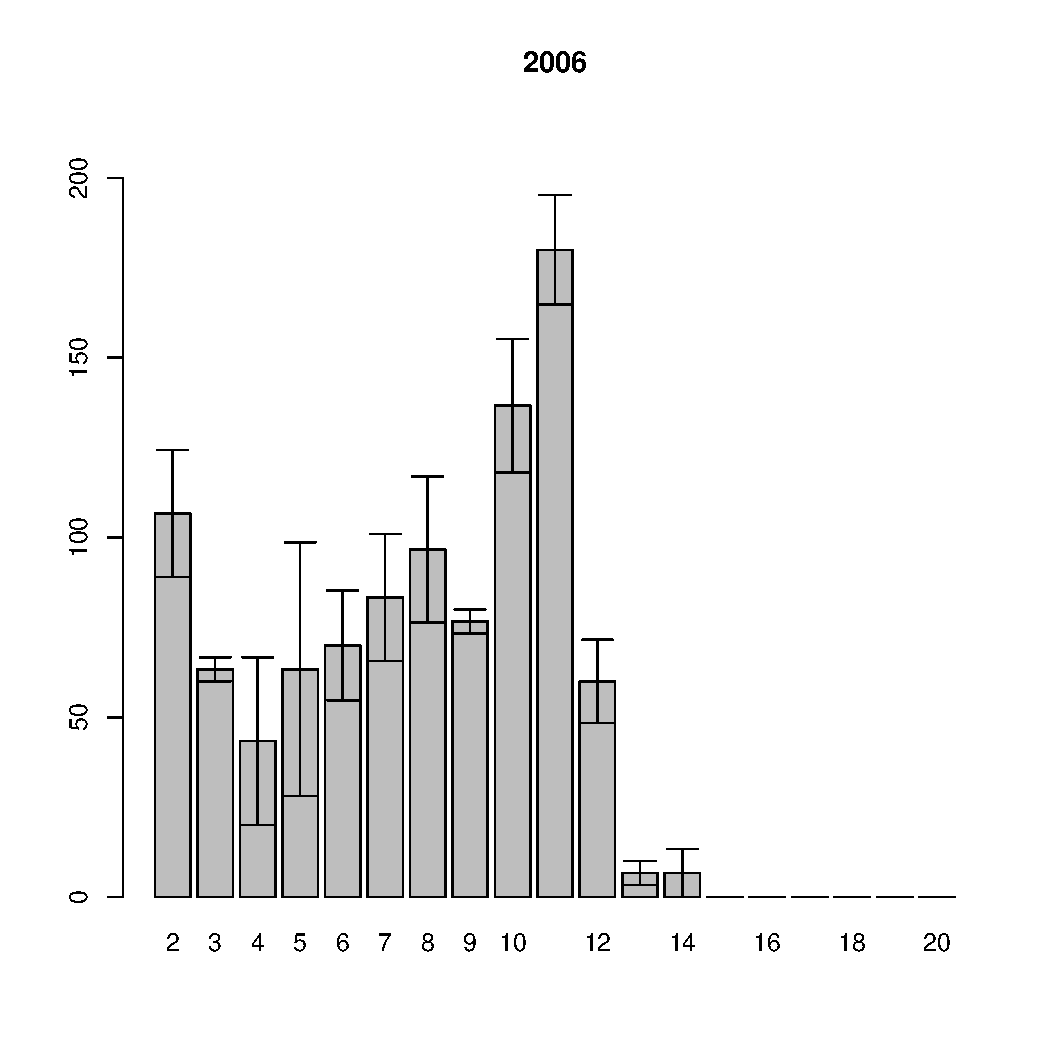
\includegraphics[width=60mm]{../White_Sea/Estuatiy_Luvenga/sizestr2_2006_.pdf}
	\end{center}
	\end{minipage}
	%
	\hfill
	%
	\begin{minipage}[b]{.3\linewidth}
	\begin{center}
	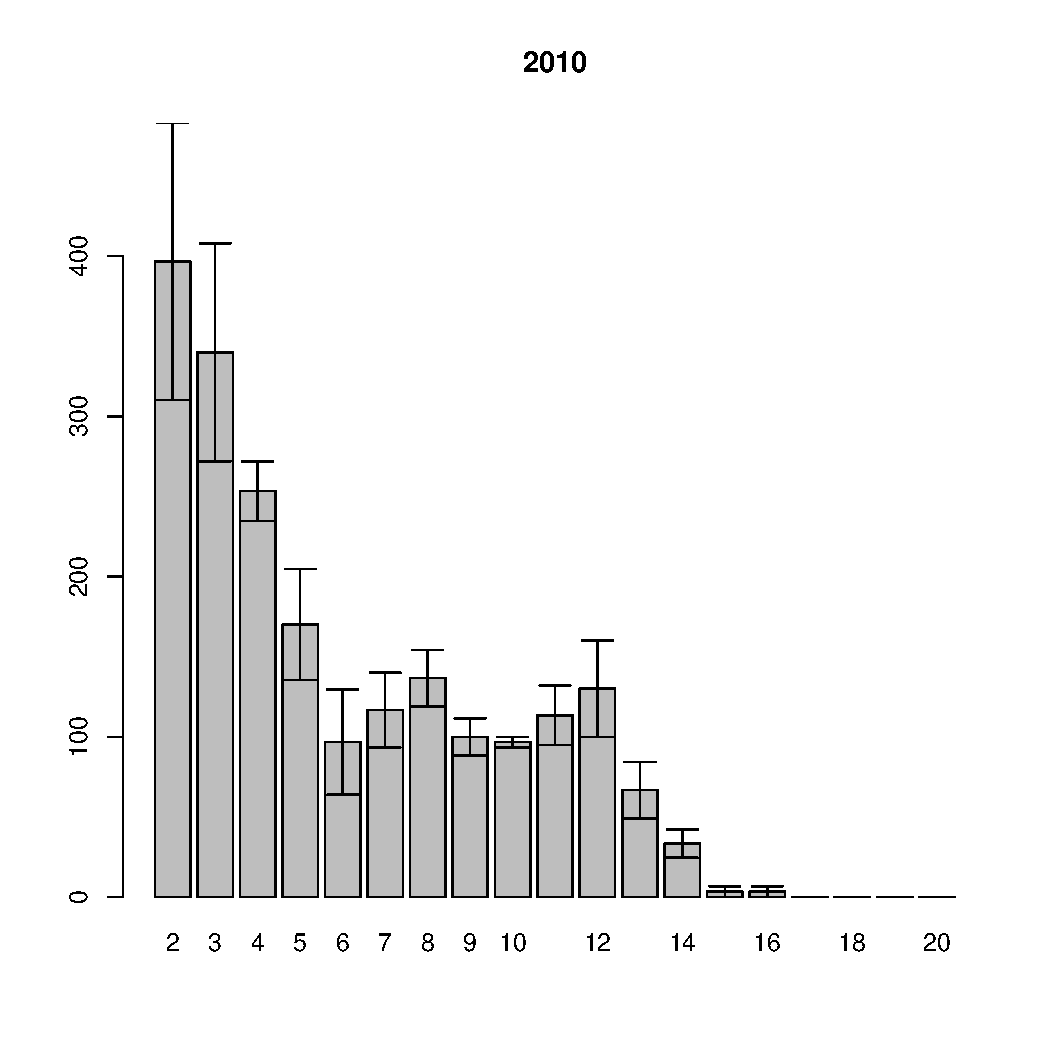
\includegraphics[width=60mm]{../White_Sea/Estuatiy_Luvenga/sizestr2_2010_.pdf}
	\end{center}
	\end{minipage}
	%
	%
	\begin{minipage}[b]{.3\linewidth}
	\begin{center}
	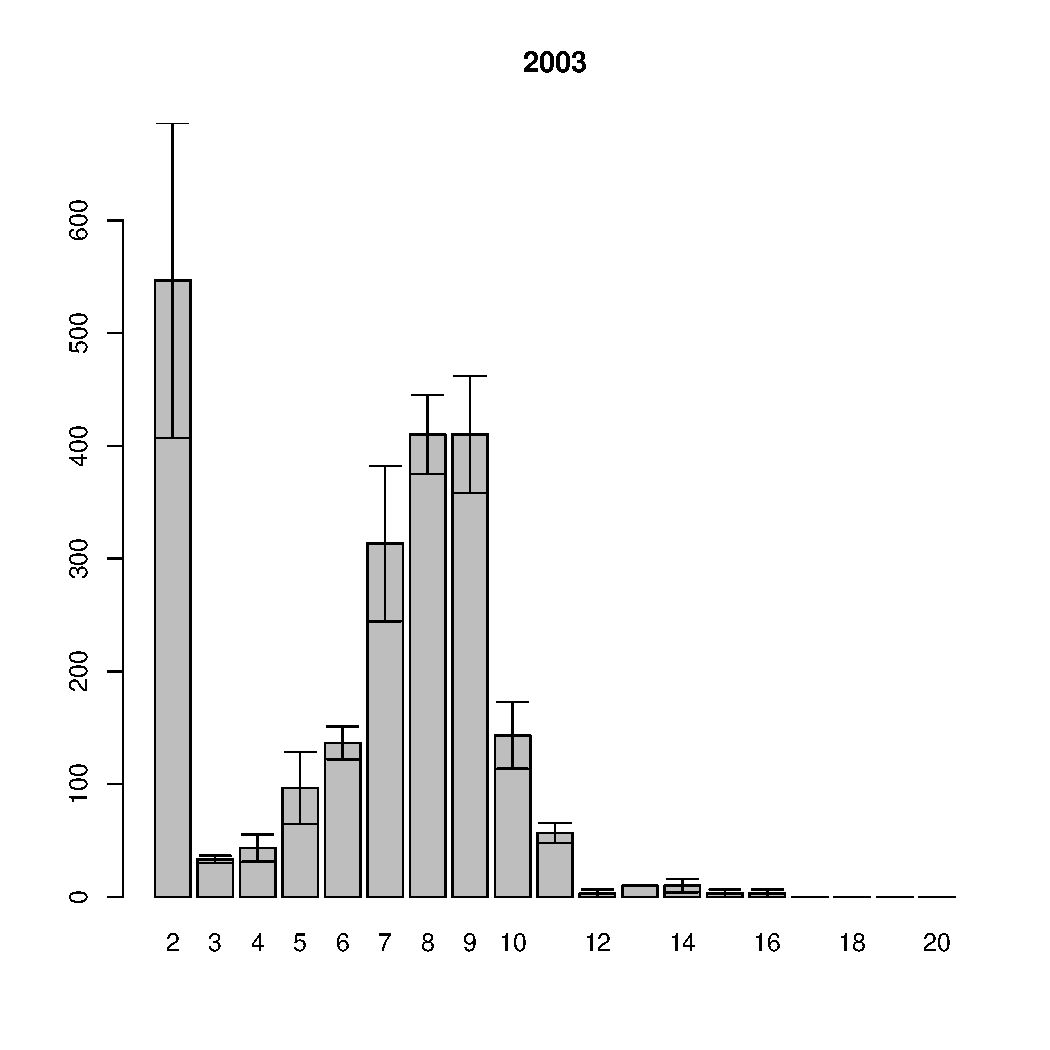
\includegraphics[width=60mm]{../White_Sea/Estuatiy_Luvenga/sizestr2_2003_.pdf}
	\end{center}
	\end{minipage}
	%
	\hfill
	%
	\begin{minipage}[b]{.3\linewidth}
	\begin{center}
	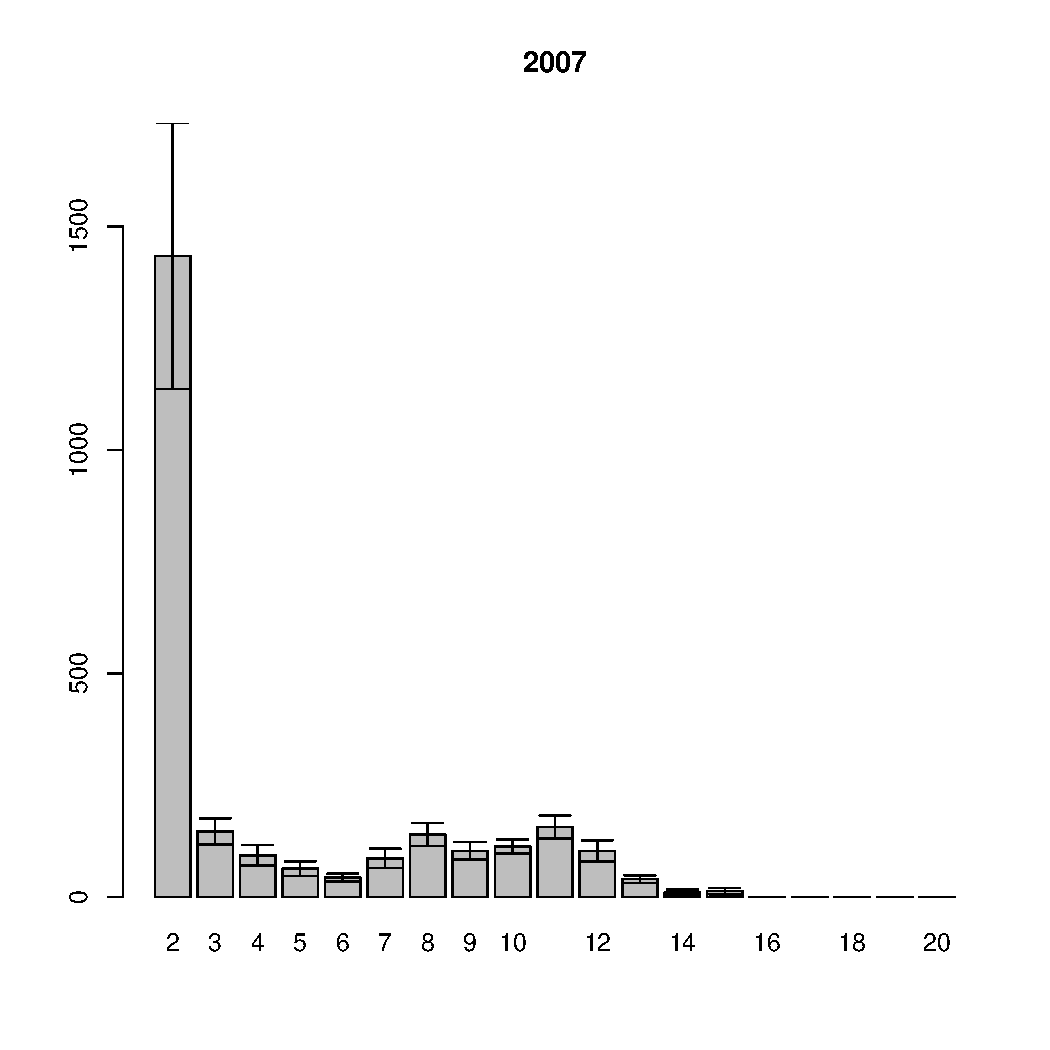
\includegraphics[width=60mm]{../White_Sea/Estuatiy_Luvenga/sizestr2_2007_.pdf}
	\end{center}
	\end{minipage}
	%
	\hfill
	%
	\begin{minipage}[b]{.3\linewidth}
	\begin{center}
	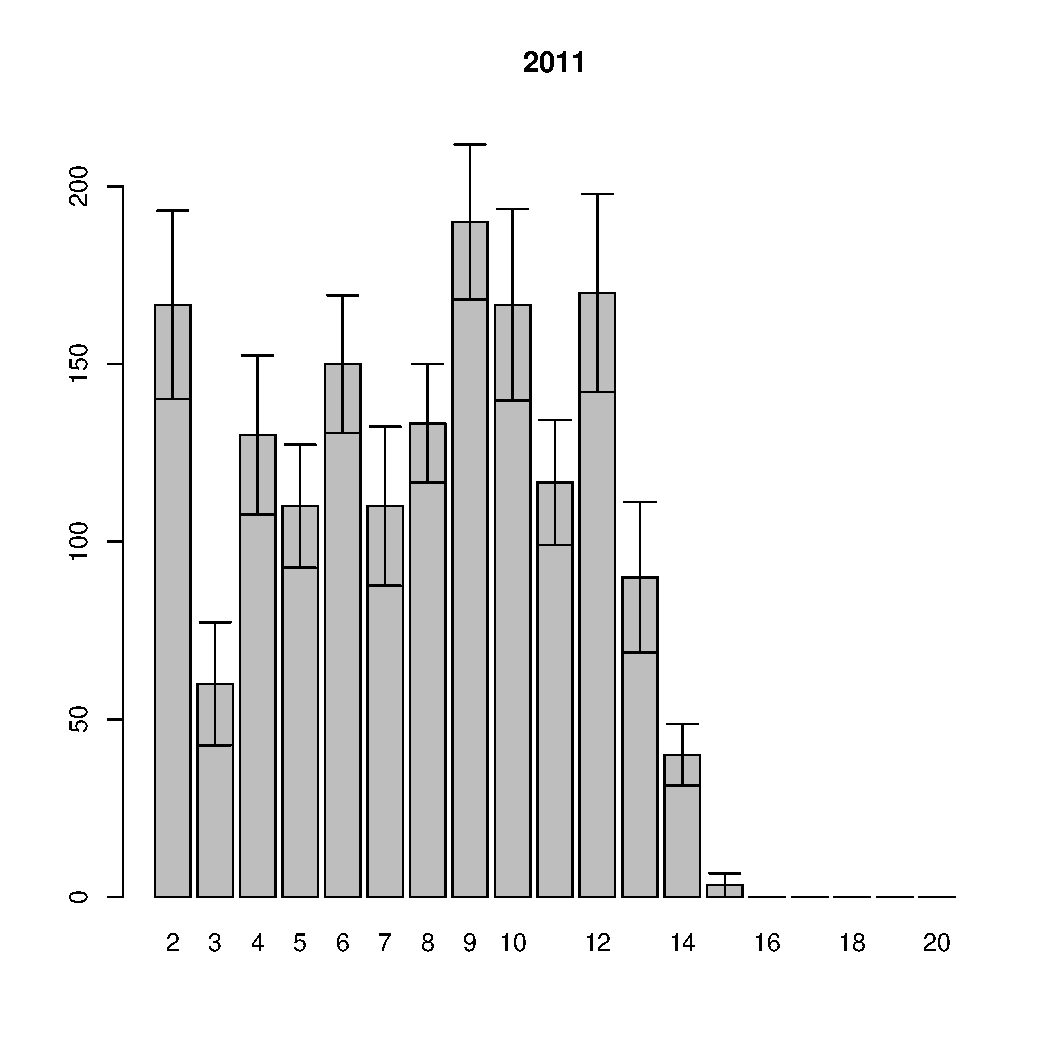
\includegraphics[width=60mm]{../White_Sea/Estuatiy_Luvenga/sizestr2_2011_.pdf}
	\end{center}
	\end{minipage}
	%

	\begin{minipage}[b]{.3\linewidth}
	\begin{center}
	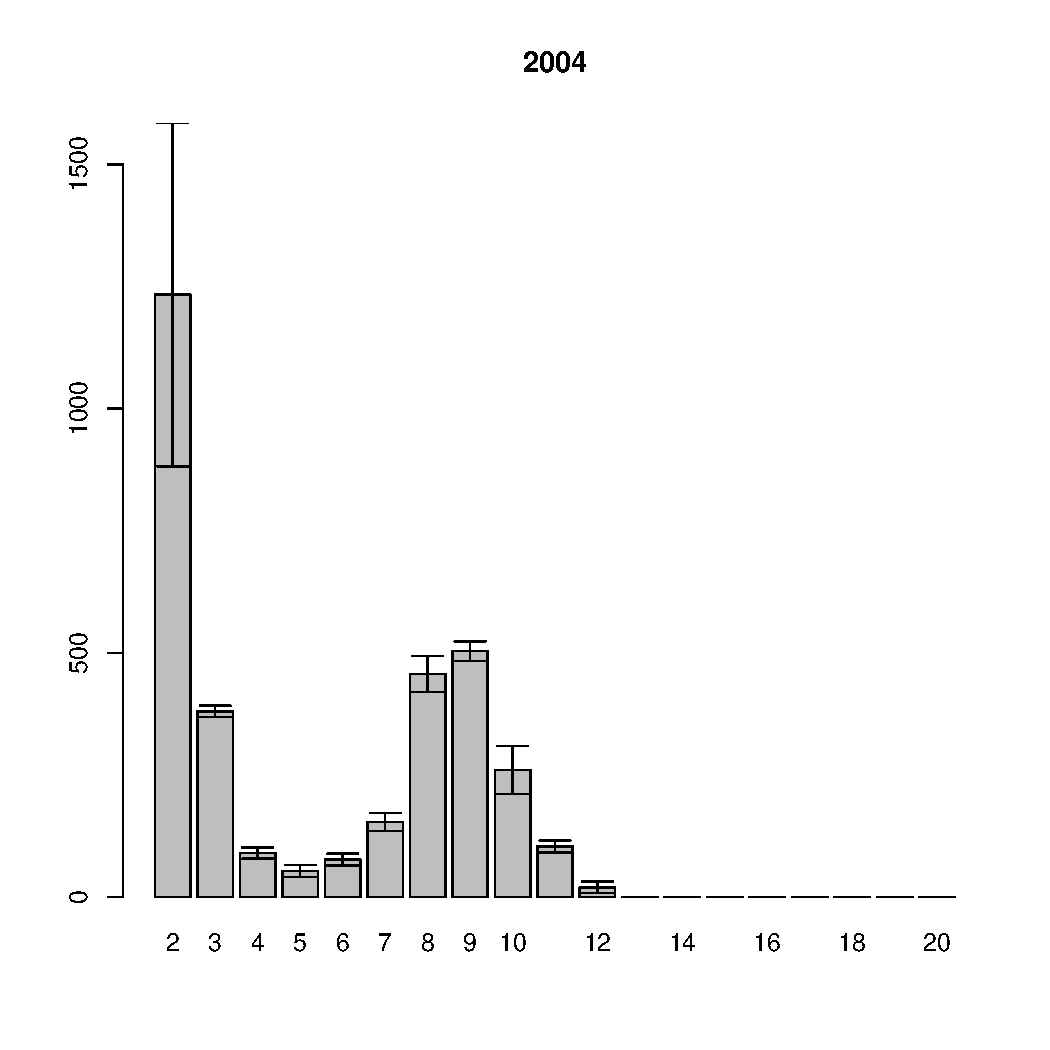
\includegraphics[width=60mm]{../White_Sea/Estuatiy_Luvenga/sizestr2_2004_.pdf}
	\end{center}
	\end{minipage}
	%
	\hfill
	%
	\begin{minipage}[b]{.3\linewidth}
	\begin{center}
	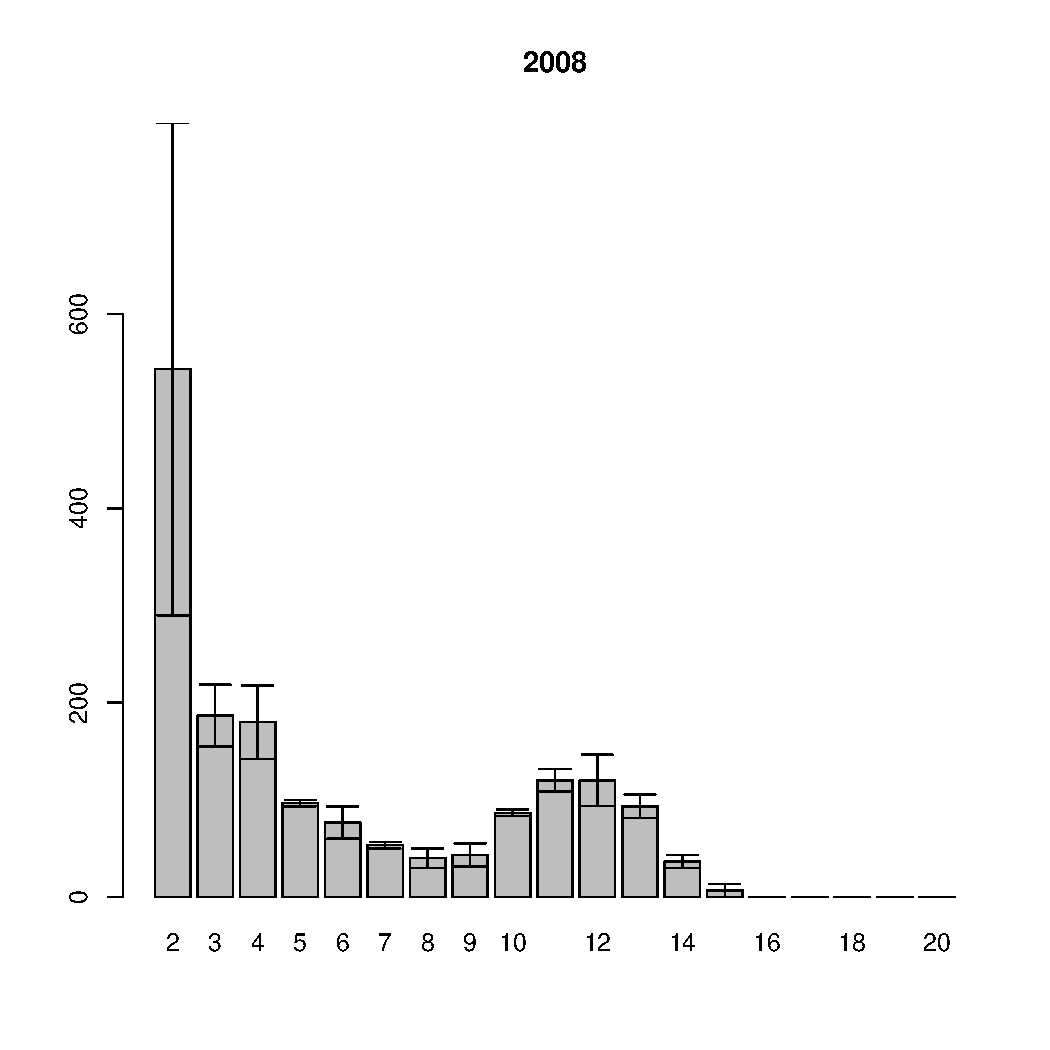
\includegraphics[width=60mm]{../White_Sea/Estuatiy_Luvenga/sizestr2_2008_.pdf}
	\end{center}
	\end{minipage}
	%
	\hfill
	%
	\begin{minipage}[b]{.3\linewidth}
	\begin{center}
	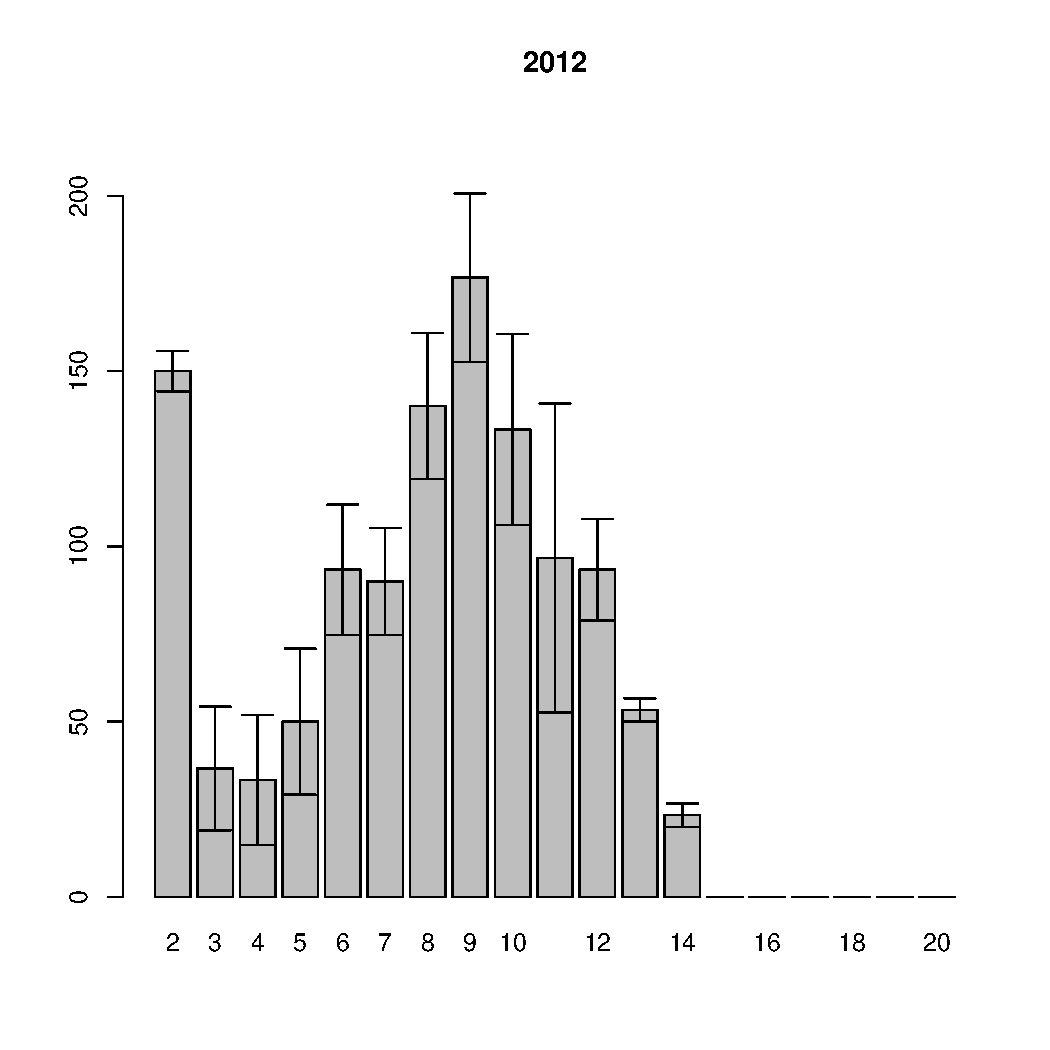
\includegraphics[width=60mm]{../White_Sea/Estuatiy_Luvenga/sizestr2_2012_.pdf}
	\end{center}
	\end{minipage}
	\begin{center}
	Рис. \ref{ris:size_str_estuary_Luv} (продолжение). Размерная структура {\it Macoma balthica} в СГЛ эстуария р. Лувеньги
	\end{center}
	\end{figure}


%%%%%%%%%%%%%%%%%%%%%%%%%%%%%%
%Горелый верх
	\begin{figure}[hp]

	\begin{minipage}[b]{.3\linewidth}
	\begin{center}
	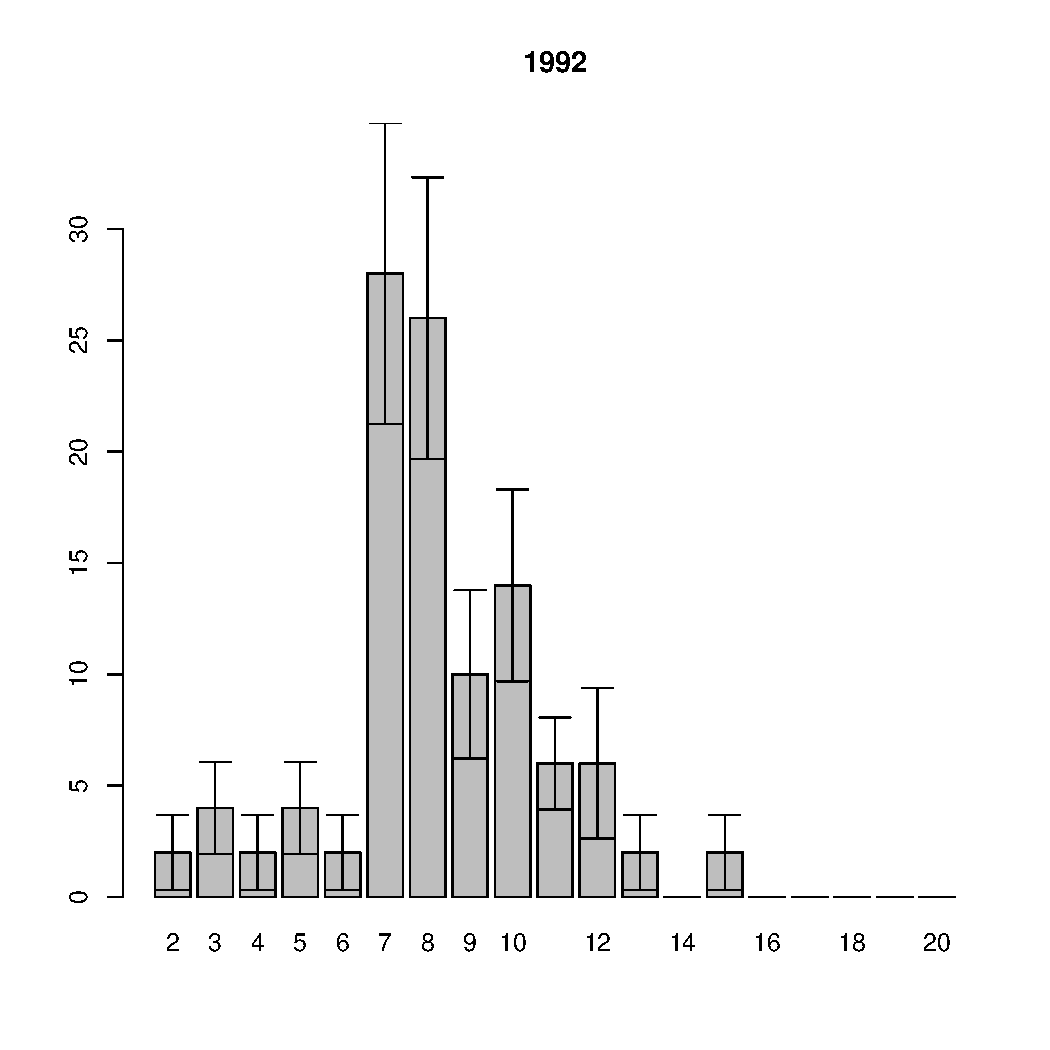
\includegraphics[width=60mm]{../White_Sea/Luvenga_Goreliy/high2_1992_.pdf}	
	\end{center}
	\end{minipage}
	%
	\hfil %Это пружинка отодвигающая рисунки друг от друга
	%
	\begin{minipage}[b]{.3\linewidth}
	\begin{center}
	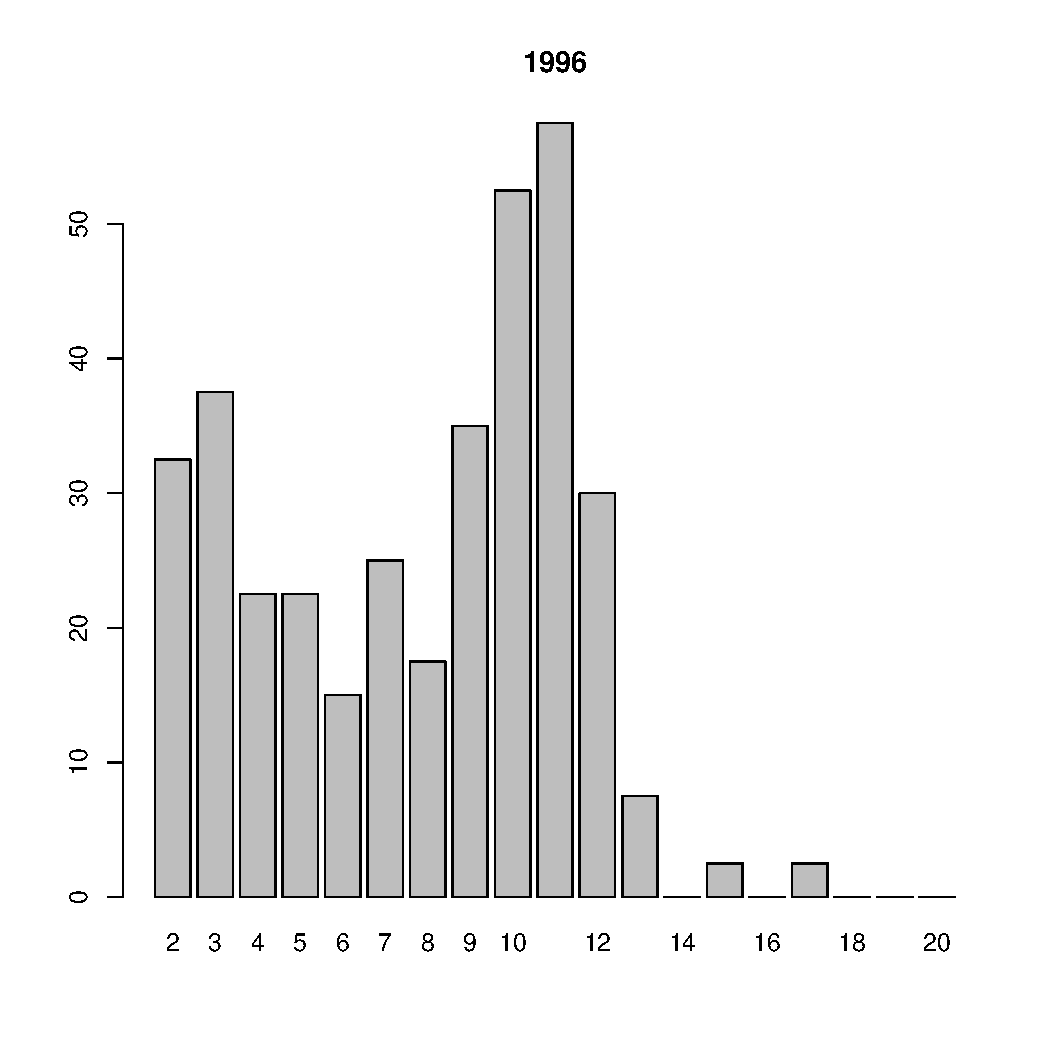
\includegraphics[width=60mm]{../White_Sea/Luvenga_Goreliy/high2_1996_.pdf}
	\end{center}
	\end{minipage}
	%
	\hfil %Это пружинка отодвигающая рисунки друг от друга
	%
	\begin{minipage}[b]{.3\linewidth}
	\begin{center}
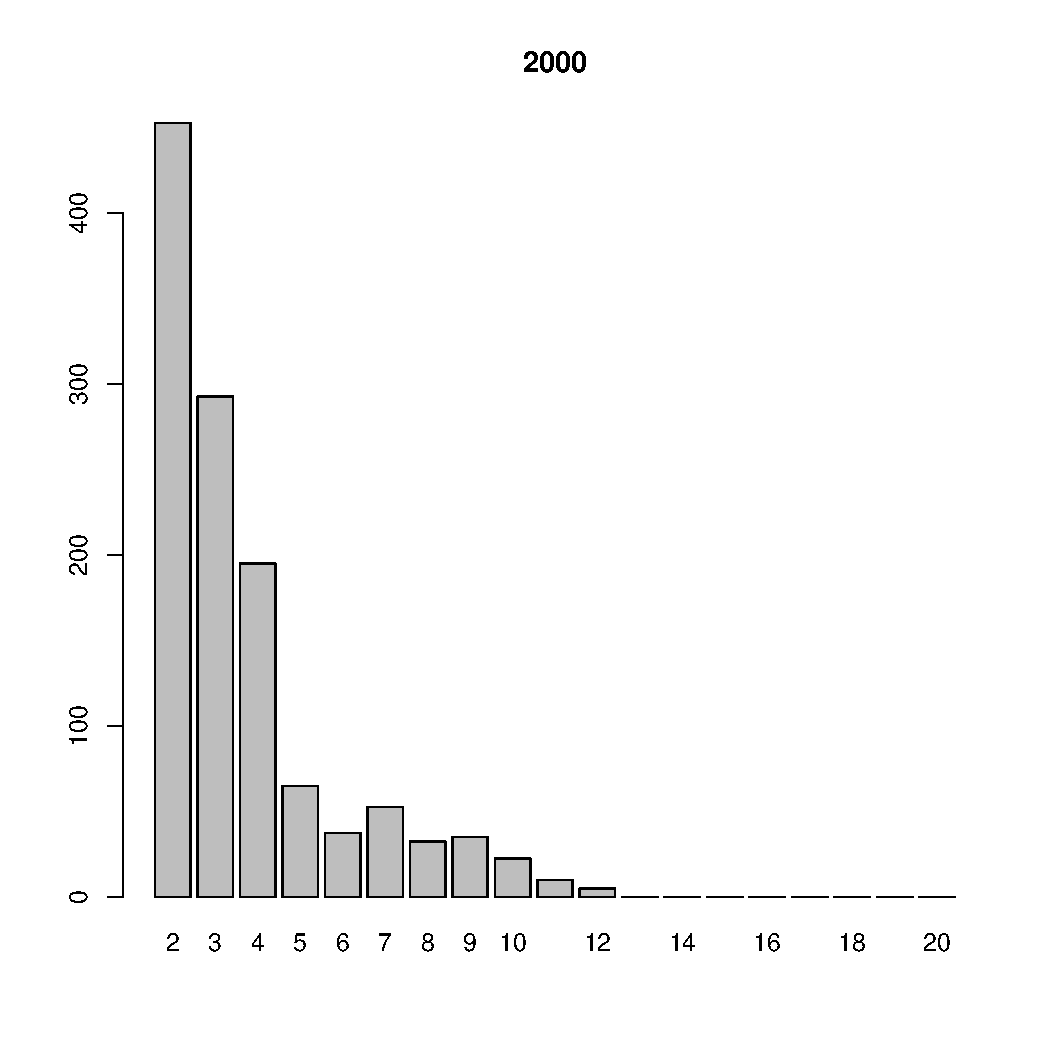
\includegraphics[width=60mm]{../White_Sea/Luvenga_Goreliy/high2_2000_.pdf}
	\end{center}
	\end{minipage}
	%
	\begin{minipage}[b]{.3\linewidth}
	\begin{center}
	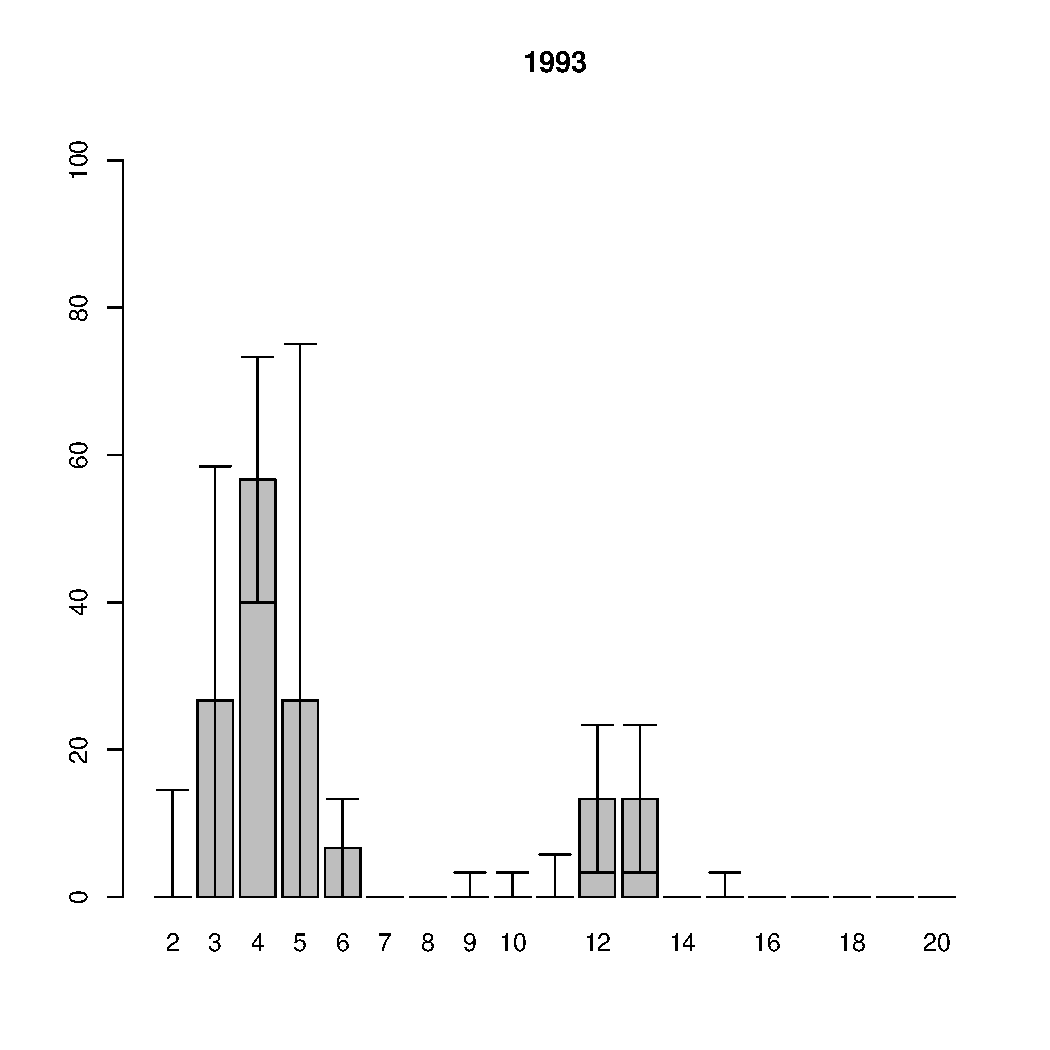
\includegraphics[width=60mm]{../White_Sea/Luvenga_Goreliy/high2_1993_.pdf}
	\end{center}
	\end{minipage}
	%
	\hfil %Это пружинка отодвигающая рисунки друг от друга
	%
	\begin{minipage}[b]{.3\linewidth}
	\begin{center}
	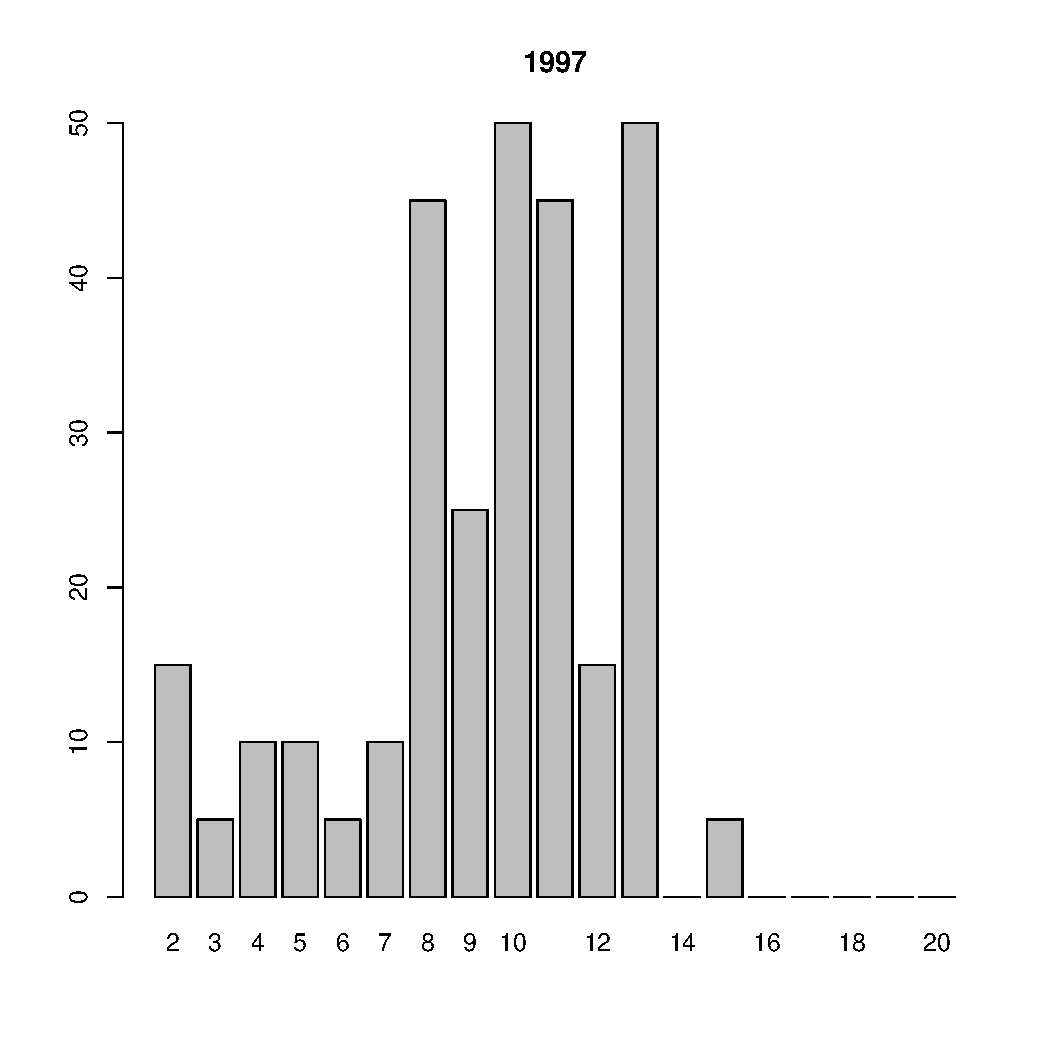
\includegraphics[width=60mm]{../White_Sea/Luvenga_Goreliy/high2_1997_.pdf}
	\end{center}
	\end{minipage}
	%
	\hfil %Это пружинка отодвигающая рисунки друг от друга
	%
	\begin{minipage}[b]{.3\linewidth}
	\begin{center}
	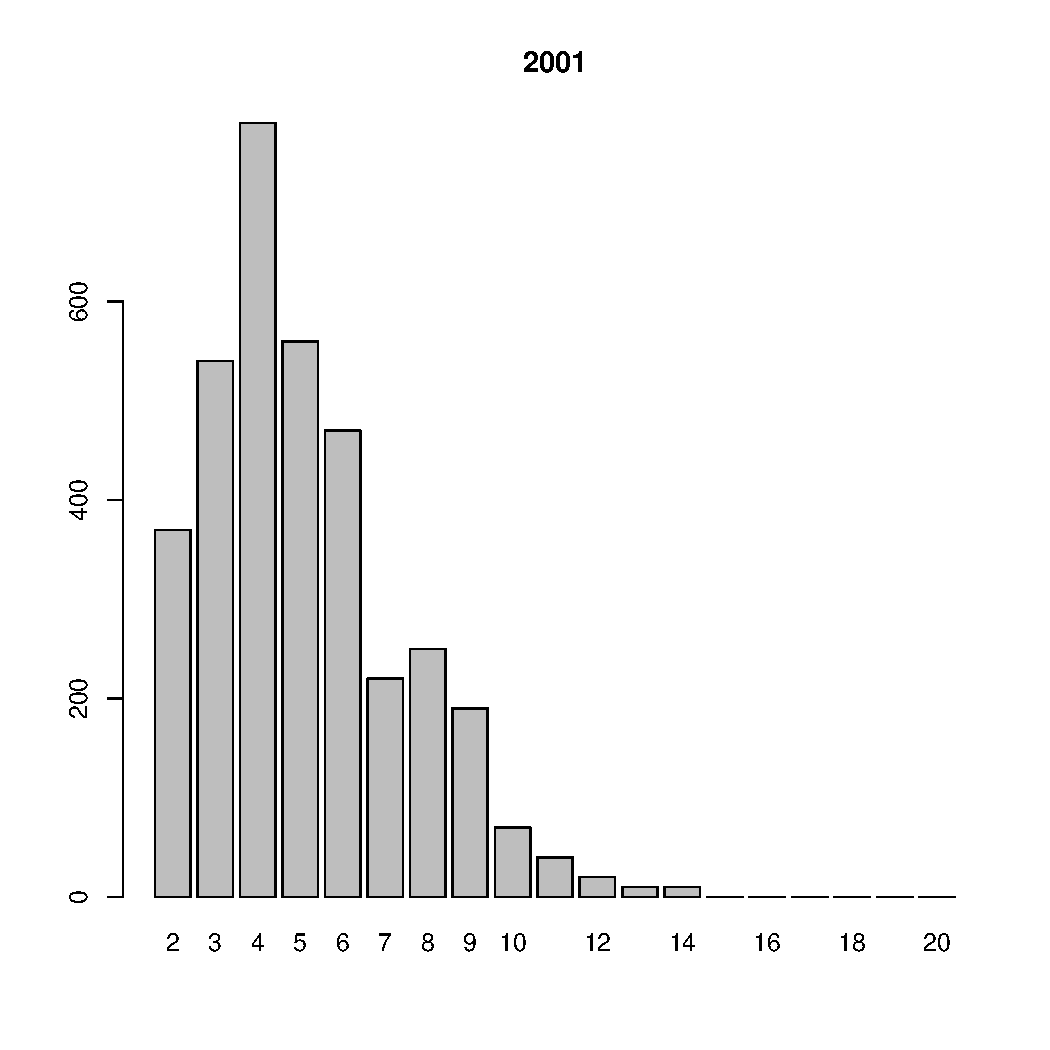
\includegraphics[width=60mm]{../White_Sea/Luvenga_Goreliy/high2_2001_.pdf}
	\end{center}
	\end{minipage}
	%


	\begin{minipage}[b]{.3\linewidth}
	\begin{center}
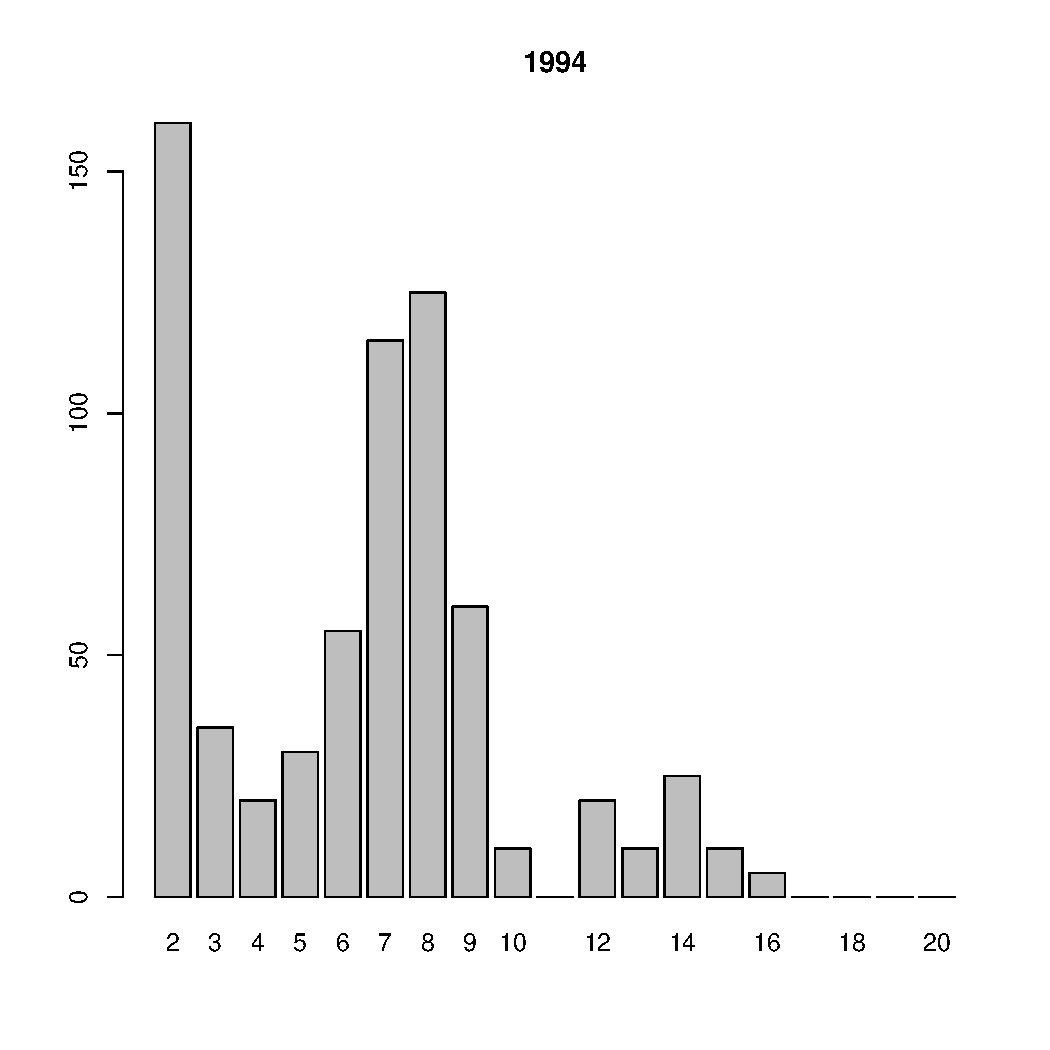
\includegraphics[width=60mm]{../White_Sea/Luvenga_Goreliy/high2_1994_.pdf}
	\end{center}
	\end{minipage}
	%
	\hfill
	%
	\begin{minipage}[b]{.3\linewidth}
	\begin{center}
	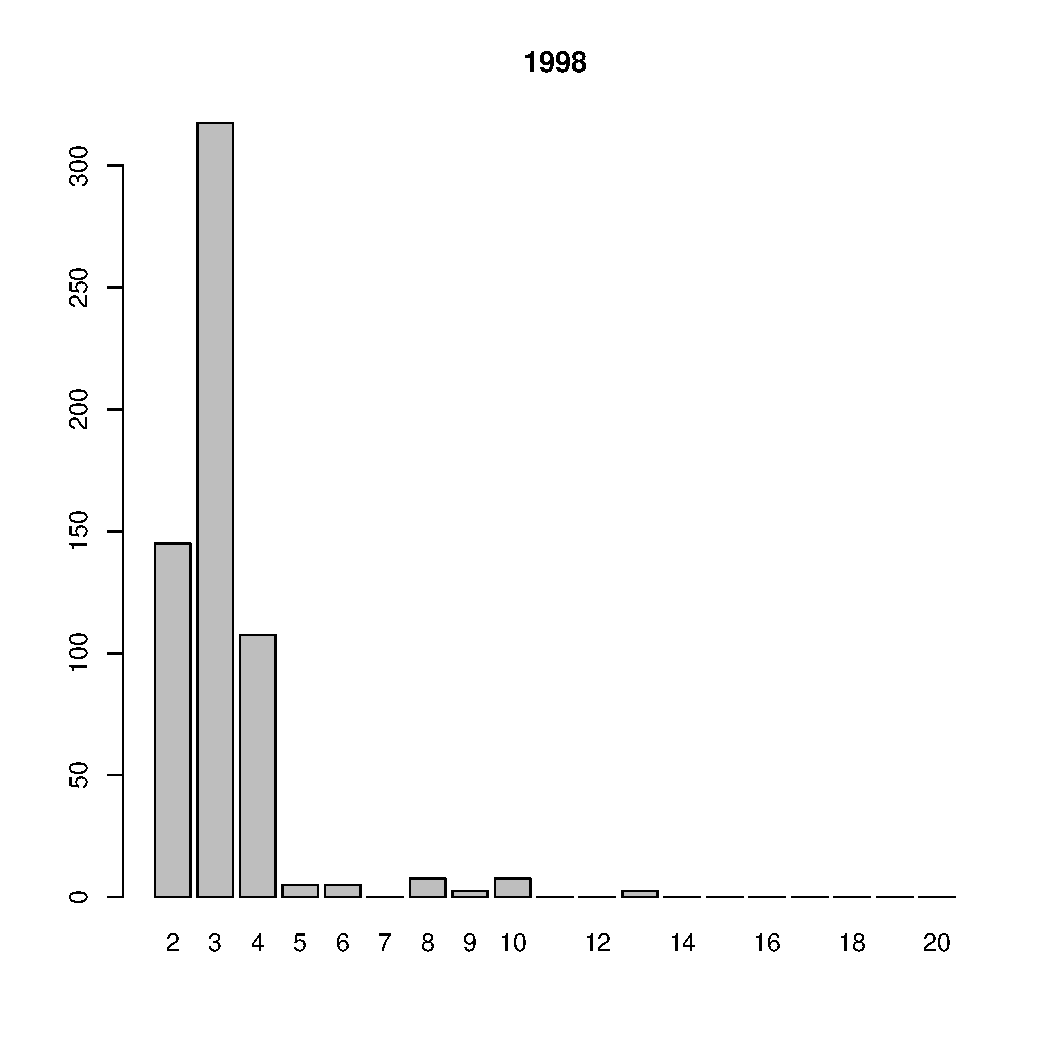
\includegraphics[width=60mm]{../White_Sea/Luvenga_Goreliy/high2_1998_.pdf}
	\end{center}
	\end{minipage}	
	%
	\hfill
	%
	\begin{minipage}[b]{.3\linewidth}
	\begin{center}
	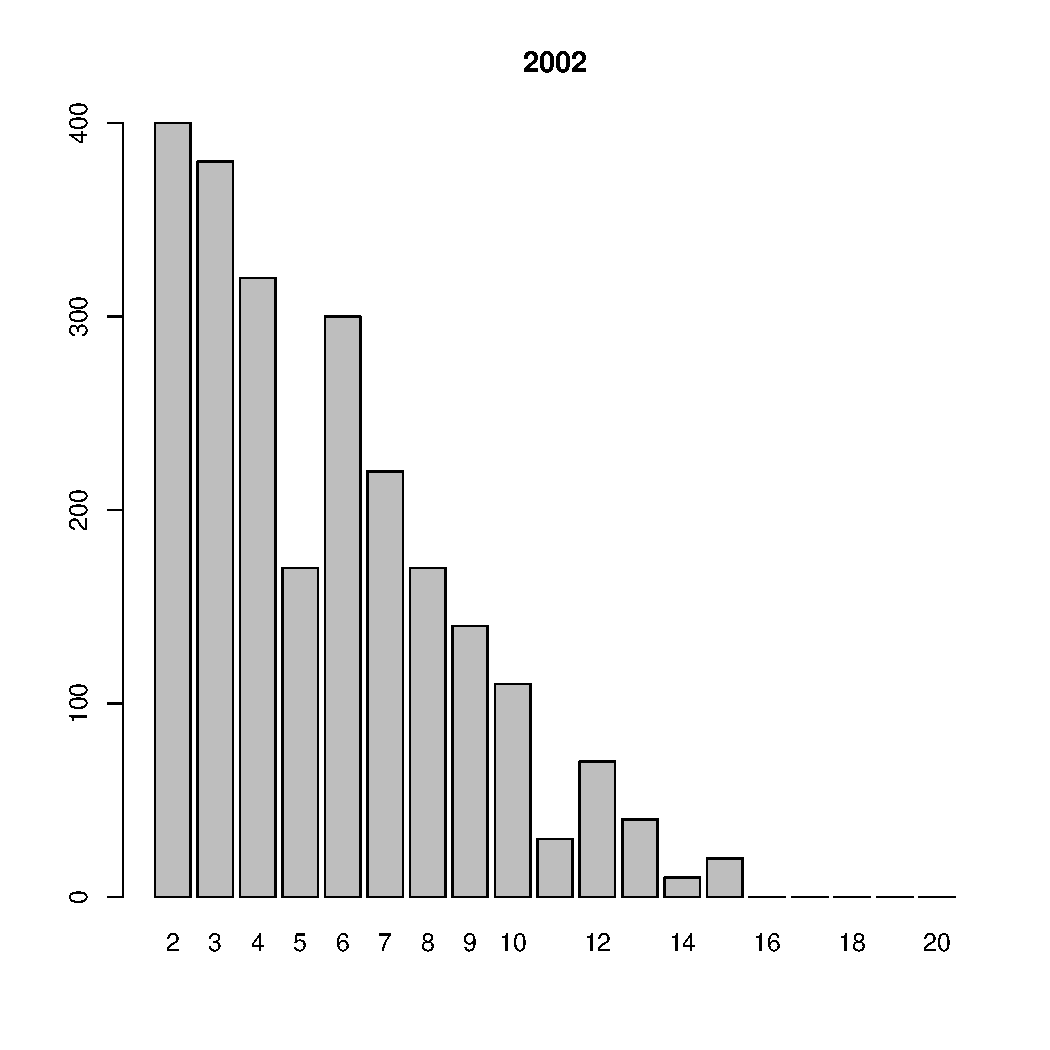
\includegraphics[width=60mm]{../White_Sea/Luvenga_Goreliy/high2_2002_.pdf}
	\end{center}
	\end{minipage}
%\smallskip

	\begin{minipage}[b]{.3\linewidth}
	\begin{center}
	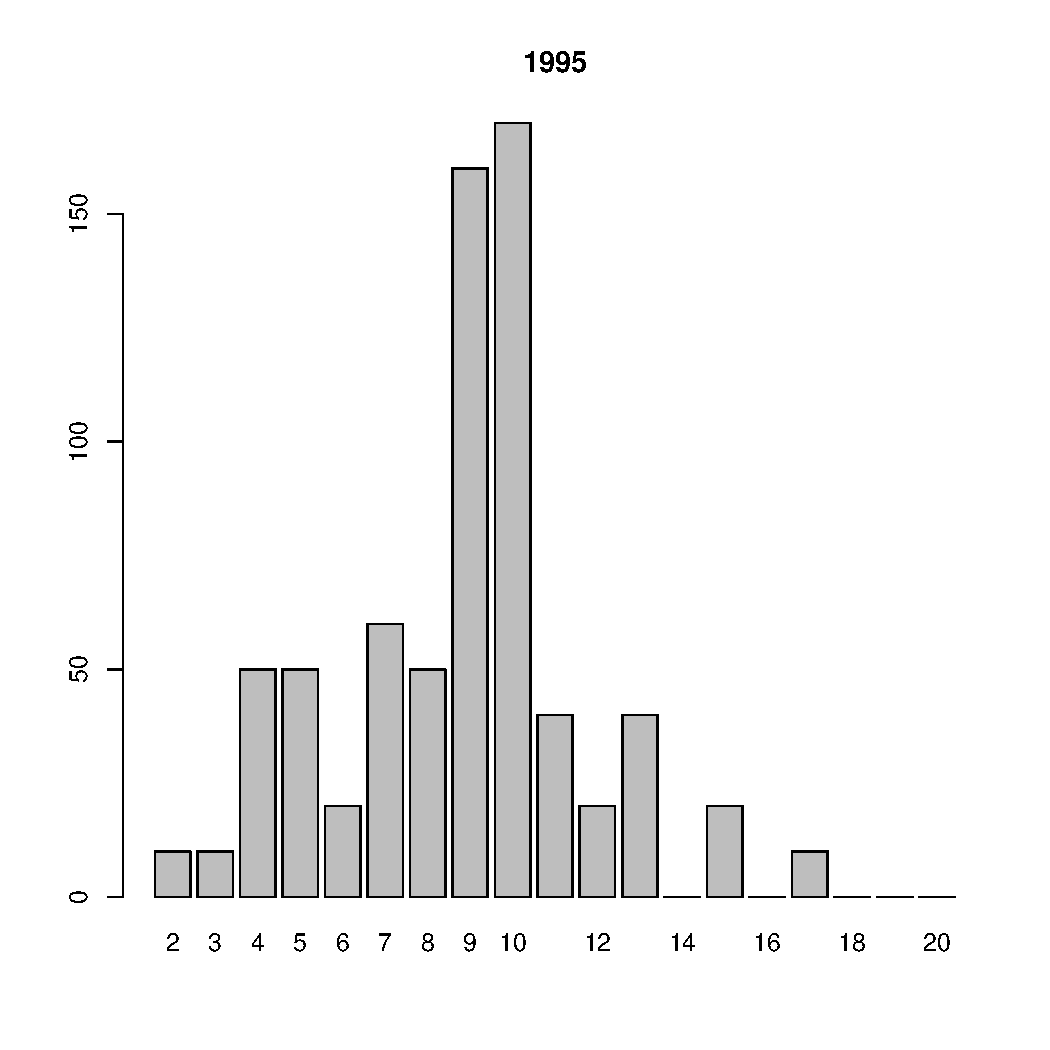
\includegraphics[width=60mm]{../White_Sea/Luvenga_Goreliy/high2_1995_.pdf}
	\end{center}
	\end{minipage}
	%
	\hfill
	%
	\begin{minipage}[b]{.3\linewidth}
	\begin{center}
	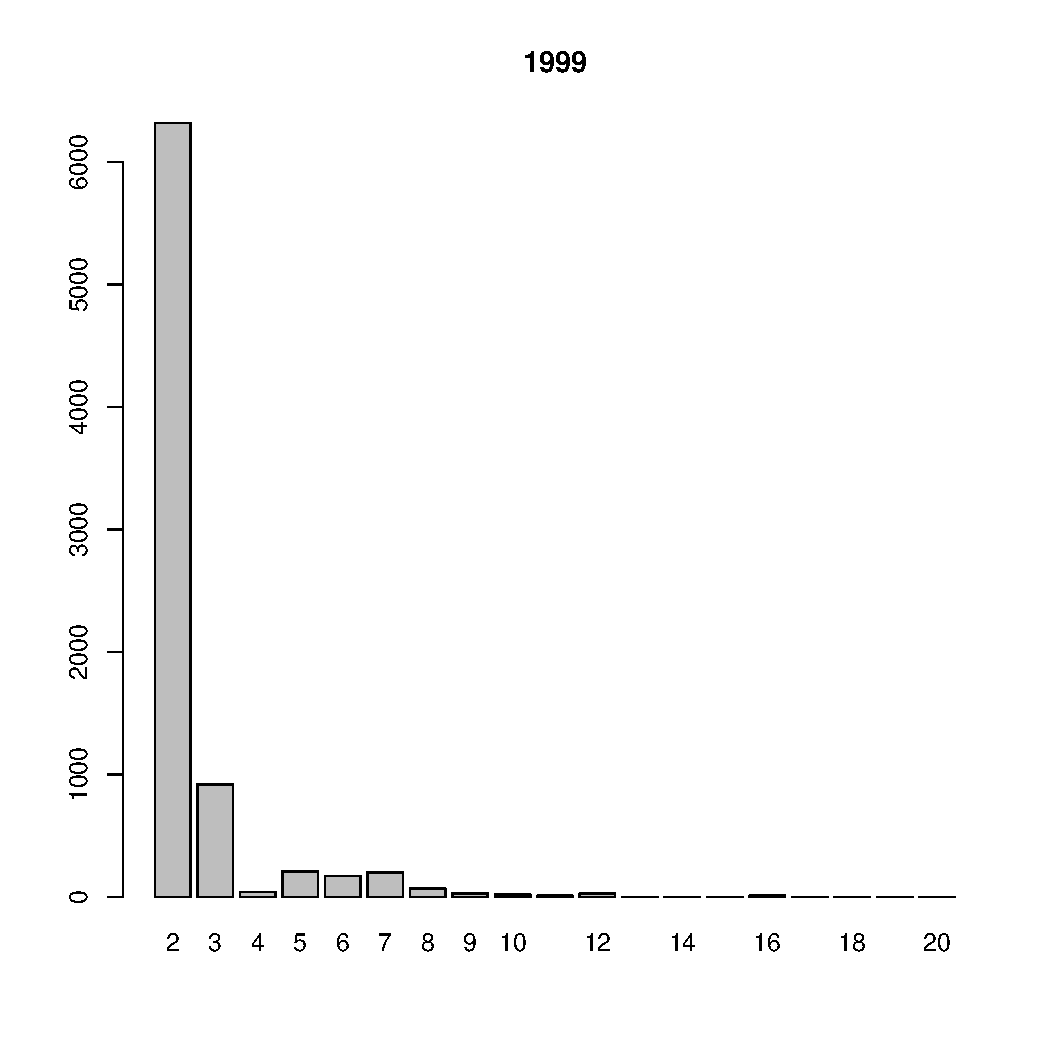
\includegraphics[width=60mm]{../White_Sea/Luvenga_Goreliy/high2_1999_.pdf}
	\end{center}
	\end{minipage}
	%
	\hfill
	%
	\begin{minipage}[b]{.3\linewidth}
	\begin{center}
	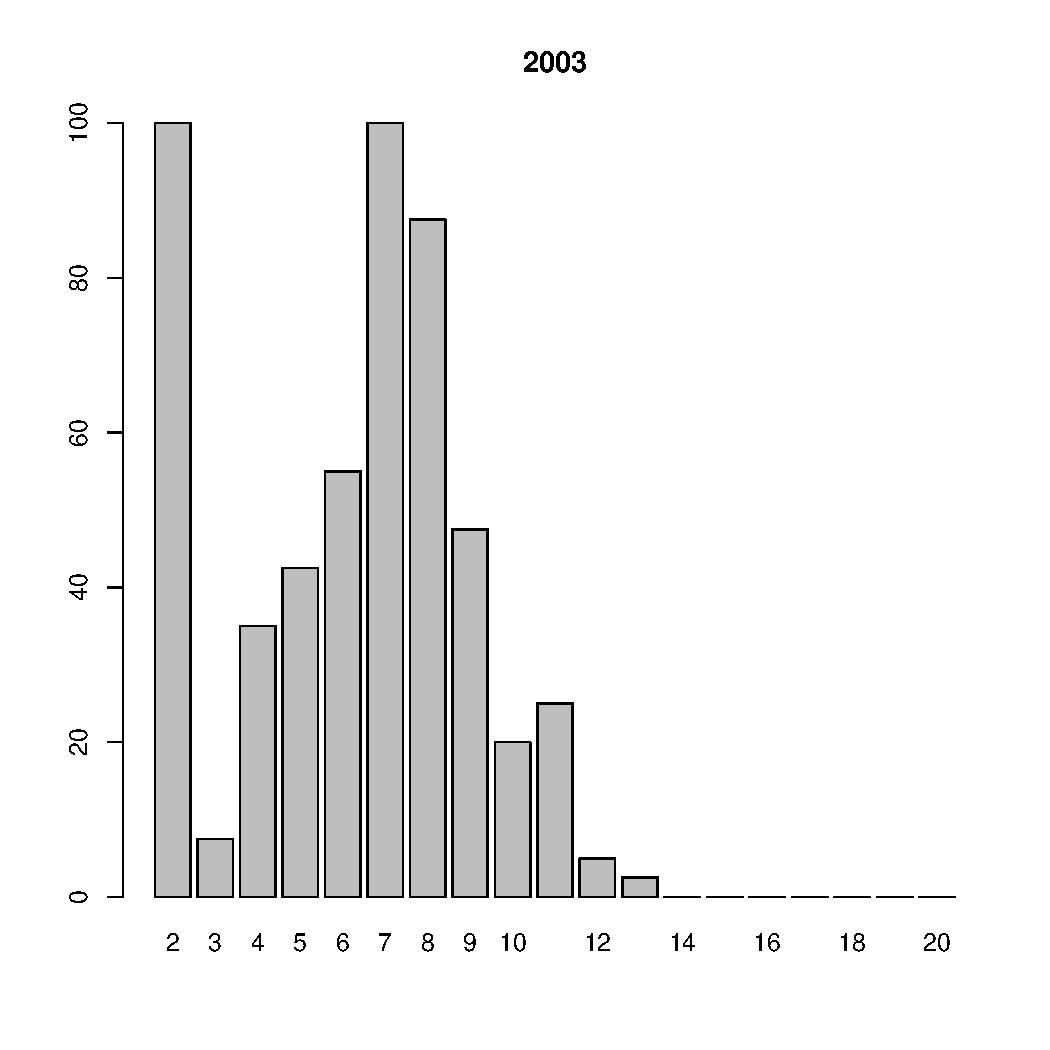
\includegraphics[width=60mm]{../White_Sea/Luvenga_Goreliy/high2_2003_.pdf}
	\end{center}
	\end{minipage}
	%
	\caption{Размерная структура {\it Macoma balthica} в ВГЛ о. Горелого}
	\label{ris:size_str_Goreliy_high}
	\end{figure}

%%%% вторая страница картинок с РС
	\begin{figure}[hp]

	\begin{minipage}[b]{.3\linewidth}
	\begin{center}
	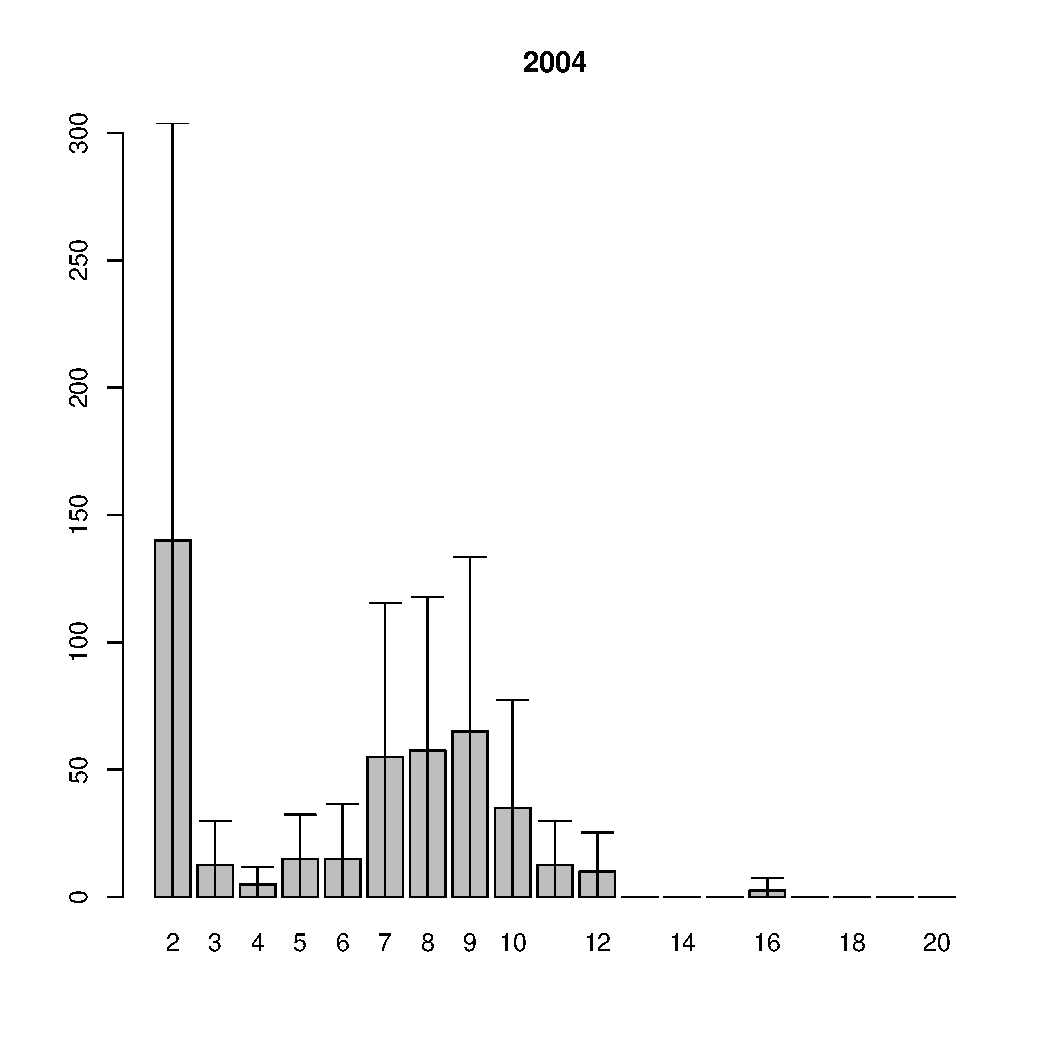
\includegraphics[width=60mm]{../White_Sea/Luvenga_Goreliy/high2_2004_.pdf}
	\end{center}
	\end{minipage}
	%
	\hfill
	%
	\begin{minipage}[b]{.3\linewidth}
	\begin{center}
	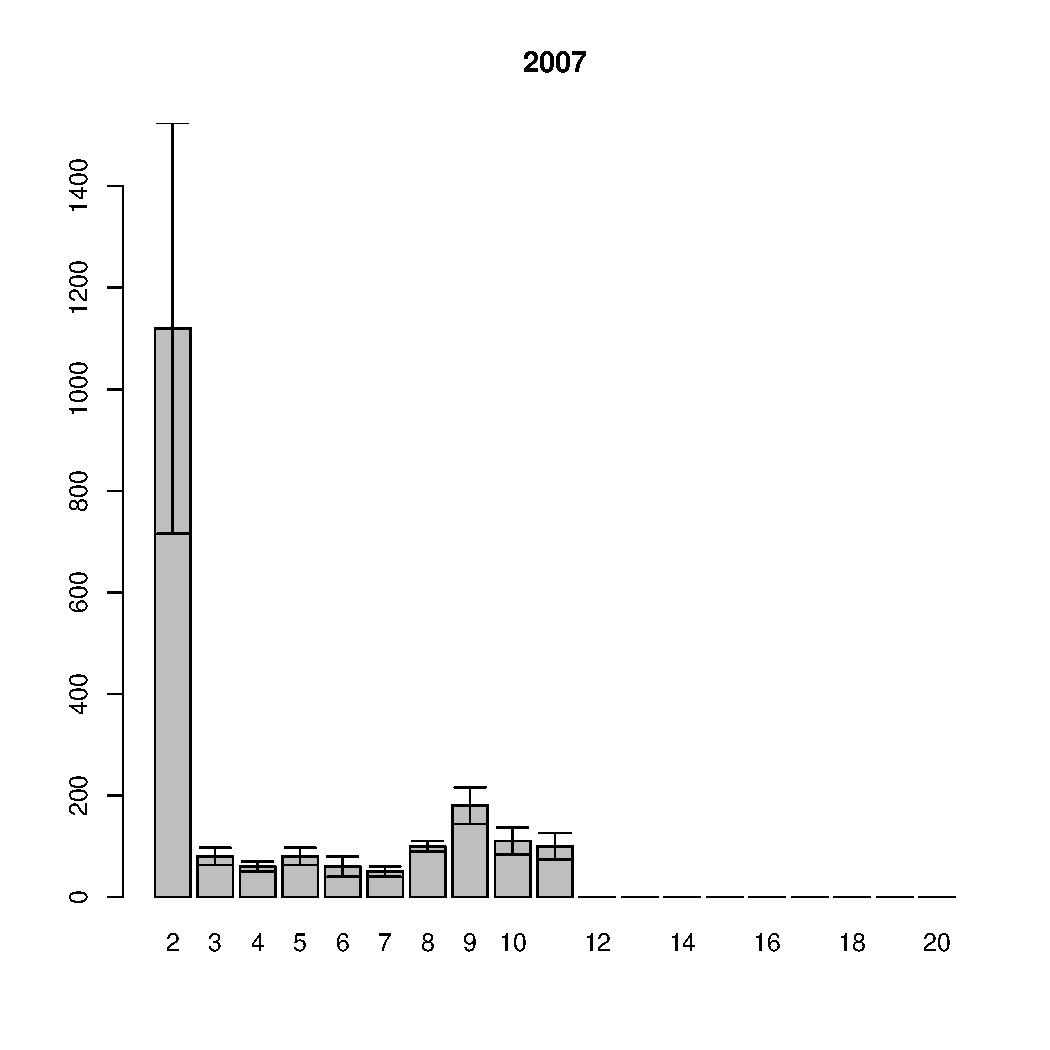
\includegraphics[width=60mm]{../White_Sea/Luvenga_Goreliy/high2_2007_.pdf}
	\end{center}
	\end{minipage}
	%
	\hfill
	%
	\begin{minipage}[b]{.3\linewidth}
	\begin{center}
	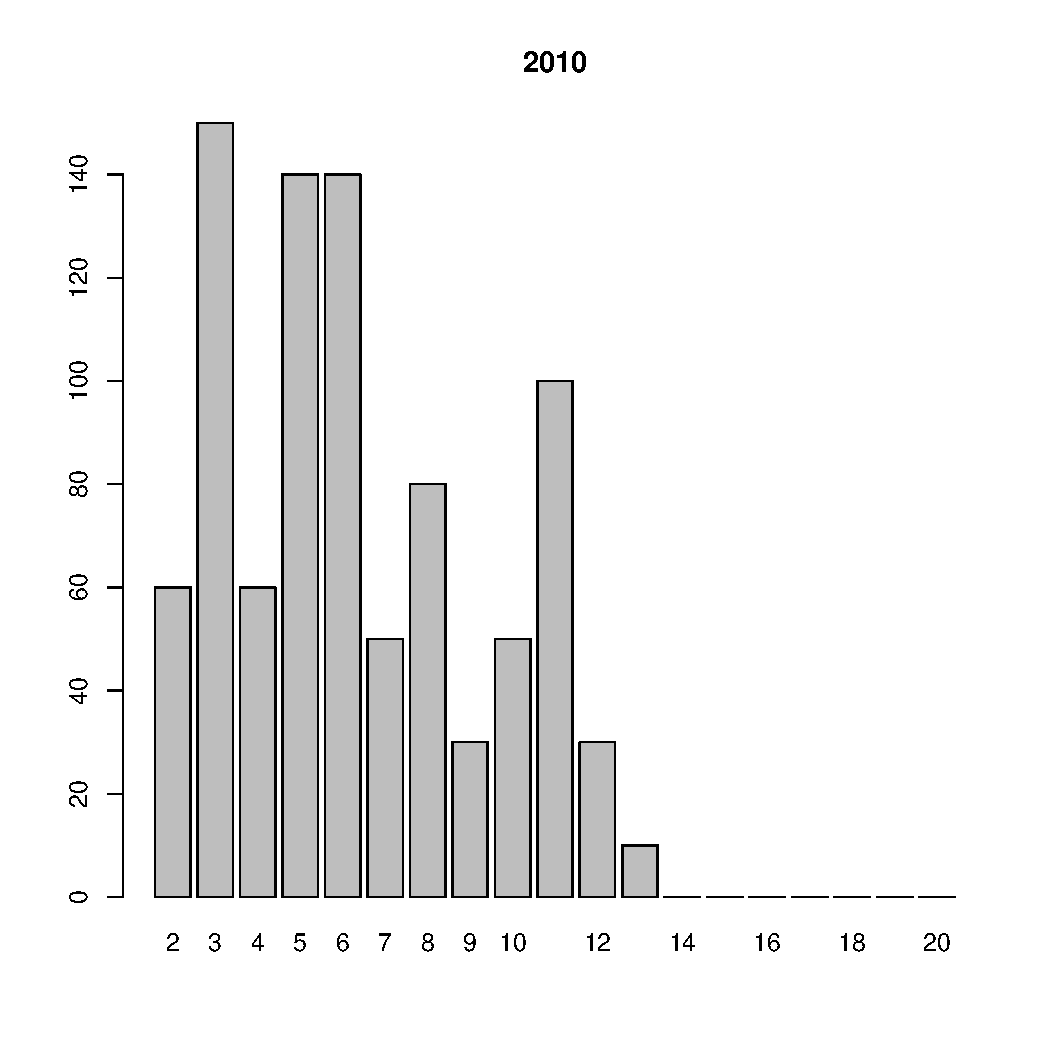
\includegraphics[width=60mm]{../White_Sea/Luvenga_Goreliy/high2_2010_.pdf}
	\end{center}
	\end{minipage}
	%
	%
	\begin{minipage}[b]{.3\linewidth}
	\begin{center}
	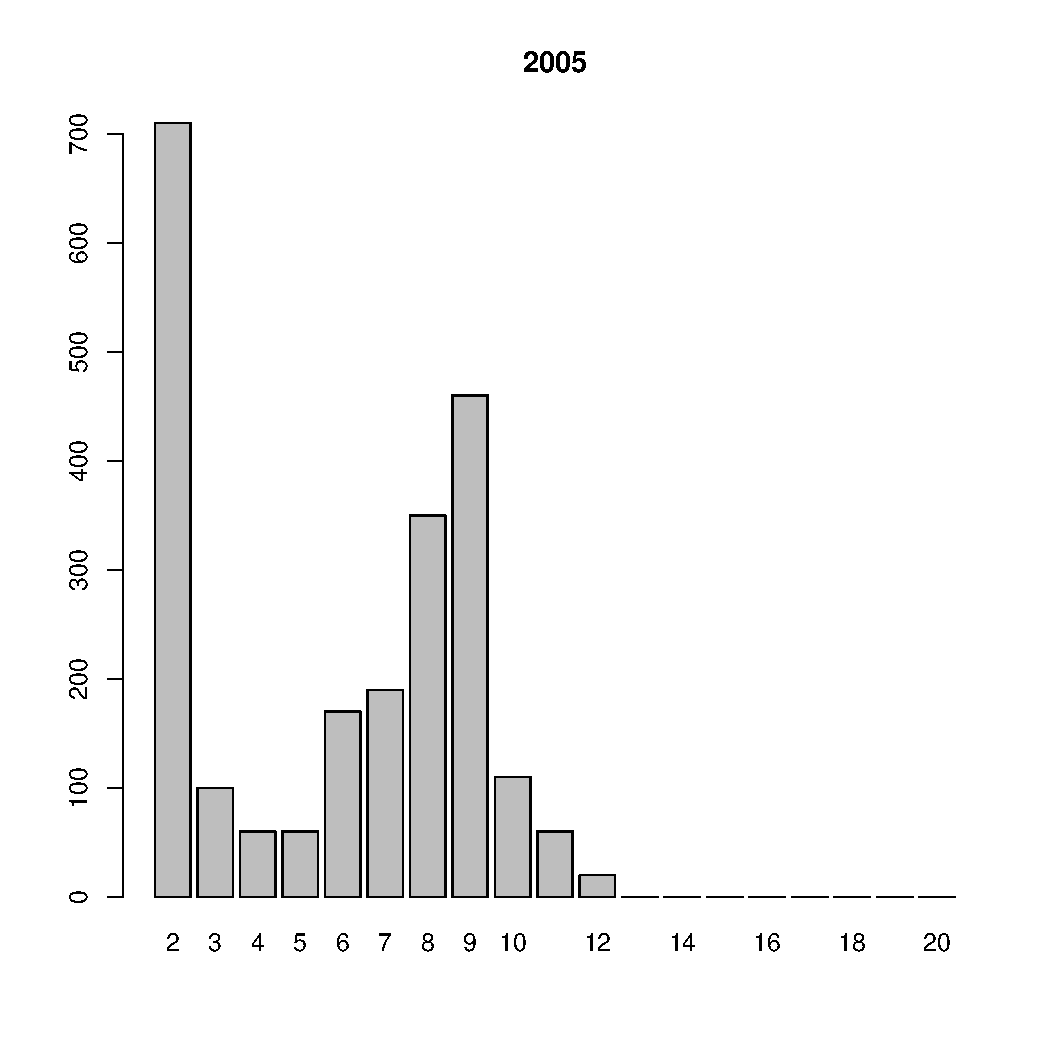
\includegraphics[width=60mm]{../White_Sea/Luvenga_Goreliy/high2_2005_.pdf}
	\end{center}
	\end{minipage}
	%
	\hfill	
	%
	\begin{minipage}[b]{.3\linewidth}
	\begin{center}
	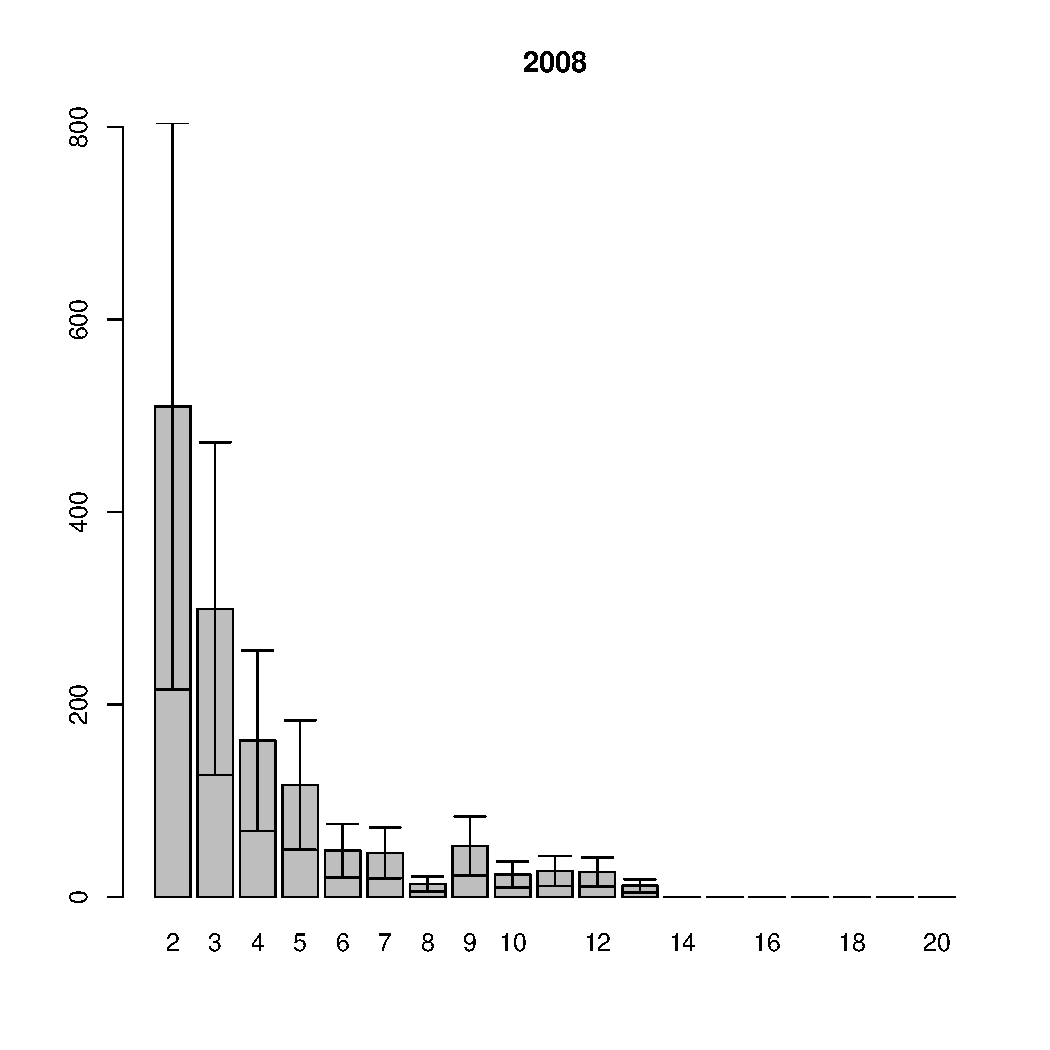
\includegraphics[width=60mm]{../White_Sea/Luvenga_Goreliy/high2_2008_.pdf}
	\end{center}
	\end{minipage}
	%
	\hfill
	%
	\begin{minipage}[b]{.3\linewidth}
	\begin{center}
	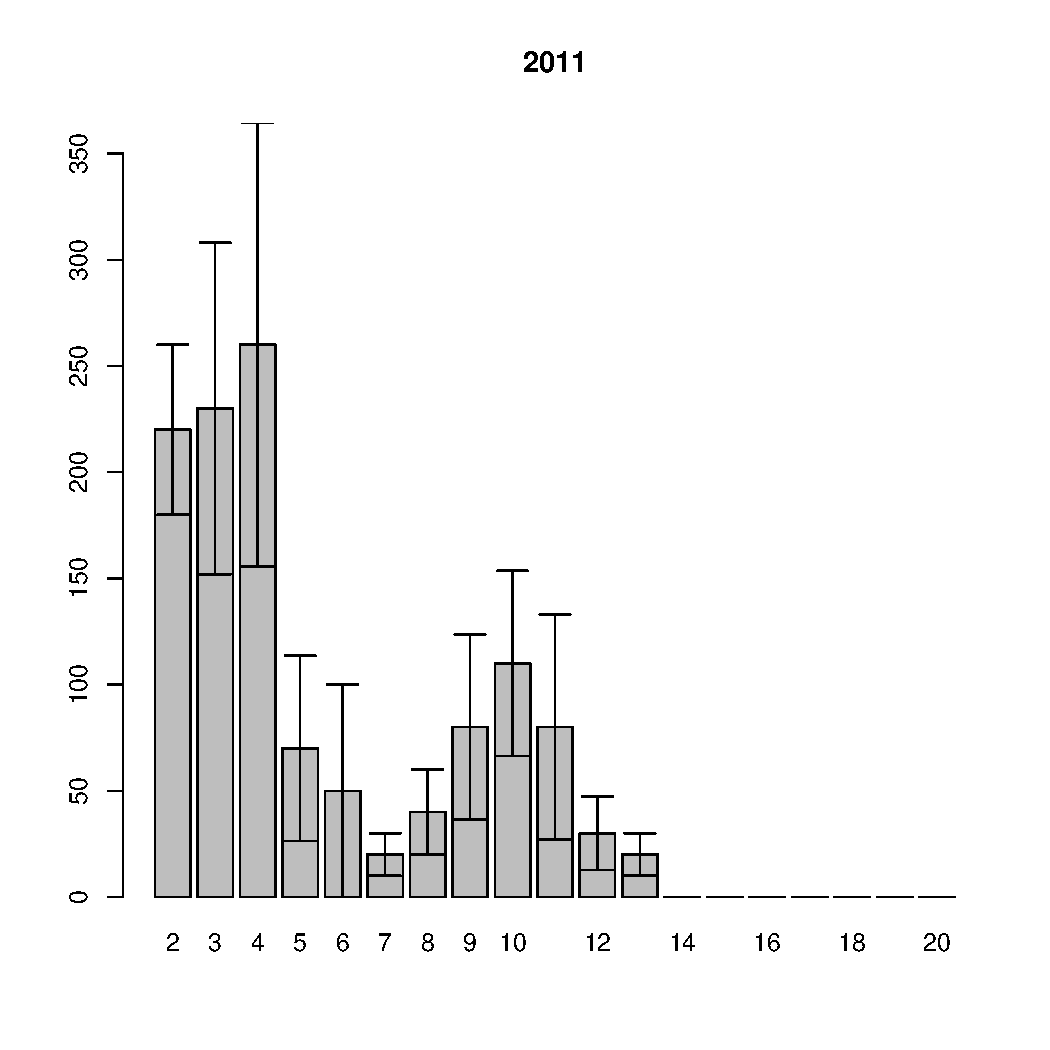
\includegraphics[width=60mm]{../White_Sea/Luvenga_Goreliy/high2_2011_.pdf}
	\end{center}
	\end{minipage}
	%
	%
	\begin{minipage}[b]{.3\linewidth}
	\begin{center}
	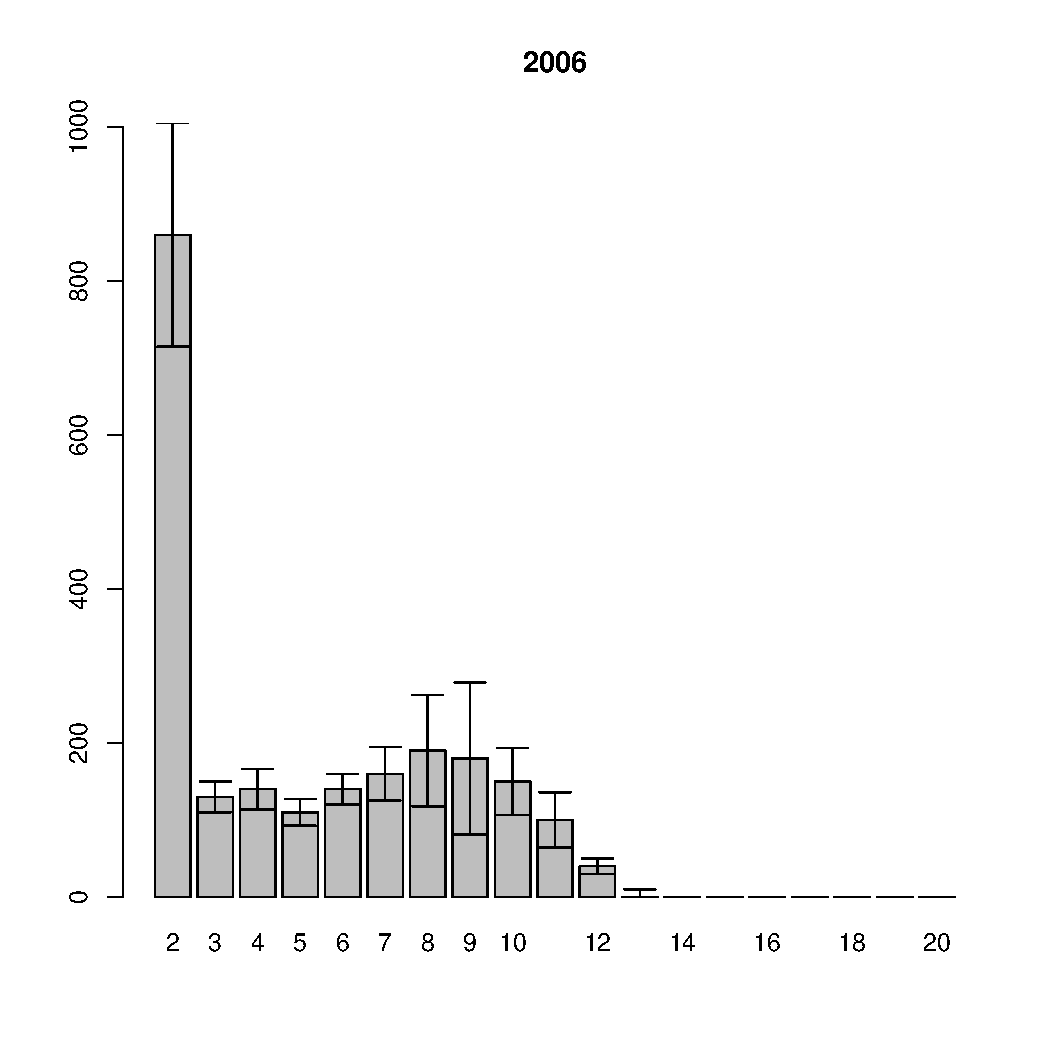
\includegraphics[width=60mm]{../White_Sea/Luvenga_Goreliy/high2_2006_.pdf}
	\end{center}
	\end{minipage}
	%
	\hfill
	%
	\begin{minipage}[b]{.3\linewidth}
	\begin{center}
	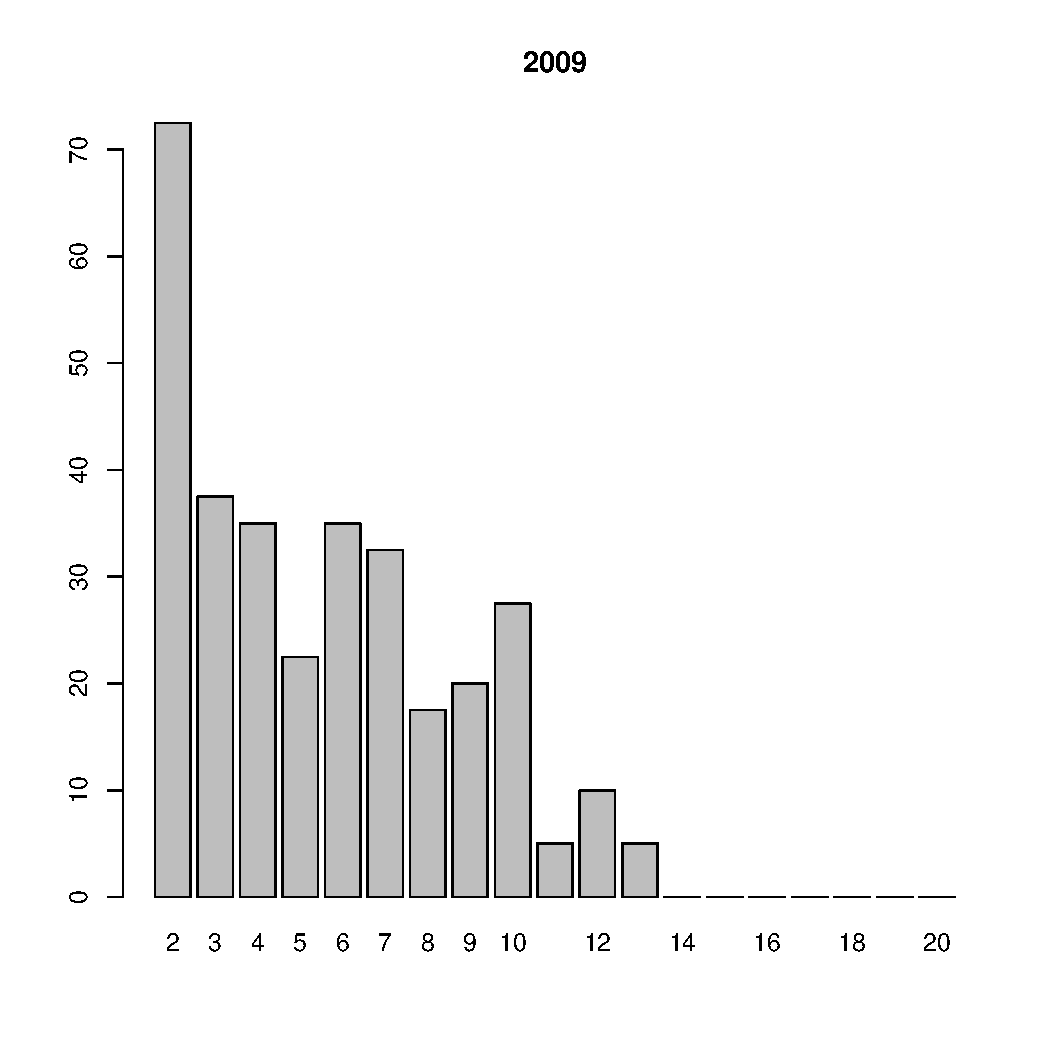
\includegraphics[width=60mm]{../White_Sea/Luvenga_Goreliy/high2_2009_.pdf}
	\end{center}
	\end{minipage}
	%
	\hfill
	%
	\begin{minipage}[b]{.3\linewidth}
	\begin{center}
	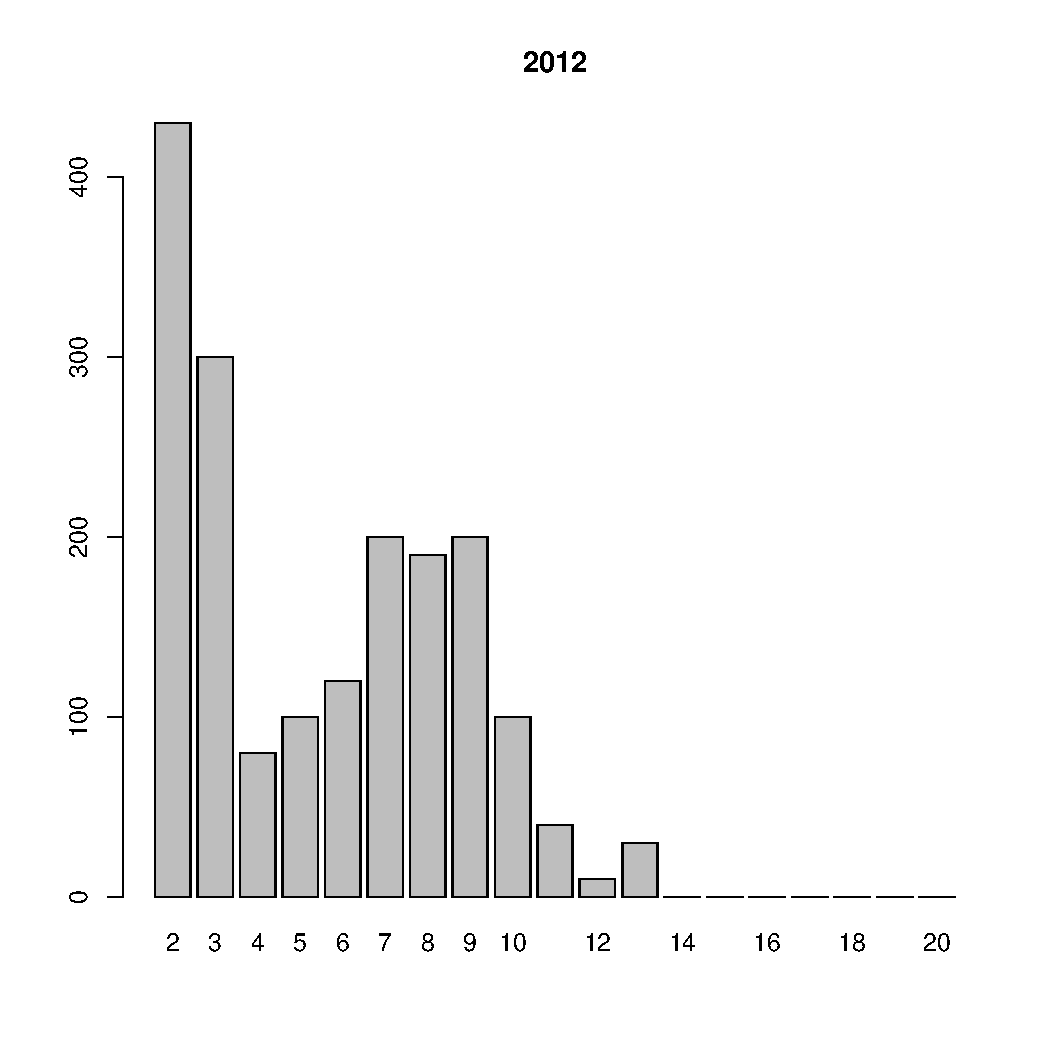
\includegraphics[width=60mm]{../White_Sea/Luvenga_Goreliy/high2_2012_.pdf}
	\end{center}
	\end{minipage}
	%
	\begin{center}
	Рис. \ref{ris:size_str_Goreliy_high} (продолжение). Размерная структура {\it Macoma balthica} в ВГЛ о. Горелого
	\end{center}
	\end{figure}


%%%%%%%%%%%%%%%%%%%%%%%%%%%%%%
%Горелый середина
	\begin{figure}[hp]

	\begin{minipage}[b]{.3\linewidth}
	\begin{center}
	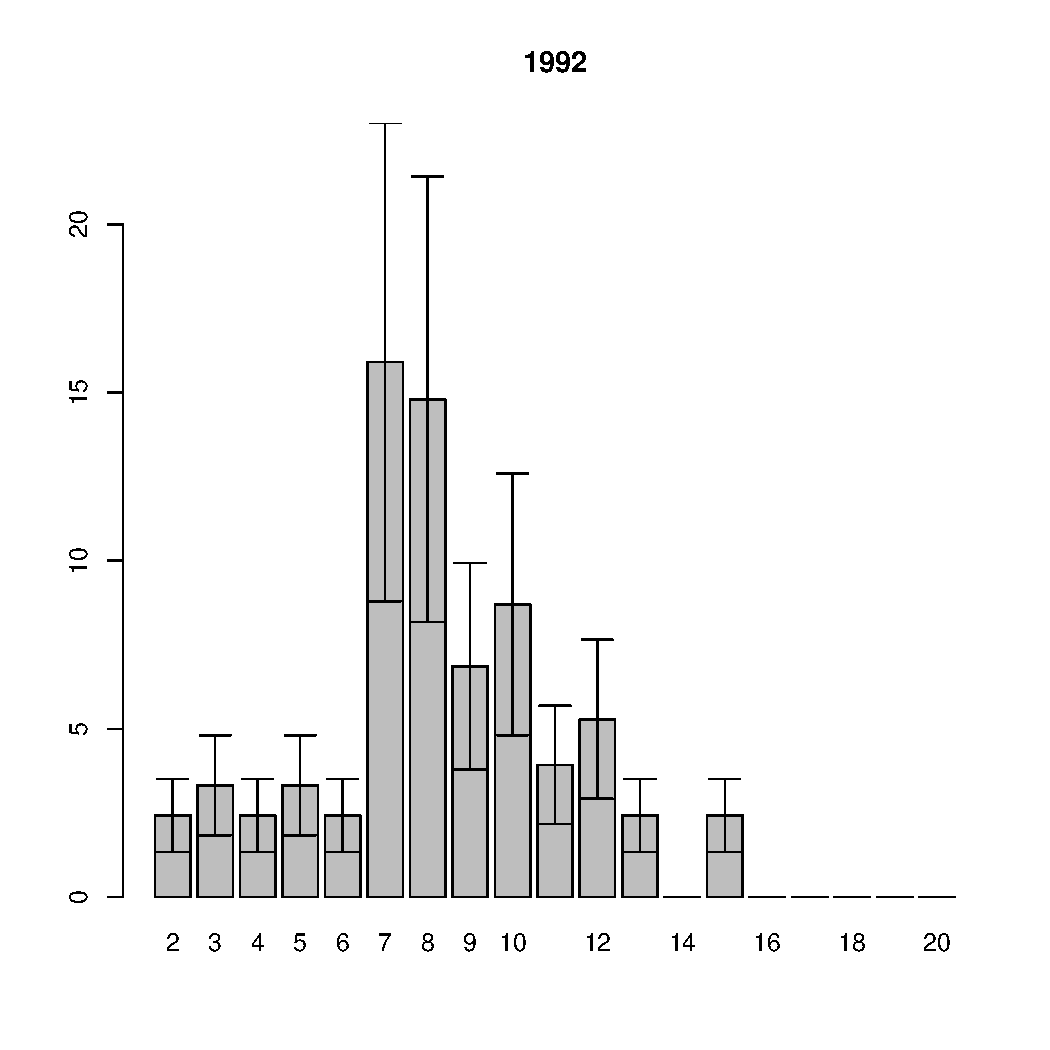
\includegraphics[width=60mm]{../White_Sea/Luvenga_Goreliy/middle2_1992_.pdf}	
	\end{center}
	\end{minipage}
	%
	\hfil %Это пружинка отодвигающая рисунки друг от друга
	%
	\begin{minipage}[b]{.3\linewidth}
	\begin{center}
	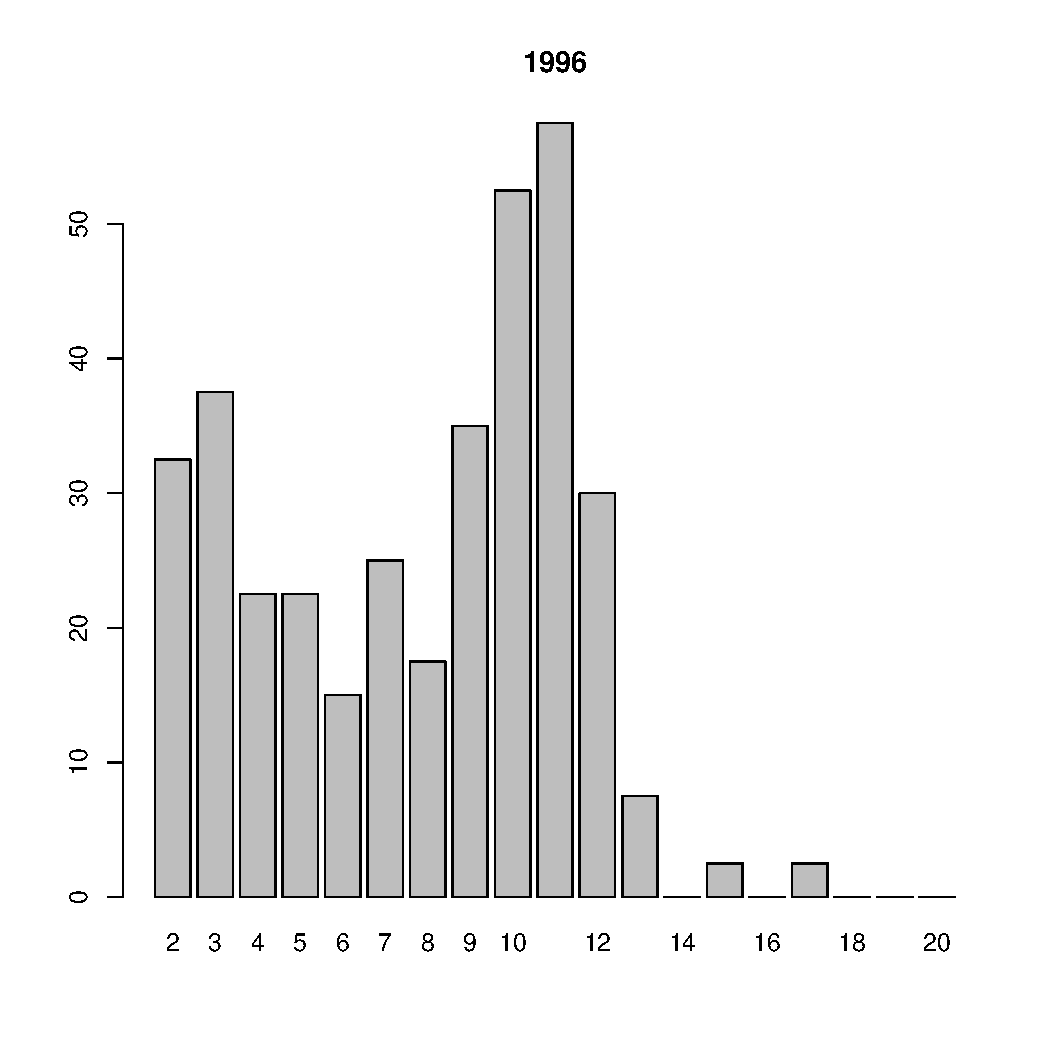
\includegraphics[width=60mm]{../White_Sea/Luvenga_Goreliy/middle2_1996_.pdf}
	\end{center}
	\end{minipage}
	%
	\hfil %Это пружинка отодвигающая рисунки друг от друга
	%
	\begin{minipage}[b]{.3\linewidth}
	\begin{center}
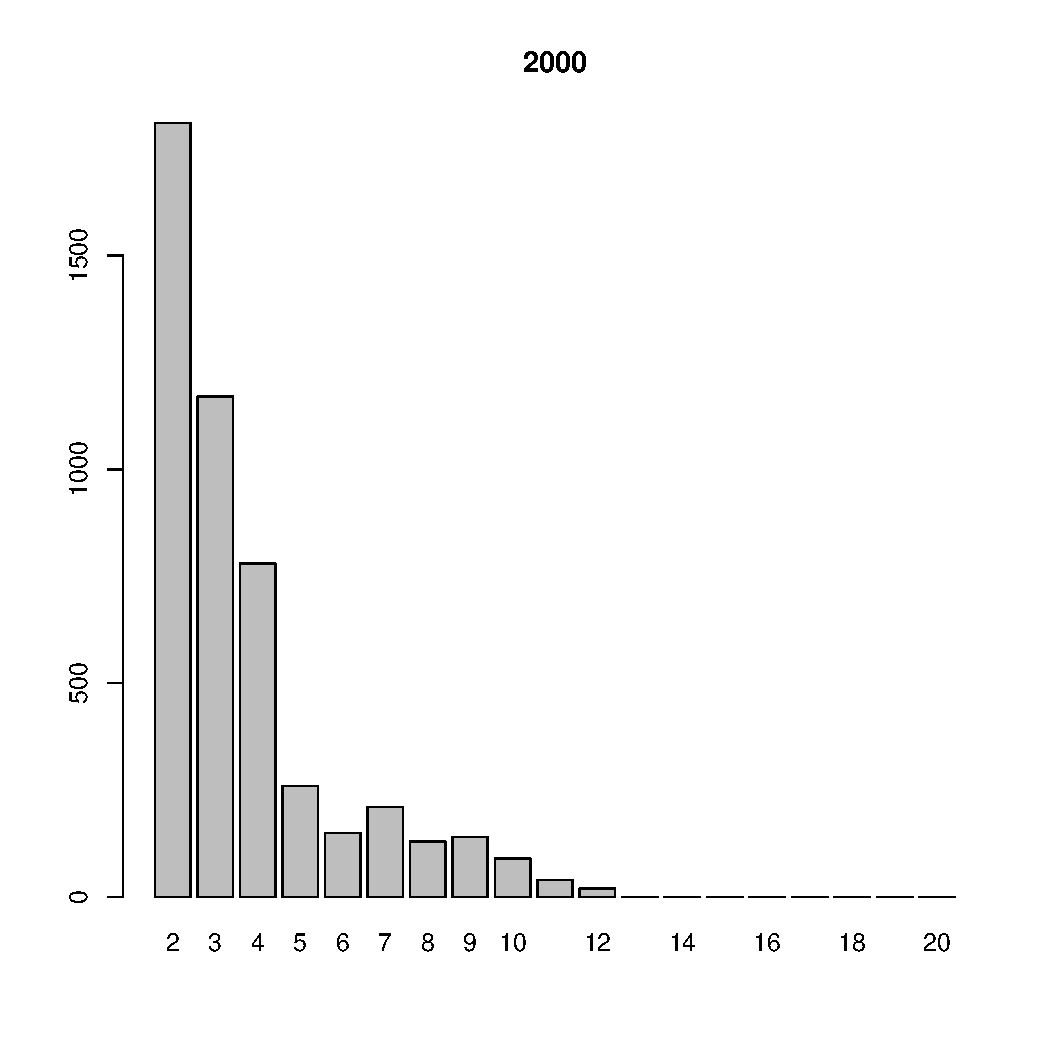
\includegraphics[width=60mm]{../White_Sea/Luvenga_Goreliy/middle2_2000_.pdf}
	\end{center}
	\end{minipage}
	%
	\begin{minipage}[b]{.3\linewidth}
	\begin{center}
	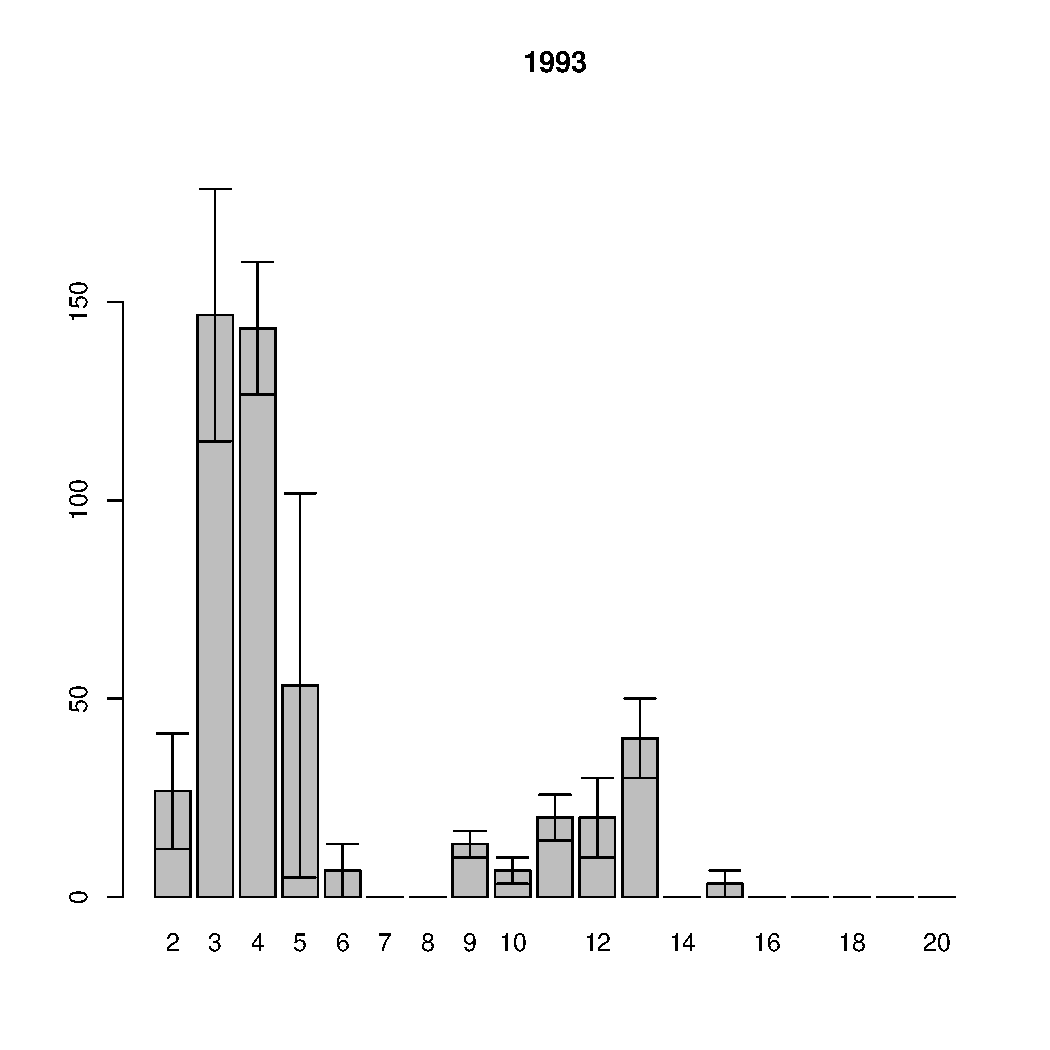
\includegraphics[width=60mm]{../White_Sea/Luvenga_Goreliy/middle2_1993_.pdf}
	\end{center}
	\end{minipage}
	%
	\hfil %Это пружинка отодвигающая рисунки друг от друга
	%
	\begin{minipage}[b]{.3\linewidth}
	\begin{center}
	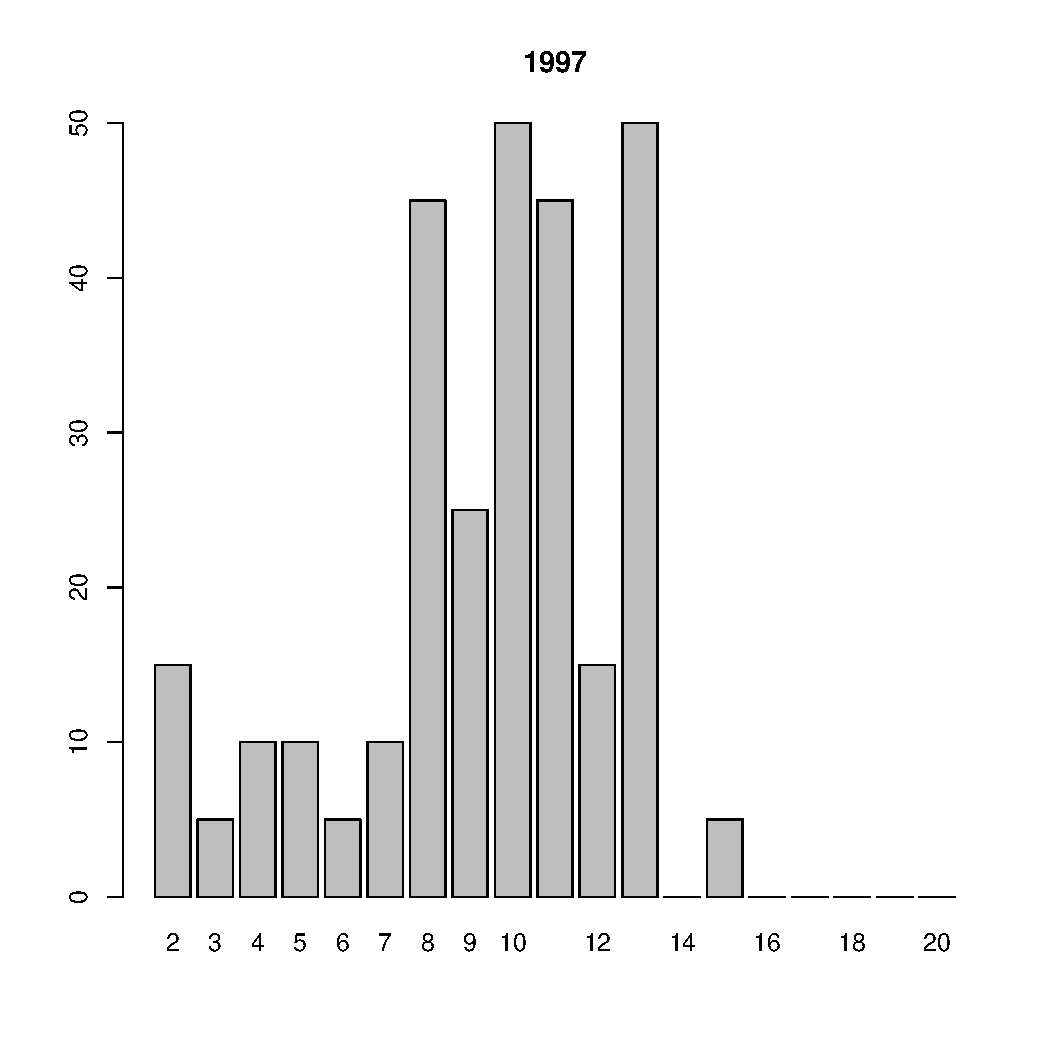
\includegraphics[width=60mm]{../White_Sea/Luvenga_Goreliy/middle2_1997_.pdf}
	\end{center}
	\end{minipage}
	%
	\hfil %Это пружинка отодвигающая рисунки друг от друга
	%
	\begin{minipage}[b]{.3\linewidth}
	\begin{center}
	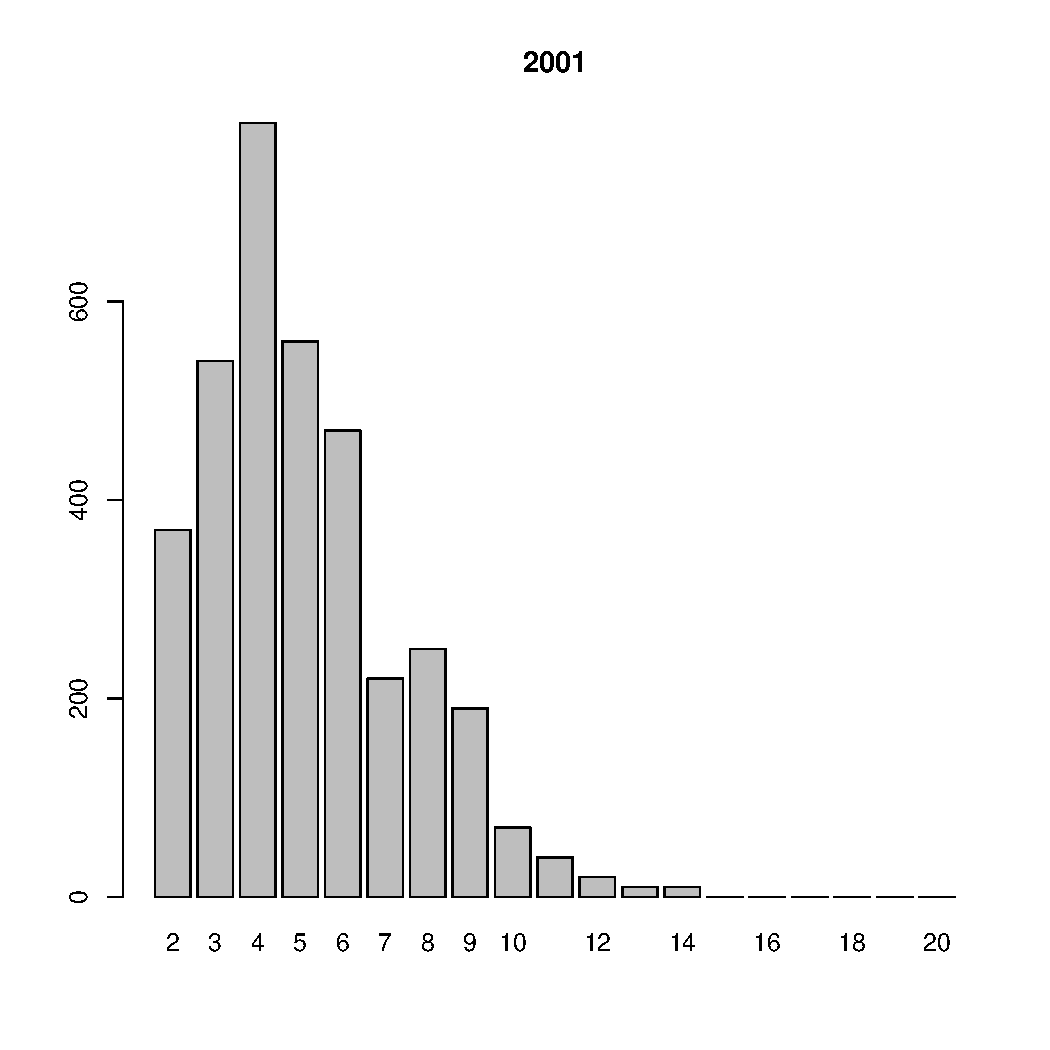
\includegraphics[width=60mm]{../White_Sea/Luvenga_Goreliy/middle2_2001_.pdf}
	\end{center}
	\end{minipage}
	%


	\begin{minipage}[b]{.3\linewidth}
	\begin{center}
	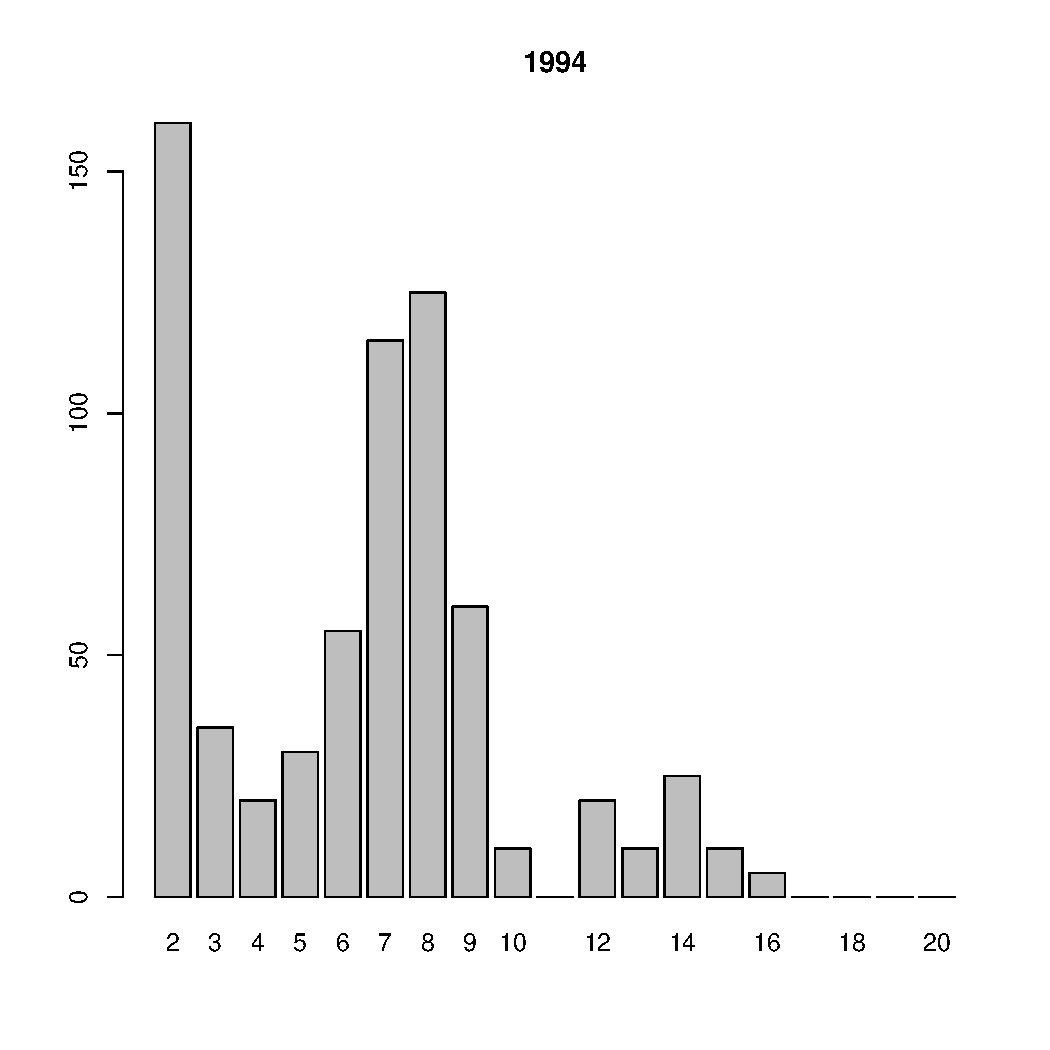
\includegraphics[width=60mm]{../White_Sea/Luvenga_Goreliy/middle2_1994_.pdf}
	\end{center}
	\end{minipage}
	%
	\hfill
	%
	\begin{minipage}[b]{.3\linewidth}
	\begin{center}
	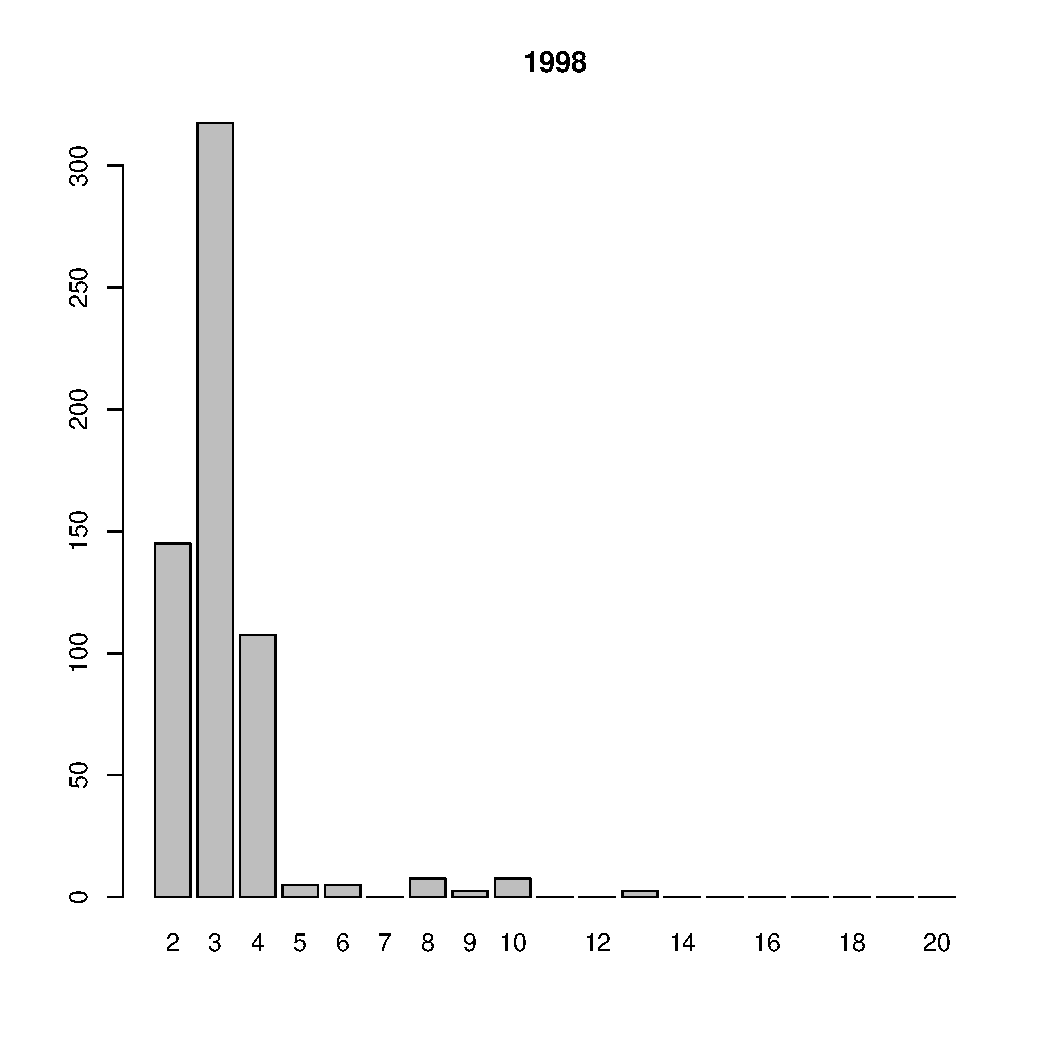
\includegraphics[width=60mm]{../White_Sea/Luvenga_Goreliy/middle2_1998_.pdf}
	\end{center}
	\end{minipage}	
	%
	\hfill
	%
	\begin{minipage}[b]{.3\linewidth}
	\begin{center}
	\includegraphics[width=60mm]{../White_Sea/Luvenga_Goreliy/middle2_2002_.pdf}
	\end{center}
	\end{minipage}
%\smallskip

	\begin{minipage}[b]{.3\linewidth}
	\begin{center}
	\includegraphics[width=60mm]{../White_Sea/Luvenga_Goreliy/middle2_1995_.pdf}
	\end{center}
	\end{minipage}
	%
	\hfill
	%
	\begin{minipage}[b]{.3\linewidth}
	\begin{center}
	\includegraphics[width=60mm]{../White_Sea/Luvenga_Goreliy/middle2_1999_.pdf}
	\end{center}
	\end{minipage}
	%
	\hfill
	%
	\begin{minipage}[b]{.3\linewidth}
	\begin{center}
	\includegraphics[width=60mm]{../White_Sea/Luvenga_Goreliy/middle2_2003_.pdf}
	\end{center}
	\end{minipage}
	%
\caption{Размерная структура {\it Macoma balthica} в СГЛ о. Горелого}
\label{ris:size_str_Goreliy_mid}
\end{figure}

%%%% вторая страница картинок с РС
	\begin{figure}[hp]

	\begin{minipage}[b]{.3\linewidth}
	\begin{center}
	\includegraphics[width=60mm]{../White_Sea/Luvenga_Goreliy/middle2_2004_.pdf}
	\end{center}
	\end{minipage}
	%
	\hfill
	%
	\begin{minipage}[b]{.3\linewidth}
	\begin{center}
	\includegraphics[width=60mm]{../White_Sea/Luvenga_Goreliy/middle2_2007_.pdf}
	\end{center}
	\end{minipage}
	%
	\hfill
	%
	\begin{minipage}[b]{.3\linewidth}
	\begin{center}
	\includegraphics[width=60mm]{../White_Sea/Luvenga_Goreliy/middle2_2010_.pdf}
	\end{center}
	\end{minipage}
	%
	%
	\begin{minipage}[b]{.3\linewidth}
	\begin{center}
	\includegraphics[width=60mm]{../White_Sea/Luvenga_Goreliy/middle2_2005_.pdf}
	\end{center}
	\end{minipage}
	%
	\hfill	
	%
	\begin{minipage}[b]{.3\linewidth}
	\begin{center}
	\includegraphics[width=60mm]{../White_Sea/Luvenga_Goreliy/middle2_2008_.pdf}
	\end{center}
	\end{minipage}
	%
	\hfill
	%
	\begin{minipage}[b]{.3\linewidth}
	\begin{center}
	\includegraphics[width=60mm]{../White_Sea/Luvenga_Goreliy/middle2_2011_.pdf}
	\end{center}
	\end{minipage}
	%
	%
	\begin{minipage}[b]{.3\linewidth}
	\begin{center}
	\includegraphics[width=60mm]{../White_Sea/Luvenga_Goreliy/middle2_2006_.pdf}
	\end{center}
	\end{minipage}
	%
	\hfill
	%
	\begin{minipage}[b]{.3\linewidth}
	\begin{center}
	\includegraphics[width=60mm]{../White_Sea/Luvenga_Goreliy/middle2_2009_.pdf}
	\end{center}
	\end{minipage}
	%
	\hfill
	%
	\begin{minipage}[b]{.3\linewidth}
	\begin{center}
	\includegraphics[width=60mm]{../White_Sea/Luvenga_Goreliy/middle2_2012_.pdf}
	\end{center}
	\end{minipage}
	%
	\begin{center}
Рис. \ref{ris:size_str_Goreliy_mid} (продолжение). Размерная структура {\it Macoma balthica} в СГЛ о. Горелого
\end{center}
\end{figure}

%%%%%%%%%%%%%%%%%%%%%%%%%%%%%%
%Горелый низ
	\begin{figure}[hp]

	\begin{minipage}[b]{.3\linewidth}
	\begin{center}
	\includegraphics[width=60mm]{../White_Sea/Luvenga_Goreliy/midlow2_1992_.pdf}	
	\end{center}
	\end{minipage}
	%
	\hfil %Это пружинка отодвигающая рисунки друг от друга
	%
	\begin{minipage}[b]{.3\linewidth}
	\begin{center}
	\includegraphics[width=60mm]{../White_Sea/Luvenga_Goreliy/midlow2_1996_.pdf}
	\end{center}
	\end{minipage}
	%
	\hfil %Это пружинка отодвигающая рисунки друг от друга
	%
	\begin{minipage}[b]{.3\linewidth}
	\begin{center}
\includegraphics[width=60mm]{../White_Sea/Luvenga_Goreliy/midlow2_2000_.pdf}
	\end{center}
	\end{minipage}
	%
	\begin{minipage}[b]{.3\linewidth}
	\begin{center}
	\includegraphics[width=60mm]{../White_Sea/Luvenga_Goreliy/midlow2_1993_.pdf}
	\end{center}
	\end{minipage}
	%
	\hfil %Это пружинка отодвигающая рисунки друг от друга
	%
	\begin{minipage}[b]{.3\linewidth}
	\begin{center}
	\includegraphics[width=60mm]{../White_Sea/Luvenga_Goreliy/midlow2_1997_.pdf}
	\end{center}
	\end{minipage}
	%
	\hfil %Это пружинка отодвигающая рисунки друг от друга
	%
	\begin{minipage}[b]{.3\linewidth}
	\begin{center}
	\includegraphics[width=60mm]{../White_Sea/Luvenga_Goreliy/midlow2_2001_.pdf}
	\end{center}
	\end{minipage}
	%


	\begin{minipage}[b]{.3\linewidth}
	\begin{center}
\includegraphics[width=60mm]{../White_Sea/Luvenga_Goreliy/midlow2_1994_.pdf}
	\end{center}
	\end{minipage}
	%
	\hfill
	%
	\begin{minipage}[b]{.3\linewidth}
	\begin{center}
	\includegraphics[width=60mm]{../White_Sea/Luvenga_Goreliy/midlow2_1998_.pdf}
	\end{center}
	\end{minipage}	
	%
	\hfill
	%
	\begin{minipage}[b]{.3\linewidth}
	\begin{center}
	\includegraphics[width=60mm]{../White_Sea/Luvenga_Goreliy/midlow2_2002_.pdf}
	\end{center}
	\end{minipage}
%\smallskip

	\begin{minipage}[b]{.3\linewidth}
	\begin{center}
	\includegraphics[width=60mm]{../White_Sea/Luvenga_Goreliy/midlow2_1995_.pdf}
	\end{center}
	\end{minipage}
	%
	\hfill
	%
	\begin{minipage}[b]{.3\linewidth}
	\begin{center}
	\includegraphics[width=60mm]{../White_Sea/Luvenga_Goreliy/midlow2_1999_.pdf}
	\end{center}
	\end{minipage}
	%
	\hfill
	%
	\begin{minipage}[b]{.3\linewidth}
	\begin{center}
	\includegraphics[width=60mm]{../White_Sea/Luvenga_Goreliy/midlow2_2003_.pdf}
	\end{center}
	\end{minipage}
	%
\caption{Размерная структура {\it Macoma balthica} в НГЛ о. Горелого}
\label{ris:size_str_Goreliy_midlow}
\end{figure}

%%%% вторая страница картинок с РС
	\begin{figure}[hp]

	\begin{minipage}[b]{.3\linewidth}
	\begin{center}
	\includegraphics[width=60mm]{../White_Sea/Luvenga_Goreliy/midlow2_2004_.pdf}
	\end{center}
	\end{minipage}
	%
	\hfill
	%
	\begin{minipage}[b]{.3\linewidth}
	\begin{center}
	\includegraphics[width=60mm]{../White_Sea/Luvenga_Goreliy/midlow2_2007_.pdf}
	\end{center}
	\end{minipage}
	%
	\hfill
	%
	\begin{minipage}[b]{.3\linewidth}
	\begin{center}
	\includegraphics[width=60mm]{../White_Sea/Luvenga_Goreliy/midlow2_2010_.pdf}
	\end{center}
	\end{minipage}
	%
	%
	\begin{minipage}[b]{.3\linewidth}
	\begin{center}
	\includegraphics[width=60mm]{../White_Sea/Luvenga_Goreliy/midlow2_2005_.pdf}
	\end{center}
	\end{minipage}
	%
	\hfill	
	%
	\begin{minipage}[b]{.3\linewidth}
	\begin{center}
	\includegraphics[width=60mm]{../White_Sea/Luvenga_Goreliy/midlow2_2008_.pdf}
	\end{center}
	\end{minipage}
	%
	\hfill
	%
	\begin{minipage}[b]{.3\linewidth}
	\begin{center}
	\includegraphics[width=60mm]{../White_Sea/Luvenga_Goreliy/midlow2_2011_.pdf}
	\end{center}
	\end{minipage}
	%
	%
	\begin{minipage}[b]{.3\linewidth}
	\begin{center}
	\includegraphics[width=60mm]{../White_Sea/Luvenga_Goreliy/midlow2_2006_.pdf}
	\end{center}
	\end{minipage}
	%
	\hfill
	%
	\begin{minipage}[b]{.3\linewidth}
	\begin{center}
	\includegraphics[width=60mm]{../White_Sea/Luvenga_Goreliy/midlow2_2009_.pdf}
	\end{center}
	\end{minipage}
	%
	\hfill
	%
	\begin{minipage}[b]{.3\linewidth}
	\begin{center}
	\includegraphics[width=60mm]{../White_Sea/Luvenga_Goreliy/midlow2_2012_.pdf}
	\end{center}
	\end{minipage}
	%
\begin{center}
Рис. \ref{ris:size_str_Goreliy_midlow} (продолжение). Размерная структура {\it Macoma balthica} в НГЛ о. Горелого
\end{center}
\end{figure}




%%%%%%%%%%%%%%%%%%%%%%%%%%%%%%
%Горелый ноль глубин
	\begin{figure}[hp]

	\begin{minipage}[b]{.3\linewidth}
	\begin{center}
	\includegraphics[width=60mm]{../White_Sea/Luvenga_Goreliy/low2_1992_.pdf}	
	\end{center}
	\end{minipage}
	%
	\hfil %Это пружинка отодвигающая рисунки друг от друга
	%
	\begin{minipage}[b]{.3\linewidth}
	\begin{center}
	\includegraphics[width=60mm]{../White_Sea/Luvenga_Goreliy/low2_1996_.pdf}
	\end{center}
	\end{minipage}
	%
	\hfil %Это пружинка отодвигающая рисунки друг от друга
	%
	\begin{minipage}[b]{.3\linewidth}
	\begin{center}
\includegraphics[width=60mm]{../White_Sea/Luvenga_Goreliy/low2_2000_.pdf}
	\end{center}
	\end{minipage}
	%
	\begin{minipage}[b]{.3\linewidth}
	\begin{center}
	\includegraphics[width=60mm]{../White_Sea/Luvenga_Goreliy/low2_1993_.pdf}
	\end{center}
	\end{minipage}
	%
	\hfil %Это пружинка отодвигающая рисунки друг от друга
	%
	\begin{minipage}[b]{.3\linewidth}
	\begin{center}
	\includegraphics[width=60mm]{../White_Sea/Luvenga_Goreliy/low2_1997_.pdf}
	\end{center}
	\end{minipage}
	%
	\hfil %Это пружинка отодвигающая рисунки друг от друга
	%
	\begin{minipage}[b]{.3\linewidth}
	\begin{center}
	\includegraphics[width=60mm]{../White_Sea/Luvenga_Goreliy/low2_2001_.pdf}
	\end{center}
	\end{minipage}
	%


	\begin{minipage}[b]{.3\linewidth}
	\begin{center}
	\includegraphics[width=60mm]{../White_Sea/Luvenga_Goreliy/low2_1994_.pdf}
	\end{center}
	\end{minipage}
	%
	\hfill
	%
	\begin{minipage}[b]{.3\linewidth}
	\begin{center}
	\includegraphics[width=60mm]{../White_Sea/Luvenga_Goreliy/low2_1998_.pdf}
	\end{center}
	\end{minipage}	
	%
	\hfill
	%
	\begin{minipage}[b]{.3\linewidth}
	\begin{center}
	\includegraphics[width=60mm]{../White_Sea/Luvenga_Goreliy/low2_2002_.pdf}
	\end{center}
	\end{minipage}
%\smallskip

	\begin{minipage}[b]{.3\linewidth}
	\begin{center}
	\includegraphics[width=60mm]{../White_Sea/Luvenga_Goreliy/low2_1995_.pdf}
	\end{center}
	\end{minipage}
	%
	\hfill
	%
	\begin{minipage}[b]{.3\linewidth}
	\begin{center}
	\includegraphics[width=60mm]{../White_Sea/Luvenga_Goreliy/low2_1999_.pdf}
	\end{center}
	\end{minipage}
	%
	\hfill
	%
	\begin{minipage}[b]{.3\linewidth}
	\begin{center}
	\includegraphics[width=60mm]{../White_Sea/Luvenga_Goreliy/low2_2003_.pdf}
	\end{center}
	\end{minipage}
	%
\caption{Размерная структура {\it Macoma balthica} в районе нуля глубин о. Горелого}
\label{ris:size_str_Goreliy_low}
\end{figure}

%%%% вторая страница картинок с РС
	\begin{figure}[hp]

	\begin{minipage}[b]{.3\linewidth}
	\begin{center}
	\includegraphics[width=60mm]{../White_Sea/Luvenga_Goreliy/low2_2004_.pdf}
	\end{center}
	\end{minipage}
	%
	\hfill
	%
	\begin{minipage}[b]{.3\linewidth}
	\begin{center}
	\includegraphics[width=60mm]{../White_Sea/Luvenga_Goreliy/low2_2007_.pdf}
	\end{center}
	\end{minipage}
	%
	\hfill
	%
	\begin{minipage}[b]{.3\linewidth}
	\begin{center}
	\includegraphics[width=60mm]{../White_Sea/Luvenga_Goreliy/low2_2010_.pdf}
	\end{center}
	\end{minipage}
	%
	%
	\begin{minipage}[b]{.3\linewidth}
	\begin{center}
	\includegraphics[width=60mm]{../White_Sea/Luvenga_Goreliy/low2_2005_.pdf}
	\end{center}
	\end{minipage}
	%
	\hfill	
	%
	\begin{minipage}[b]{.3\linewidth}
	\begin{center}
	\includegraphics[width=60mm]{../White_Sea/Luvenga_Goreliy/low2_2008_.pdf}
	\end{center}
	\end{minipage}
	%
	\hfill
	%
	\begin{minipage}[b]{.3\linewidth}
	\begin{center}
	\includegraphics[width=60mm]{../White_Sea/Luvenga_Goreliy/low2_2011_.pdf}
	\end{center}
	\end{minipage}
	%
	%
	\begin{minipage}[b]{.3\linewidth}
	\begin{center}
	\includegraphics[width=60mm]{../White_Sea/Luvenga_Goreliy/low2_2006_.pdf}
	\end{center}
	\end{minipage}
	%
	\hfill
	%
	\begin{minipage}[b]{.3\linewidth}
	\begin{center}
	\includegraphics[width=60mm]{../White_Sea/Luvenga_Goreliy/low2_2009_.pdf}
	\end{center}
	\end{minipage}
	%
	\hfill
	%
	\begin{minipage}[b]{.3\linewidth}
	\begin{center}
	\includegraphics[width=60mm]{../White_Sea/Luvenga_Goreliy/low2_2012_.pdf}
	\end{center}
	\end{minipage}
	%
\begin{center}
Рис. \ref{ris:size_str_Goreliy_low} (продолжение). Размерная структура {\it Macoma balthica} у нуля глубин  о. Горелого
\end{center}
\end{figure}



%%%%%%%%%%%%%%%%%%%%%%%%%%%%%%
%2 разрез верхний пляж
	\begin{figure}[hp]

	\begin{minipage}[b]{.3\linewidth}
	\begin{center}
	\includegraphics[width=60mm]{../White_Sea/Luvenga_II_razrez/high_beatch2_1992_.pdf}	
	\end{center}
	\end{minipage}
	%
	\hfil %Это пружинка отодвигающая рисунки друг от друга
	%
	\begin{minipage}[b]{.3\linewidth}
	\begin{center}
	\includegraphics[width=60mm]{../White_Sea/Luvenga_II_razrez/high_beatch2_1996_.pdf}
	\end{center}
	\end{minipage}
	%
	\hfil %Это пружинка отодвигающая рисунки друг от друга
	%
	\begin{minipage}[b]{.3\linewidth}
	\begin{center}
\includegraphics[width=60mm]{../White_Sea/Luvenga_II_razrez/high_beatch2_2000_.pdf}
	\end{center}
	\end{minipage}
	%
	\begin{minipage}[b]{.3\linewidth}
	\begin{center}
	\includegraphics[width=60mm]{../White_Sea/Luvenga_II_razrez/high_beatch2_1993_.pdf}
	\end{center}
	\end{minipage}
	%
	\hfil %Это пружинка отодвигающая рисунки друг от друга
	%
	\begin{minipage}[b]{.3\linewidth}
	\begin{center}
	\includegraphics[width=60mm]{../White_Sea/Luvenga_II_razrez/high_beatch2_1997_.pdf}
	\end{center}
	\end{minipage}
	%
	\hfil %Это пружинка отодвигающая рисунки друг от друга
	%
	\begin{minipage}[b]{.3\linewidth}
	\begin{center}
	\includegraphics[width=60mm]{../White_Sea/Luvenga_II_razrez/high_beatch2_2002_.pdf}
	\end{center}
	\end{minipage}
	%


	\begin{minipage}[b]{.3\linewidth}
	\begin{center}
	\includegraphics[width=60mm]{../White_Sea/Luvenga_II_razrez/high_beatch2_1994_.pdf}
	\end{center}
	\end{minipage}
	%
	\hfill
	%
	\begin{minipage}[b]{.3\linewidth}
	\begin{center}
	\includegraphics[width=60mm]{../White_Sea/Luvenga_II_razrez/high_beatch2_1998_.pdf}
	\end{center}
	\end{minipage}	
	%
	\hfill
	%
	\begin{minipage}[b]{.3\linewidth}
	\begin{center}
	\includegraphics[width=60mm]{../White_Sea/Luvenga_II_razrez/high_beatch2_2004_.pdf}
	\end{center}
	\end{minipage}
%\smallskip

	\begin{minipage}[b]{.3\linewidth}
	\begin{center}
	\includegraphics[width=60mm]{../White_Sea/Luvenga_II_razrez/high_beatch2_1995_.pdf}
	\end{center}
	\end{minipage}
	%
	\hfill
	%
	\begin{minipage}[b]{.3\linewidth}
	\begin{center}
	\includegraphics[width=60mm]{../White_Sea/Luvenga_II_razrez/high_beatch2_1999_.pdf}
	\end{center}
	\end{minipage}
	%
	\hfill
	%
	\begin{minipage}[b]{.3\linewidth}
	\begin{center}

	\end{center}
	\end{minipage}
	%
\caption{Размерная структура {\it Macoma balthica} на верхнем пляже материковой литорали в районе пос.~ Лувеньга}
\label{ris:size_str_2razrez_high}
\end{figure}


%%%%%%%%%%%%%%%%%%%%%%%%%%%%%%
%2 разрез фукоиды
	\begin{figure}[hp]

	\begin{minipage}[b]{.3\linewidth}
	\begin{center}
	\includegraphics[width=60mm]{../White_Sea/Luvenga_II_razrez/fucus_zone2_1992_.pdf}	
	\end{center}
	\end{minipage}
	%
	\hfil %Это пружинка отодвигающая рисунки друг от друга
	%
	\begin{minipage}[b]{.3\linewidth}
	\begin{center}
	\includegraphics[width=60mm]{../White_Sea/Luvenga_II_razrez/fucus_zone2_1996_.pdf}
	\end{center}
	\end{minipage}
	%
	\hfil %Это пружинка отодвигающая рисунки друг от друга
	%
	\begin{minipage}[b]{.3\linewidth}
	\begin{center}
\includegraphics[width=60mm]{../White_Sea/Luvenga_II_razrez/fucus_zone2_2000_.pdf}
	\end{center}
	\end{minipage}
	%
	\begin{minipage}[b]{.3\linewidth}
	\begin{center}
	\includegraphics[width=60mm]{../White_Sea/Luvenga_II_razrez/fucus_zone2_1993_.pdf}
	\end{center}
	\end{minipage}
	%
	\hfil %Это пружинка отодвигающая рисунки друг от друга
	%
	\begin{minipage}[b]{.3\linewidth}
	\begin{center}
	\includegraphics[width=60mm]{../White_Sea/Luvenga_II_razrez/fucus_zone2_1997_.pdf}
	\end{center}
	\end{minipage}
	%
	\hfil %Это пружинка отодвигающая рисунки друг от друга
	%
	\begin{minipage}[b]{.3\linewidth}
	\begin{center}
	\includegraphics[width=60mm]{../White_Sea/Luvenga_II_razrez/fucus_zone2_2002_.pdf}
	\end{center}
	\end{minipage}
	%


	\begin{minipage}[b]{.3\linewidth}
	\begin{center}
	\includegraphics[width=60mm]{../White_Sea/Luvenga_II_razrez/fucus_zone2_1994_.pdf}
	\end{center}
	\end{minipage}
	%
	\hfill
	%
	\begin{minipage}[b]{.3\linewidth}
	\begin{center}
	\includegraphics[width=60mm]{../White_Sea/Luvenga_II_razrez/fucus_zone2_1998_.pdf}
	\end{center}
	\end{minipage}	
	%
	\hfill
	%
	\begin{minipage}[b]{.3\linewidth}
	\begin{center}
	\includegraphics[width=60mm]{../White_Sea/Luvenga_II_razrez/fucus_zone2_2004_.pdf}
	\end{center}
	\end{minipage}
%\smallskip

	\begin{minipage}[b]{.3\linewidth}
	\begin{center}
	\includegraphics[width=60mm]{../White_Sea/Luvenga_II_razrez/fucus_zone2_1995_.pdf}
	\end{center}
	\end{minipage}
	%
	\hfill
	%
	\begin{minipage}[b]{.3\linewidth}
	\begin{center}
	\includegraphics[width=60mm]{../White_Sea/Luvenga_II_razrez/fucus_zone2_1999_.pdf}
	\end{center}
	\end{minipage}
	%
	\hfill
	%
	\begin{minipage}[b]{.3\linewidth}
	\begin{center}

	\end{center}
	\end{minipage}
	%
\caption{Размерная структура {\it Macoma balthica} в поясе фукоидов материковой литорали в районе пос. Лувеньга}
\label{ris:size_str_2razrez_fucus}
\end{figure}


%%%%%%%%%%%%%%%%%%%%%%%%%%%%%%
%2 разрез зостера
	\begin{figure}[hp]

	\begin{minipage}[b]{.3\linewidth}
	\begin{center}
	\includegraphics[width=60mm]{../White_Sea/Luvenga_II_razrez/zostera_zone2_1992_.pdf}	
	\end{center}
	\end{minipage}
	%
	\hfil %Это пружинка отодвигающая рисунки друг от друга
	%
	\begin{minipage}[b]{.3\linewidth}
	\begin{center}
	\includegraphics[width=60mm]{../White_Sea/Luvenga_II_razrez/zostera_zone2_1996_.pdf}
	\end{center}
	\end{minipage}
	%
	\hfil %Это пружинка отодвигающая рисунки друг от друга
	%
	\begin{minipage}[b]{.3\linewidth}
	\begin{center}
\includegraphics[width=60mm]{../White_Sea/Luvenga_II_razrez/zostera_zone2_2000_.pdf}
	\end{center}
	\end{minipage}
	%
	\begin{minipage}[b]{.3\linewidth}
	\begin{center}
	\includegraphics[width=60mm]{../White_Sea/Luvenga_II_razrez/zostera_zone2_1993_.pdf}
	\end{center}
	\end{minipage}
	%
	\hfil %Это пружинка отодвигающая рисунки друг от друга
	%
	\begin{minipage}[b]{.3\linewidth}
	\begin{center}
	\includegraphics[width=60mm]{../White_Sea/Luvenga_II_razrez/zostera_zone2_1997_.pdf}
	\end{center}
	\end{minipage}
	%
	\hfil %Это пружинка отодвигающая рисунки друг от друга
	%
	\begin{minipage}[b]{.3\linewidth}
	\begin{center}
	\includegraphics[width=60mm]{../White_Sea/Luvenga_II_razrez/zostera_zone2_2002_.pdf}
	\end{center}
	\end{minipage}
	%


	\begin{minipage}[b]{.3\linewidth}
	\begin{center}
	\includegraphics[width=60mm]{../White_Sea/Luvenga_II_razrez/zostera_zone2_1994_.pdf}
	\end{center}
	\end{minipage}
	%
	\hfill
	%
	\begin{minipage}[b]{.3\linewidth}
	\begin{center}
	\includegraphics[width=60mm]{../White_Sea/Luvenga_II_razrez/zostera_zone2_1998_.pdf}
	\end{center}
	\end{minipage}	
	%
	\hfill
	%
	\begin{minipage}[b]{.3\linewidth}
	\begin{center}
	\includegraphics[width=60mm]{../White_Sea/Luvenga_II_razrez/zostera_zone2_2004_.pdf}
	\end{center}
	\end{minipage}
%\smallskip

	\begin{minipage}[b]{.3\linewidth}
	\begin{center}
	\includegraphics[width=60mm]{../White_Sea/Luvenga_II_razrez/zostera_zone2_1995_.pdf}
	\end{center}
	\end{minipage}
	%
	\hfill
	%
	\begin{minipage}[b]{.3\linewidth}
	\begin{center}
	\includegraphics[width=60mm]{../White_Sea/Luvenga_II_razrez/zostera_zone2_1999_.pdf}
	\end{center}
	\end{minipage}
	%
	\hfill
	%
	\begin{minipage}[b]{.3\linewidth}
	\begin{center}

	\end{center}
	\end{minipage}
	%
\caption{Размерная структура {\it Macoma balthica} в поясе взморника {\it Zostera marina} материковой литорали в районе пос. Лувеньга}
\label{ris:size_str_2razrez_zostera}
\end{figure}

%%%%%%%%%%%%%%%%%%%%%%%%%%%%%%
%2 разрез нижний пляж
	\begin{figure}[hp]

	\begin{minipage}[b]{.3\linewidth}
	\begin{center}
	\includegraphics[width=60mm]{../White_Sea/Luvenga_II_razrez/low_beatch2_1992_.pdf}	
	\end{center}
	\end{minipage}
	%
	\hfil %Это пружинка отодвигающая рисунки друг от друга
	%
	\begin{minipage}[b]{.3\linewidth}
	\begin{center}
	\includegraphics[width=60mm]{../White_Sea/Luvenga_II_razrez/low_beatch2_1996_.pdf}
	\end{center}
	\end{minipage}
	%
	\hfil %Это пружинка отодвигающая рисунки друг от друга
	%
	\begin{minipage}[b]{.3\linewidth}
	\begin{center}
\includegraphics[width=60mm]{../White_Sea/Luvenga_II_razrez/low_beatch2_2000_.pdf}
	\end{center}
	\end{minipage}
	%
	\begin{minipage}[b]{.3\linewidth}
	\begin{center}
	\includegraphics[width=60mm]{../White_Sea/Luvenga_II_razrez/low_beatch2_1993_.pdf}
	\end{center}
	\end{minipage}
	%
	\hfil %Это пружинка отодвигающая рисунки друг от друга
	%
	\begin{minipage}[b]{.3\linewidth}
	\begin{center}
	\includegraphics[width=60mm]{../White_Sea/Luvenga_II_razrez/low_beatch2_1997_.pdf}
	\end{center}
	\end{minipage}
	%
	\hfil %Это пружинка отодвигающая рисунки друг от друга
	%
	\begin{minipage}[b]{.3\linewidth}
	\begin{center}
	\includegraphics[width=60mm]{../White_Sea/Luvenga_II_razrez/low_beatch2_2002_.pdf}
	\end{center}
	\end{minipage}
	%


	\begin{minipage}[b]{.3\linewidth}
	\begin{center}
	\includegraphics[width=60mm]{../White_Sea/Luvenga_II_razrez/low_beatch2_1994_.pdf}
	\end{center}
	\end{minipage}
	%
	\hfill
	%
	\begin{minipage}[b]{.3\linewidth}
	\begin{center}
	\includegraphics[width=60mm]{../White_Sea/Luvenga_II_razrez/low_beatch2_1998_.pdf}
	\end{center}
	\end{minipage}	
	%
	\hfill
	%
	\begin{minipage}[b]{.3\linewidth}
	\begin{center}

	\end{center}
	\end{minipage}
%\smallskip

	\begin{minipage}[b]{.3\linewidth}
	\begin{center}
	\includegraphics[width=60mm]{../White_Sea/Luvenga_II_razrez/low_beatch2_1995_.pdf}
	\end{center}
	\end{minipage}
	%
	\hfill
	%
	\begin{minipage}[b]{.3\linewidth}
	\begin{center}
	\includegraphics[width=60mm]{../White_Sea/Luvenga_II_razrez/low_beatch2_1999_.pdf}
	\end{center}
	\end{minipage}
	%
	\hfill
	%
	\begin{minipage}[b]{.3\linewidth}
	\begin{center}

	\end{center}
	\end{minipage}
	%
\caption{Размерная структура {\it Macoma balthica} на нижнем пляже материковой литорали в районе пос. Лувеньга}
\label{ris:size_str_2razrez_low}
\end{figure}

%%%%%%%%%%%%%%%%%%%%%%%%%%%%%%%%%%%%%%%%%55
%ЮГ Ряшков
	\begin{figure}[hp]

	\begin{minipage}[b]{.3\linewidth}
	\begin{center}
	\includegraphics[width=60mm]{../White_Sea/Ryashkov_YuG/YuG2_2001_.pdf}
	\end{center}
	\end{minipage}
	%
	\hfill
	%
	\begin{minipage}[b]{.3\linewidth}
	\begin{center}
	\includegraphics[width=60mm]{../White_Sea/Ryashkov_YuG/YuG2_2005_.pdf}
	\end{center}
	\end{minipage}
	%
	\hfill
	%
	\begin{minipage}[b]{.3\linewidth}
	\begin{center}
	\includegraphics[width=60mm]{../White_Sea/Ryashkov_YuG/YuG2_2009_.pdf}
	\end{center}
	\end{minipage}
	%
	%
	\begin{minipage}[b]{.3\linewidth}
	\begin{center}
	\includegraphics[width=60mm]{../White_Sea/Ryashkov_YuG/YuG2_2002_.pdf}
	\end{center}
	\end{minipage}
	%
	\hfill	
	%
	\begin{minipage}[b]{.3\linewidth}
	\begin{center}
	\includegraphics[width=60mm]{../White_Sea/Ryashkov_YuG/YuG2_2006_.pdf}
	\end{center}
	\end{minipage}
	%
	\hfill
	%
	\begin{minipage}[b]{.3\linewidth}
	\begin{center}
	\includegraphics[width=60mm]{../White_Sea/Ryashkov_YuG/YuG2_2010_.pdf}
	\end{center}
	\end{minipage}
	%
	%
	\begin{minipage}[b]{.3\linewidth}
	\begin{center}
	\includegraphics[width=60mm]{../White_Sea/Ryashkov_YuG/YuG2_2003_.pdf}
	\end{center}
	\end{minipage}
	%
	\hfill
	%
	\begin{minipage}[b]{.3\linewidth}
	\begin{center}
	\includegraphics[width=60mm]{../White_Sea/Ryashkov_YuG/YuG2_2007_.pdf}
	\end{center}
	\end{minipage}
	%
	\hfill
	%
	\begin{minipage}[b]{.3\linewidth}
	\begin{center}
	\includegraphics[width=60mm]{../White_Sea/Ryashkov_YuG/YuG2_2011_.pdf}
	\end{center}
	\end{minipage}
	%

	\begin{minipage}[b]{.3\linewidth}
	\begin{center}
	\includegraphics[width=60mm]{../White_Sea/Ryashkov_YuG/YuG2_2004_.pdf}
	\end{center}
	\end{minipage}
	%
	\hfill
	%
	\begin{minipage}[b]{.3\linewidth}
	\begin{center}
	\includegraphics[width=60mm]{../White_Sea/Ryashkov_YuG/YuG2_2008_.pdf}
	\end{center}
	\end{minipage}
	%
	\hfill
	%
	\begin{minipage}[b]{.3\linewidth}
	\begin{center}
	\includegraphics[width=60mm]{../White_Sea/Ryashkov_YuG/YuG2_2012_.pdf}
	\end{center}
	\end{minipage}
\caption{Размерная структура {\it Macoma balthica} у нуля глубин в Южной губе о. Ряшкова}
\label{ris:size_str_YuG}
\end{figure}



%%%%%%%%%%%%%%%%%%%%%%%%%%%%%%
%ЗРС Ряшков
	\begin{figure}[hp]

	\begin{minipage}[b]{.3\linewidth}
	\begin{center}
	\includegraphics[width=60mm]{../White_Sea/Ryashkov_ZRS/zrs2_1994_.pdf}	
	\end{center}
	\end{minipage}
	%
	\hfil %Это пружинка отодвигающая рисунки друг от друга
	%
	\begin{minipage}[b]{.3\linewidth}
	\begin{center}
	\includegraphics[width=60mm]{../White_Sea/Ryashkov_ZRS/zrs2_1998_.pdf}
	\end{center}
	\end{minipage}
	%
	\hfil %Это пружинка отодвигающая рисунки друг от друга
	%
	\begin{minipage}[b]{.3\linewidth}
	\begin{center}
\includegraphics[width=60mm]{../White_Sea/Ryashkov_ZRS/zrs2_2002_.pdf}
	\end{center}
	\end{minipage}
	%
	\begin{minipage}[b]{.3\linewidth}
	\begin{center}
	\includegraphics[width=60mm]{../White_Sea/Ryashkov_ZRS/zrs2_1995_.pdf}
	\end{center}
	\end{minipage}
	%
	\hfil %Это пружинка отодвигающая рисунки друг от друга
	%
	\begin{minipage}[b]{.3\linewidth}
	\begin{center}
	\includegraphics[width=60mm]{../White_Sea/Ryashkov_ZRS/zrs2_1999_.pdf}
	\end{center}
	\end{minipage}
	%
	\hfil %Это пружинка отодвигающая рисунки друг от друга
	%
	\begin{minipage}[b]{.3\linewidth}
	\begin{center}
	\includegraphics[width=60mm]{../White_Sea/Ryashkov_ZRS/zrs2_2003_.pdf}
	\end{center}
	\end{minipage}
	%


	\begin{minipage}[b]{.3\linewidth}
	\begin{center}
\includegraphics[width=60mm]{../White_Sea/Ryashkov_ZRS/zrs2_1996_.pdf}
	\end{center}
	\end{minipage}
	%
	\hfill
	%
	\begin{minipage}[b]{.3\linewidth}
	\begin{center}
	\includegraphics[width=60mm]{../White_Sea/Ryashkov_ZRS/zrs2_2000_.pdf}
	\end{center}
	\end{minipage}	
	%
	\hfill
	%
	\begin{minipage}[b]{.3\linewidth}
	\begin{center}
	\includegraphics[width=60mm]{../White_Sea/Ryashkov_ZRS/zrs2_2004_.pdf}
	\end{center}
	\end{minipage}
%\smallskip

	\begin{minipage}[b]{.3\linewidth}
	\begin{center}
	\includegraphics[width=60mm]{../White_Sea/Ryashkov_ZRS/zrs2_1997_.pdf}
	\end{center}
	\end{minipage}
	%
	\hfill
	%
	\begin{minipage}[b]{.3\linewidth}
	\begin{center}
	\includegraphics[width=60mm]{../White_Sea/Ryashkov_ZRS/zrs2_2001_.pdf}
	\end{center}
	\end{minipage}
	%
	\hfill
	%
	\begin{minipage}[b]{.3\linewidth}
	\begin{center}
	\includegraphics[width=60mm]{../White_Sea/Ryashkov_ZRS/zrs2_2005_.pdf}
	\end{center}
	\end{minipage}
	%
\caption{Размерная структура {\it Macoma balthica} в СГЛ Западной Ряшковой салмы}
\label{ris:size_str_ZRS}
\end{figure}

%%%% вторая страница картинок с РС
	\begin{figure}[hp]

	\begin{minipage}[b]{.3\linewidth}
	\begin{center}
	\includegraphics[width=60mm]{../White_Sea/Ryashkov_ZRS/zrs2_2006_.pdf}
	\end{center}
	\end{minipage}
	%
	\hfill
	%
	\begin{minipage}[b]{.3\linewidth}
	\begin{center}
	\includegraphics[width=60mm]{../White_Sea/Ryashkov_ZRS/zrs2_2009_.pdf}
	\end{center}
	\end{minipage}
	%
	\hfill
	%
	\begin{minipage}[b]{.3\linewidth}
	\begin{center}
	\includegraphics[width=60mm]{../White_Sea/Ryashkov_ZRS/zrs2_2012_.pdf}
	\end{center}
	\end{minipage}
	%
	%
	\begin{minipage}[b]{.3\linewidth}
	\begin{center}
	\includegraphics[width=60mm]{../White_Sea/Ryashkov_ZRS/zrs2_2007_.pdf}
	\end{center}
	\end{minipage}
	%
	\hfill	
	%
	\begin{minipage}[b]{.3\linewidth}
	\begin{center}
	\includegraphics[width=60mm]{../White_Sea/Ryashkov_ZRS/zrs2_2010_.pdf}
	\end{center}
	\end{minipage}
	%
	\hfill
	%
	\begin{minipage}[b]{.3\linewidth}
	\begin{center}
%	\includegraphics[width=60mm]{../White_Sea/Ryashkov_ZRS/zrs2_2011_.pdf}
	\end{center}
	\end{minipage}
	%
	%
	\begin{minipage}[b]{.3\linewidth}
	\begin{center}
	\includegraphics[width=60mm]{../White_Sea/Ryashkov_ZRS/zrs2_2008_.pdf}
	\end{center}
	\end{minipage}
	%
	\hfill
	%
	\begin{minipage}[b]{.3\linewidth}
	\begin{center}
	\includegraphics[width=60mm]{../White_Sea/Ryashkov_ZRS/zrs2_2011_.pdf}
	\end{center}
	\end{minipage}
	%
	\hfill
	%
	\begin{minipage}[b]{.3\linewidth}
	\begin{center}

	\end{center}
	\end{minipage}
	%
\begin{center}
Рис.\ref{ris:size_str_ZRS} (продолжение). Размерная структура {\it Macoma balthica} в СГЛ Западной Ряшковой салмы
\end{center}
\end{figure}

%%%%%%%%%%%%%%%%%%%%%%%%%%%
%Ломнишный

\begin{figure}[hp]


	\begin{minipage}[b]{.46\linewidth}
	\begin{center}
	\includegraphics[width=65mm]{../White_Sea/Lomnishniy/Lomnishniy_2007_.pdf}
	\end{center}
	\end{minipage}
	%
	\hfill
	%
	\begin{minipage}[b]{.46\linewidth}
	\begin{center}
	\includegraphics[width=65mm]{../White_Sea/Lomnishniy/Lomnishniy_2010_.pdf}
	\end{center}
	\end{minipage}
%
	\begin{minipage}[b]{.46\linewidth}
	\begin{center}
	\includegraphics[width=65mm]{../White_Sea/Lomnishniy/Lomnishniy_2008_.pdf}
	\end{center}
	\end{minipage}
	%
	\hfill
	%
	\begin{minipage}[b]{.46\linewidth}
	\begin{center}
	\includegraphics[width=65mm]{../White_Sea/Lomnishniy/Lomnishniy_2011_.pdf}
	\end{center}
	\end{minipage}
%
	\begin{minipage}[b]{.46\linewidth}
	\begin{center}
	\includegraphics[width=65mm]{../White_Sea/Lomnishniy/Lomnishniy_2009_.pdf}
	\end{center}
	\end{minipage}
	%
	\hfill
	%
	\begin{minipage}[b]{.46\linewidth}
	\begin{center}
	\includegraphics[width=65mm]{../White_Sea/Lomnishniy/Lomnishniy_2012_.pdf}
	\end{center}
	\end{minipage}
%
\caption{Размерная структура {\it Macoma balthica} у нуля глубин литорали о.Ломнишный}
\label{ris:size_str_Lomnishniy}
\end{figure}


%%%%%%%%%%%%%%%%%%%%%%%%%%%%%%%%%%%%%
%Баренцево море

	\begin{figure}[hp]
	
	\begin{minipage}[b]{.46\linewidth}
	\begin{center}
	{\tiny Абрам-мыс, СГЛ}
		\includegraphics[width=65mm]{../Barenc_Sea/Abram-mys/middle_2008_.pdf}
	\end{center}
	\end{minipage}
	%
	\hfil %Это пружинка отодвигающая рисунки друг от друга
	%
	\begin{minipage}[b]{.46\linewidth}
	\begin{center}
	{\tiny Абрам-мыс, НГЛ}
		\includegraphics[width=65mm]{../Barenc_Sea/Abram-mys/low_2008_.pdf}
	\end{center}
	\end{minipage}
	%\smallskip
	\begin{minipage}[b]{.46\linewidth}
	\begin{center}
	{\tiny Пала-губа, СГЛ}
	\includegraphics[width=65mm]{../Barenc_Sea/Pala/middle_2007_.pdf}
	\end{center}
	\end{minipage}
	%	
	\hfil %Это пружинка отодвигающая рисунки друг от друга
	%
	\begin{minipage}[b]{.46\linewidth}
	\begin{center}	
	{\tiny Пала-губа, НГЛ}
	\includegraphics[width=65mm]{../Barenc_Sea/Pala/low_2007_.pdf}
	\end{center}
	\end{minipage}
	%\smallskip
	\begin{minipage}[b]{.46\linewidth}
	\begin{center}
	{\tiny Гаврилово, СГЛ}
	\includegraphics[width=65mm]{../Barenc_Sea/Gavrilovo/middle_2008_.pdf}
	\end{center}
	\end{minipage}
	%
	\hfil %Это пружинка отодвигающая рисунки друг от друга
	%
	\begin{minipage}[b]{.46\linewidth}
	\begin{center}
	{\tiny Порчниха, СГЛ}
	\includegraphics[width=65mm]{../Barenc_Sea/Porchnikha/sizestr2007.pdf}
	\end{center}
	\end{minipage}
	%\smallskip
\caption{Размерная структура {\it Macoma balthica} в поселениях Мурманского побережья Баренцева моря}
\label{ris:Barents_sizestr}
\end{figure}

%%%%%%%%%%%%%%%%%%%%%%%%%%%%%%%%%%%%%
%Баренцево море

	\begin{figure}[hp]
	
	\begin{minipage}[b]{.46\linewidth}
	\begin{center}
	{\tiny Абрам-мыс, СГЛ}
		\includegraphics[width=65mm]{../Barenc_Sea/Abram-mys/middle_2008_.pdf}
	\end{center}
	\end{minipage}
	%
	\hfil %Это пружинка отодвигающая рисунки друг от друга
	%
	\begin{minipage}[b]{.46\linewidth}
	\begin{center}
	{\tiny Абрам-мыс, НГЛ}
		\includegraphics[width=65mm]{../Barenc_Sea/Abram-mys/low_2008_.pdf}
	\end{center}
	\end{minipage}
	%\smallskip
	\begin{minipage}[b]{.46\linewidth}
	\begin{center}
	{\tiny Пала-губа, СГЛ}
	\includegraphics[width=65mm]{../Barenc_Sea/Pala/middle_2007_.pdf}
	\end{center}
	\end{minipage}
	%	
	\hfil %Это пружинка отодвигающая рисунки друг от друга
	%
	\begin{minipage}[b]{.46\linewidth}
	\begin{center}	
	{\tiny Пала-губа, НГЛ}
	\includegraphics[width=65mm]{../Barenc_Sea/Pala/low_2007_.pdf}
	\end{center}
	\end{minipage}
	%\smallskip
	\begin{minipage}[b]{.46\linewidth}
	\begin{center}
	{\tiny Гаврилово, СГЛ}
	\includegraphics[width=65mm]{../Barenc_Sea/Gavrilovo/middle_2008_.pdf}
	\end{center}
	\end{minipage}
	%
	\hfil %Это пружинка отодвигающая рисунки друг от друга
	%
	\begin{minipage}[b]{.46\linewidth}
	\begin{center}
	{\tiny Порчниха, СГЛ}
	\includegraphics[width=65mm]{../Barenc_Sea/Porchnikha/sizestr2007.pdf}
	\end{center}
	\end{minipage}
	%\smallskip
\caption{Размерная структура {\it Macoma balthica} в поселениях Мурманского побережья Баренцева моря}
\label{ris:Barents_sizestr}
\end{figure}


%страница 2
	\begin{figure}[h]
	
	\begin{minipage}[b]{.46\linewidth}
	\begin{center}
	{\tiny Ярнышная, ВГЛ}
	\includegraphics[width=65mm]{../Barenc_Sea/Yarnyshnaya/high_2008_.pdf}
	\end{center}
	\end{minipage}
	%
	\hfil %Это пружинка отодвигающая рисунки друг от друга
	%
	\begin{minipage}[b]{.46\linewidth}
	\begin{center}
	{\tiny Ярнышная, СГЛ}
	\includegraphics[width=65mm]{../Barenc_Sea/Yarnyshnaya/middle_2007_.pdf}
	\end{center}
	\end{minipage}
	%\smallskip
	\begin{minipage}[b]{.46\linewidth}

	\begin{center}
	{\tiny Ярнышная, НГЛ}
	\includegraphics[width=65mm]{../Barenc_Sea/Yarnyshnaya/low_2008_.pdf}
	\end{center}
	\end{minipage}
	%	
	\hfil %Это пружинка отодвигающая рисунки друг от друга
	%
	\begin{minipage}[b]{.46\linewidth}
	\begin{center}	
	{\tiny Ивановская, ВСЛ}
	\includegraphics[width=65mm]{../Barenc_Sea/Ivanovskaya/sizestr2008.pdf}
	\end{center}
	\end{minipage}
	%\smallskip
	\begin{minipage}[b]{.46\linewidth}
	\begin{center}
	{\tiny Шельпино, ВГЛ}
	\includegraphics[width=65mm]{../Barenc_Sea/Shel'pino/high_2008_.pdf}
	\end{center}
	\end{minipage}
	%
	\hfil %Это пружинка отодвигающая рисунки друг от друга
	%
	\begin{minipage}[b]{.46\linewidth}
	\begin{center}
	{\tiny Шельпино, СГЛ}
	\includegraphics[width=65mm]{../Barenc_Sea/Shel'pino/middle_2008_.pdf}
	\end{center}
	\end{minipage}
	%\smallskip
\begin{center}
Рис. \ref{ris:Barents_sizestr} (продолжение). Размерная структура {\it Macoma balthica} в поселениях Мурманского побережья Баренцева моря
\end{center}
\end{figure}


